\documentclass{book}
\usepackage[a4paper,top=2.5cm,bottom=2.5cm,left=2.5cm,right=2.5cm]{geometry}
\usepackage{makeidx}
\usepackage{natbib}
\usepackage{graphicx}
\usepackage{multicol}
\usepackage{float}
\usepackage{listings}
\usepackage{color}
\usepackage{ifthen}
\usepackage[table]{xcolor}
\usepackage{textcomp}
\usepackage{alltt}
\usepackage{ifpdf}
\ifpdf
\usepackage[pdftex,
            pagebackref=true,
            colorlinks=true,
            linkcolor=blue,
            unicode
           ]{hyperref}
\else
\usepackage[ps2pdf,
            pagebackref=true,
            colorlinks=true,
            linkcolor=blue,
            unicode
           ]{hyperref}
\usepackage{pspicture}
\fi
\usepackage[utf8]{inputenc}
\usepackage{mathptmx}
\usepackage[scaled=.90]{helvet}
\usepackage{courier}
\usepackage{sectsty}
\usepackage[titles]{tocloft}
\usepackage{doxygen}
\lstset{language=C++,inputencoding=utf8,basicstyle=\footnotesize,breaklines=true,breakatwhitespace=true,tabsize=8,numbers=left }
\makeindex
\setcounter{tocdepth}{3}
\renewcommand{\footrulewidth}{0.4pt}
\renewcommand{\familydefault}{\sfdefault}
\hfuzz=15pt
\setlength{\emergencystretch}{15pt}
\hbadness=750
\tolerance=750
\begin{document}
\hypersetup{pageanchor=false,citecolor=blue}
\begin{titlepage}
\vspace*{7cm}
\begin{center}
{\Large Cross-\/correlations \\[1ex]\large 1.\-0 }\\
\vspace*{1cm}
{\large Generated by Doxygen 1.8.0}\\
\vspace*{0.5cm}
{\small Tue Oct 14 2014 09:19:21}\\
\end{center}
\end{titlepage}
\clearemptydoublepage
\pagenumbering{roman}
\tableofcontents
\clearemptydoublepage
\pagenumbering{arabic}
\hypersetup{pageanchor=true,citecolor=blue}
\chapter{Class Index}
\section{Class Hierarchy}
This inheritance list is sorted roughly, but not completely, alphabetically\-:\begin{DoxyCompactList}
\item \contentsline{section}{Astro\-Object}{\pageref{class_astro_object}}{}
\begin{DoxyCompactList}
\item \contentsline{section}{Lya\-Spectrum}{\pageref{class_lya_spectrum}}{}
\end{DoxyCompactList}
\item \contentsline{section}{Correlation\-Results}{\pageref{class_correlation_results}}{}
\item \contentsline{section}{Dataset}{\pageref{class_dataset}}{}
\begin{DoxyCompactList}
\item \contentsline{section}{Astro\-Object\-Dataset}{\pageref{class_astro_object_dataset}}{}
\item \contentsline{section}{Lya\-Spectra\-Dataset}{\pageref{class_lya_spectra_dataset}}{}
\end{DoxyCompactList}
\item \contentsline{section}{Global\-Variables}{\pageref{class_global_variables}}{}
\item \contentsline{section}{Interpolation\-Map}{\pageref{class_interpolation_map}}{}
\item \contentsline{section}{Lya\-Pixel}{\pageref{class_lya_pixel}}{}
\item \contentsline{section}{Plate}{\pageref{class_plate}}{}
\begin{DoxyCompactList}
\item \contentsline{section}{Correlation\-Plate}{\pageref{class_correlation_plate}}{}
\end{DoxyCompactList}
\item \contentsline{section}{Plate\-Neighbours}{\pageref{class_plate_neighbours}}{}
\item \contentsline{section}{Plates\-Map\-Simple$<$ T $>$}{\pageref{struct_plates_map_simple}}{}
\item \contentsline{section}{Plates\-Map\-Vector$<$ T $>$}{\pageref{struct_plates_map_vector}}{}
\item \contentsline{section}{Plots\-Object}{\pageref{class_plots_object}}{}
\item \contentsline{section}{Sphere\-Point}{\pageref{class_sphere_point}}{}
\end{DoxyCompactList}

\chapter{Class Index}
\section{Class List}
Here are the classes, structs, unions and interfaces with brief descriptions\-:\begin{DoxyCompactList}
\item\contentsline{section}{\hyperlink{class_astro_object}{Astro\-Object} }{\pageref{class_astro_object}}{}
\item\contentsline{section}{\hyperlink{class_astro_object_dataset}{Astro\-Object\-Dataset} }{\pageref{class_astro_object_dataset}}{}
\item\contentsline{section}{\hyperlink{class_correlation_plate}{Correlation\-Plate} }{\pageref{class_correlation_plate}}{}
\item\contentsline{section}{\hyperlink{class_correlation_results}{Correlation\-Results} }{\pageref{class_correlation_results}}{}
\item\contentsline{section}{\hyperlink{class_dataset}{Dataset} }{\pageref{class_dataset}}{}
\item\contentsline{section}{\hyperlink{class_global_variables}{Global\-Variables} }{\pageref{class_global_variables}}{}
\item\contentsline{section}{\hyperlink{class_interpolation_map}{Interpolation\-Map} }{\pageref{class_interpolation_map}}{}
\item\contentsline{section}{\hyperlink{class_lya_pixel}{Lya\-Pixel} }{\pageref{class_lya_pixel}}{}
\item\contentsline{section}{\hyperlink{class_lya_spectra_dataset}{Lya\-Spectra\-Dataset} }{\pageref{class_lya_spectra_dataset}}{}
\item\contentsline{section}{\hyperlink{class_lya_spectrum}{Lya\-Spectrum} }{\pageref{class_lya_spectrum}}{}
\item\contentsline{section}{\hyperlink{class_plate}{Plate} }{\pageref{class_plate}}{}
\item\contentsline{section}{\hyperlink{class_plate_neighbours}{Plate\-Neighbours} }{\pageref{class_plate_neighbours}}{}
\item\contentsline{section}{\hyperlink{struct_plates_map_simple}{Plates\-Map\-Simple$<$ T $>$} }{\pageref{struct_plates_map_simple}}{}
\item\contentsline{section}{\hyperlink{struct_plates_map_vector}{Plates\-Map\-Vector$<$ T $>$} }{\pageref{struct_plates_map_vector}}{}
\item\contentsline{section}{\hyperlink{class_plots_object}{Plots\-Object} }{\pageref{class_plots_object}}{}
\item\contentsline{section}{\hyperlink{class_sphere_point}{Sphere\-Point} }{\pageref{class_sphere_point}}{}
\end{DoxyCompactList}

\chapter{File Index}
\section{File List}
Here is a list of all files with brief descriptions\-:\begin{DoxyCompactList}
\item\contentsline{section}{\hyperlink{astro__object_8cpp}{astro\-\_\-object.\-cpp} }{\pageref{astro__object_8cpp}}{}
\item\contentsline{section}{\hyperlink{astro__object_8h}{astro\-\_\-object.\-h} }{\pageref{astro__object_8h}}{}
\item\contentsline{section}{\hyperlink{astro__object__dataset_8cpp}{astro\-\_\-object\-\_\-dataset.\-cpp} }{\pageref{astro__object__dataset_8cpp}}{}
\item\contentsline{section}{\hyperlink{astro__object__dataset_8h}{astro\-\_\-object\-\_\-dataset.\-h} }{\pageref{astro__object__dataset_8h}}{}
\item\contentsline{section}{\hyperlink{correlation__plate_8cpp}{correlation\-\_\-plate.\-cpp} }{\pageref{correlation__plate_8cpp}}{}
\item\contentsline{section}{\hyperlink{correlation__plate_8h}{correlation\-\_\-plate.\-h} }{\pageref{correlation__plate_8h}}{}
\item\contentsline{section}{\hyperlink{correlation__results_8cpp}{correlation\-\_\-results.\-cpp} }{\pageref{correlation__results_8cpp}}{}
\item\contentsline{section}{\hyperlink{correlation__results_8h}{correlation\-\_\-results.\-h} }{\pageref{correlation__results_8h}}{}
\item\contentsline{section}{\hyperlink{dataset_8cpp}{dataset.\-cpp} }{\pageref{dataset_8cpp}}{}
\item\contentsline{section}{\hyperlink{dataset_8h}{dataset.\-h} }{\pageref{dataset_8h}}{}
\item\contentsline{section}{\hyperlink{defines_8h}{defines.\-h} }{\pageref{defines_8h}}{}
\item\contentsline{section}{\hyperlink{function__split_8hpp}{function\-\_\-split.\-hpp} }{\pageref{function__split_8hpp}}{}
\item\contentsline{section}{\hyperlink{function__to__str_8hpp}{function\-\_\-to\-\_\-str.\-hpp} }{\pageref{function__to__str_8hpp}}{}
\item\contentsline{section}{\hyperlink{global__variables_8cpp}{global\-\_\-variables.\-cpp} }{\pageref{global__variables_8cpp}}{}
\item\contentsline{section}{\hyperlink{global__variables_8h}{global\-\_\-variables.\-h} }{\pageref{global__variables_8h}}{}
\item\contentsline{section}{\hyperlink{interpolation__map_8cpp}{interpolation\-\_\-map.\-cpp} }{\pageref{interpolation__map_8cpp}}{}
\item\contentsline{section}{\hyperlink{interpolation__map_8h}{interpolation\-\_\-map.\-h} }{\pageref{interpolation__map_8h}}{}
\item\contentsline{section}{\hyperlink{lya__pixel_8cpp}{lya\-\_\-pixel.\-cpp} }{\pageref{lya__pixel_8cpp}}{}
\item\contentsline{section}{\hyperlink{lya__pixel_8h}{lya\-\_\-pixel.\-h} }{\pageref{lya__pixel_8h}}{}
\item\contentsline{section}{\hyperlink{lya__spectra__dataset_8cpp}{lya\-\_\-spectra\-\_\-dataset.\-cpp} }{\pageref{lya__spectra__dataset_8cpp}}{}
\item\contentsline{section}{\hyperlink{lya__spectra__dataset_8h}{lya\-\_\-spectra\-\_\-dataset.\-h} }{\pageref{lya__spectra__dataset_8h}}{}
\item\contentsline{section}{\hyperlink{lya__spectrum_8cpp}{lya\-\_\-spectrum.\-cpp} }{\pageref{lya__spectrum_8cpp}}{}
\item\contentsline{section}{\hyperlink{lya__spectrum_8h}{lya\-\_\-spectrum.\-h} }{\pageref{lya__spectrum_8h}}{}
\item\contentsline{section}{\hyperlink{main__correlation_8cpp}{main\-\_\-correlation.\-cpp} }{\pageref{main__correlation_8cpp}}{}
\item\contentsline{section}{\hyperlink{main__plates_8cpp}{main\-\_\-plates.\-cpp} }{\pageref{main__plates_8cpp}}{}
\item\contentsline{section}{\hyperlink{plate_8cpp}{plate.\-cpp} }{\pageref{plate_8cpp}}{}
\item\contentsline{section}{\hyperlink{plate_8h}{plate.\-h} }{\pageref{plate_8h}}{}
\item\contentsline{section}{\hyperlink{plate__neighbours_8cpp}{plate\-\_\-neighbours.\-cpp} }{\pageref{plate__neighbours_8cpp}}{}
\item\contentsline{section}{\hyperlink{plate__neighbours_8h}{plate\-\_\-neighbours.\-h} }{\pageref{plate__neighbours_8h}}{}
\item\contentsline{section}{\hyperlink{plots__object_8cpp}{plots\-\_\-object.\-cpp} }{\pageref{plots__object_8cpp}}{}
\item\contentsline{section}{\hyperlink{plots__object_8h}{plots\-\_\-object.\-h} }{\pageref{plots__object_8h}}{}
\item\contentsline{section}{\hyperlink{sphere__point_8cpp}{sphere\-\_\-point.\-cpp} }{\pageref{sphere__point_8cpp}}{}
\item\contentsline{section}{\hyperlink{sphere__point_8h}{sphere\-\_\-point.\-h} }{\pageref{sphere__point_8h}}{}
\item\contentsline{section}{\hyperlink{typedefs_8h}{typedefs.\-h} }{\pageref{typedefs_8h}}{}
\end{DoxyCompactList}

\chapter{Class Documentation}
\hypertarget{class_astro_object}{\section{Astro\-Object Class Reference}
\label{class_astro_object}\index{Astro\-Object@{Astro\-Object}}
}


{\ttfamily \#include $<$astro\-\_\-object.\-h$>$}

Inheritance diagram for Astro\-Object\-:\begin{figure}[H]
\begin{center}
\leavevmode
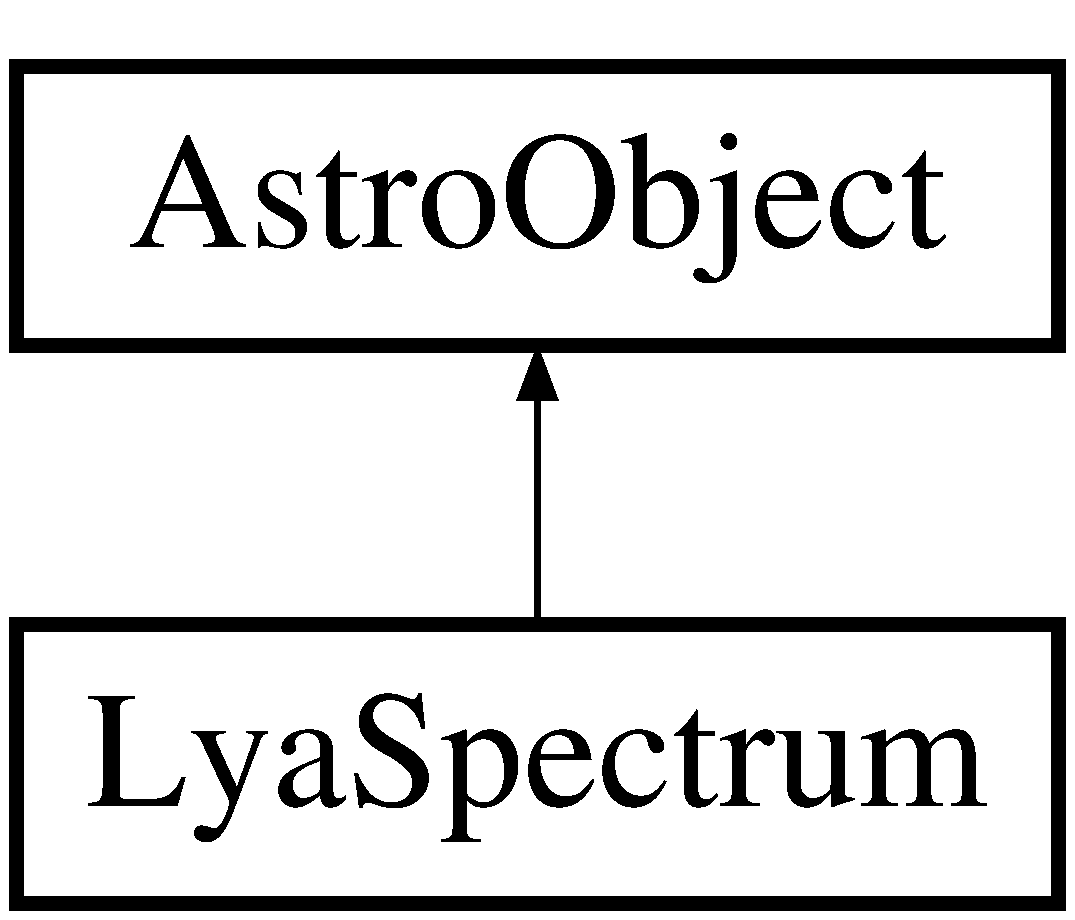
\includegraphics[height=2.000000cm]{class_astro_object}
\end{center}
\end{figure}
\subsection*{Public Member Functions}
\begin{DoxyCompactItemize}
\item 
\hyperlink{class_astro_object_a1802093595c886ac1e0f972829382c61}{Astro\-Object} ()
\item 
\hyperlink{class_astro_object_af5ff221d0cc120501f4e2c8b1c5ccfec}{Astro\-Object} (double \&ra, double \&dec, const int \&\hyperlink{class_astro_object_a2ebf8d94adab8f2f828a9209b1dc795e}{plate}, const int \&\hyperlink{class_astro_object_ab10c73e293654f21e73fcc344cf7d866}{fiber}, const int \&\hyperlink{class_astro_object_a4c54c4d7ad2f41eba2ff759c4fa3689b}{mjd}, const double \&\hyperlink{class_astro_object_a48a7db2aa513109f6cb662a44c36b3d3}{z}, const bool radians=true)
\item 
\hyperlink{class_sphere_point}{Sphere\-Point} \hyperlink{class_astro_object_a82d16c84459cdaab764205749660130b}{angle} () const 
\item 
double \hyperlink{class_astro_object_acb0a49a6cf2dc41076063a3b15b59b0f}{dist} () const 
\item 
int \hyperlink{class_astro_object_ab10c73e293654f21e73fcc344cf7d866}{fiber} () const 
\item 
int \hyperlink{class_astro_object_a4c54c4d7ad2f41eba2ff759c4fa3689b}{mjd} () const 
\item 
int \hyperlink{class_astro_object_a2ebf8d94adab8f2f828a9209b1dc795e}{plate} () const 
\item 
double \hyperlink{class_astro_object_a48a7db2aa513109f6cb662a44c36b3d3}{z} () const 
\item 
virtual void \hyperlink{class_astro_object_a7addd0f108191b1ca35db6e16e45ed72}{Set\-Distance} (const \hyperlink{class_interpolation_map}{Interpolation\-Map} \&redshift\-\_\-distance\-\_\-map)
\end{DoxyCompactItemize}
\subsection*{Protected Attributes}
\begin{DoxyCompactItemize}
\item 
\hyperlink{class_sphere_point}{Sphere\-Point} \hyperlink{class_astro_object_a78ea0158bd580946e621b534419bcd8f}{angle\-\_\-}
\item 
double \hyperlink{class_astro_object_a3644701bfa2f9de2343242e5fca7df86}{dist\-\_\-}
\item 
int \hyperlink{class_astro_object_a0f2dfed713d41bf6403b55ded214e044}{fiber\-\_\-}
\item 
int \hyperlink{class_astro_object_ac39bfb302dba24582e9f48147a30a320}{mjd\-\_\-}
\item 
int \hyperlink{class_astro_object_ac0b8a9a01565519345047fae0d6fe659}{plate\-\_\-}
\item 
double \hyperlink{class_astro_object_a07239818f3076c2a4ff0a3af0222b5e1}{z\-\_\-}
\end{DoxyCompactItemize}


\subsection{Detailed Description}
\hyperlink{astro__object_8h}{astro\-\_\-object.\-h} Purpose\-: This file defines the class \hyperlink{class_astro_object}{Astro\-Object}. This class contains the basic properties of any astronomical object and also some useful computation related with this properties

\begin{DoxyAuthor}{Author}
Ignasi Pérez-\/\-Ràfols (\href{mailto:iprafols@icc.ub.edu}{\tt iprafols@icc.\-ub.\-edu}) 
\end{DoxyAuthor}
\begin{DoxyVersion}{Version}
1.\-0 06/17/2014 
\end{DoxyVersion}


Definition at line 25 of file astro\-\_\-object.\-h.



\subsection{Constructor \& Destructor Documentation}
\hypertarget{class_astro_object_a1802093595c886ac1e0f972829382c61}{\index{Astro\-Object@{Astro\-Object}!Astro\-Object@{Astro\-Object}}
\index{Astro\-Object@{Astro\-Object}!AstroObject@{Astro\-Object}}
\subsubsection[{Astro\-Object}]{\setlength{\rightskip}{0pt plus 5cm}{\bf Astro\-Object\-::\-Astro\-Object} (
\begin{DoxyParamCaption}
{}
\end{DoxyParamCaption}
)\hspace{0.3cm}{\ttfamily  \mbox{[}inline\mbox{]}}}}\label{class_astro_object_a1802093595c886ac1e0f972829382c61}


Definition at line 32 of file astro\-\_\-object.\-h.


\begin{DoxyCode}
{};
\end{DoxyCode}
\hypertarget{class_astro_object_af5ff221d0cc120501f4e2c8b1c5ccfec}{\index{Astro\-Object@{Astro\-Object}!Astro\-Object@{Astro\-Object}}
\index{Astro\-Object@{Astro\-Object}!AstroObject@{Astro\-Object}}
\subsubsection[{Astro\-Object}]{\setlength{\rightskip}{0pt plus 5cm}{\bf Astro\-Object\-::\-Astro\-Object} (
\begin{DoxyParamCaption}
\item[{double \&}]{ra, }
\item[{double \&}]{dec, }
\item[{const int \&}]{plate, }
\item[{const int \&}]{fiber, }
\item[{const int \&}]{mjd, }
\item[{const double \&}]{z, }
\item[{const bool}]{radians = {\ttfamily true}}
\end{DoxyParamCaption}
)}}\label{class_astro_object_af5ff221d0cc120501f4e2c8b1c5ccfec}
\hyperlink{astro__object_8cpp}{astro\-\_\-object.\-cpp} Purpose\-: This files contains the body for the functions defined in \hyperlink{astro__object_8h}{astro\-\_\-object.\-h}

\begin{DoxyAuthor}{Author}
Ignasi Pérez-\/\-Ràfols 
\end{DoxyAuthor}
\begin{DoxyVersion}{Version}
1.\-0 06/17/2014 
\end{DoxyVersion}
E\-X\-P\-L\-A\-N\-A\-T\-I\-O\-N\-: Cosntructs a \hyperlink{class_astro_object}{Astro\-Object} instance

I\-N\-P\-U\-T\-S\-: ra -\/ astronomical object's right ascension (in radians) dec -\/ astronomical object's declination (in radians) plate -\/ astronomical object's plate fiber -\/ astronomical object's fiber mjd -\/ astronomical object's Modified Jullian Date z -\/ astronomical object's redshift radians -\/ a boolean that specifies if the angles are given in radias -\/ defaul = True

O\-U\-T\-P\-U\-T\-S\-: N\-O\-N\-E

C\-L\-A\-S\-S\-E\-S U\-S\-E\-D\-: \hyperlink{class_astro_object}{Astro\-Object} \hyperlink{class_sphere_point}{Sphere\-Point}

F\-U\-N\-C\-I\-T\-O\-N\-S U\-S\-E\-D\-: N\-O\-N\-E

Definition at line 11 of file astro\-\_\-object.\-cpp.


\begin{DoxyCode}
                                                                               
                                                               {
    if (not radians){
        ra *= acos(-1)/180.0;
        dec *= acos(-1)/180.0;
    }
    SpherePoint angle(ra, dec);
    angle_ = angle;
    plate_ = plate;
    fiber_ = fiber;
    mjd_ = mjd;
    z_ = z;
}
\end{DoxyCode}


\subsection{Member Function Documentation}
\hypertarget{class_astro_object_a82d16c84459cdaab764205749660130b}{\index{Astro\-Object@{Astro\-Object}!angle@{angle}}
\index{angle@{angle}!AstroObject@{Astro\-Object}}
\subsubsection[{angle}]{\setlength{\rightskip}{0pt plus 5cm}{\bf Sphere\-Point} {\bf Astro\-Object\-::angle} (
\begin{DoxyParamCaption}
{}
\end{DoxyParamCaption}
) const\hspace{0.3cm}{\ttfamily  \mbox{[}inline\mbox{]}}}}\label{class_astro_object_a82d16c84459cdaab764205749660130b}


Definition at line 41 of file astro\-\_\-object.\-h.


\begin{DoxyCode}
{return angle_;}
\end{DoxyCode}
\hypertarget{class_astro_object_acb0a49a6cf2dc41076063a3b15b59b0f}{\index{Astro\-Object@{Astro\-Object}!dist@{dist}}
\index{dist@{dist}!AstroObject@{Astro\-Object}}
\subsubsection[{dist}]{\setlength{\rightskip}{0pt plus 5cm}double {\bf Astro\-Object\-::dist} (
\begin{DoxyParamCaption}
{}
\end{DoxyParamCaption}
) const\hspace{0.3cm}{\ttfamily  \mbox{[}inline\mbox{]}}}}\label{class_astro_object_acb0a49a6cf2dc41076063a3b15b59b0f}


Definition at line 44 of file astro\-\_\-object.\-h.


\begin{DoxyCode}
{return dist_;}
\end{DoxyCode}
\hypertarget{class_astro_object_ab10c73e293654f21e73fcc344cf7d866}{\index{Astro\-Object@{Astro\-Object}!fiber@{fiber}}
\index{fiber@{fiber}!AstroObject@{Astro\-Object}}
\subsubsection[{fiber}]{\setlength{\rightskip}{0pt plus 5cm}int {\bf Astro\-Object\-::fiber} (
\begin{DoxyParamCaption}
{}
\end{DoxyParamCaption}
) const\hspace{0.3cm}{\ttfamily  \mbox{[}inline\mbox{]}}}}\label{class_astro_object_ab10c73e293654f21e73fcc344cf7d866}


Definition at line 47 of file astro\-\_\-object.\-h.


\begin{DoxyCode}
{return fiber_;}
\end{DoxyCode}
\hypertarget{class_astro_object_a4c54c4d7ad2f41eba2ff759c4fa3689b}{\index{Astro\-Object@{Astro\-Object}!mjd@{mjd}}
\index{mjd@{mjd}!AstroObject@{Astro\-Object}}
\subsubsection[{mjd}]{\setlength{\rightskip}{0pt plus 5cm}int {\bf Astro\-Object\-::mjd} (
\begin{DoxyParamCaption}
{}
\end{DoxyParamCaption}
) const\hspace{0.3cm}{\ttfamily  \mbox{[}inline\mbox{]}}}}\label{class_astro_object_a4c54c4d7ad2f41eba2ff759c4fa3689b}


Definition at line 50 of file astro\-\_\-object.\-h.


\begin{DoxyCode}
{return mjd_;}
\end{DoxyCode}
\hypertarget{class_astro_object_a2ebf8d94adab8f2f828a9209b1dc795e}{\index{Astro\-Object@{Astro\-Object}!plate@{plate}}
\index{plate@{plate}!AstroObject@{Astro\-Object}}
\subsubsection[{plate}]{\setlength{\rightskip}{0pt plus 5cm}int {\bf Astro\-Object\-::plate} (
\begin{DoxyParamCaption}
{}
\end{DoxyParamCaption}
) const\hspace{0.3cm}{\ttfamily  \mbox{[}inline\mbox{]}}}}\label{class_astro_object_a2ebf8d94adab8f2f828a9209b1dc795e}


Definition at line 53 of file astro\-\_\-object.\-h.


\begin{DoxyCode}
{return plate_;}
\end{DoxyCode}
\hypertarget{class_astro_object_a7addd0f108191b1ca35db6e16e45ed72}{\index{Astro\-Object@{Astro\-Object}!Set\-Distance@{Set\-Distance}}
\index{Set\-Distance@{Set\-Distance}!AstroObject@{Astro\-Object}}
\subsubsection[{Set\-Distance}]{\setlength{\rightskip}{0pt plus 5cm}void {\bf Astro\-Object\-::\-Set\-Distance} (
\begin{DoxyParamCaption}
\item[{const {\bf Interpolation\-Map} \&}]{redshift\-\_\-distance\-\_\-map}
\end{DoxyParamCaption}
)\hspace{0.3cm}{\ttfamily  \mbox{[}virtual\mbox{]}}}}\label{class_astro_object_a7addd0f108191b1ca35db6e16e45ed72}
E\-X\-P\-L\-A\-N\-A\-T\-I\-O\-N\-: Sets the distance to object

I\-N\-P\-U\-T\-S\-: redshif\-\_\-distance\-\_\-map -\/ a \hyperlink{class_interpolation_map}{Interpolation\-Map} instance with the redshift-\/distance relation

O\-U\-T\-P\-U\-T\-S\-: N\-O\-N\-E

C\-L\-A\-S\-S\-E\-S U\-S\-E\-D\-: \hyperlink{class_astro_object}{Astro\-Object}

F\-U\-N\-C\-I\-T\-O\-N\-S U\-S\-E\-D\-: N\-O\-N\-E

Reimplemented in \hyperlink{class_lya_spectrum_a5aed91d841c38e3c399e2b84b05fd2d3}{Lya\-Spectrum}.



Definition at line 48 of file astro\-\_\-object.\-cpp.


\begin{DoxyCode}
                                                                          {
    dist_ = redshift_distance_map.LinearInterpolation(z_);
    
}
\end{DoxyCode}
\hypertarget{class_astro_object_a48a7db2aa513109f6cb662a44c36b3d3}{\index{Astro\-Object@{Astro\-Object}!z@{z}}
\index{z@{z}!AstroObject@{Astro\-Object}}
\subsubsection[{z}]{\setlength{\rightskip}{0pt plus 5cm}double {\bf Astro\-Object\-::z} (
\begin{DoxyParamCaption}
{}
\end{DoxyParamCaption}
) const\hspace{0.3cm}{\ttfamily  \mbox{[}inline\mbox{]}}}}\label{class_astro_object_a48a7db2aa513109f6cb662a44c36b3d3}


Definition at line 56 of file astro\-\_\-object.\-h.


\begin{DoxyCode}
{return z_;}
\end{DoxyCode}


\subsection{Member Data Documentation}
\hypertarget{class_astro_object_a78ea0158bd580946e621b534419bcd8f}{\index{Astro\-Object@{Astro\-Object}!angle\-\_\-@{angle\-\_\-}}
\index{angle\-\_\-@{angle\-\_\-}!AstroObject@{Astro\-Object}}
\subsubsection[{angle\-\_\-}]{\setlength{\rightskip}{0pt plus 5cm}{\bf Sphere\-Point} {\bf Astro\-Object\-::angle\-\_\-}\hspace{0.3cm}{\ttfamily  \mbox{[}protected\mbox{]}}}}\label{class_astro_object_a78ea0158bd580946e621b534419bcd8f}


Definition at line 70 of file astro\-\_\-object.\-h.

\hypertarget{class_astro_object_a3644701bfa2f9de2343242e5fca7df86}{\index{Astro\-Object@{Astro\-Object}!dist\-\_\-@{dist\-\_\-}}
\index{dist\-\_\-@{dist\-\_\-}!AstroObject@{Astro\-Object}}
\subsubsection[{dist\-\_\-}]{\setlength{\rightskip}{0pt plus 5cm}double {\bf Astro\-Object\-::dist\-\_\-}\hspace{0.3cm}{\ttfamily  \mbox{[}protected\mbox{]}}}}\label{class_astro_object_a3644701bfa2f9de2343242e5fca7df86}


Definition at line 73 of file astro\-\_\-object.\-h.

\hypertarget{class_astro_object_a0f2dfed713d41bf6403b55ded214e044}{\index{Astro\-Object@{Astro\-Object}!fiber\-\_\-@{fiber\-\_\-}}
\index{fiber\-\_\-@{fiber\-\_\-}!AstroObject@{Astro\-Object}}
\subsubsection[{fiber\-\_\-}]{\setlength{\rightskip}{0pt plus 5cm}int {\bf Astro\-Object\-::fiber\-\_\-}\hspace{0.3cm}{\ttfamily  \mbox{[}protected\mbox{]}}}}\label{class_astro_object_a0f2dfed713d41bf6403b55ded214e044}


Definition at line 76 of file astro\-\_\-object.\-h.

\hypertarget{class_astro_object_ac39bfb302dba24582e9f48147a30a320}{\index{Astro\-Object@{Astro\-Object}!mjd\-\_\-@{mjd\-\_\-}}
\index{mjd\-\_\-@{mjd\-\_\-}!AstroObject@{Astro\-Object}}
\subsubsection[{mjd\-\_\-}]{\setlength{\rightskip}{0pt plus 5cm}int {\bf Astro\-Object\-::mjd\-\_\-}\hspace{0.3cm}{\ttfamily  \mbox{[}protected\mbox{]}}}}\label{class_astro_object_ac39bfb302dba24582e9f48147a30a320}


Definition at line 79 of file astro\-\_\-object.\-h.

\hypertarget{class_astro_object_ac0b8a9a01565519345047fae0d6fe659}{\index{Astro\-Object@{Astro\-Object}!plate\-\_\-@{plate\-\_\-}}
\index{plate\-\_\-@{plate\-\_\-}!AstroObject@{Astro\-Object}}
\subsubsection[{plate\-\_\-}]{\setlength{\rightskip}{0pt plus 5cm}int {\bf Astro\-Object\-::plate\-\_\-}\hspace{0.3cm}{\ttfamily  \mbox{[}protected\mbox{]}}}}\label{class_astro_object_ac0b8a9a01565519345047fae0d6fe659}


Definition at line 82 of file astro\-\_\-object.\-h.

\hypertarget{class_astro_object_a07239818f3076c2a4ff0a3af0222b5e1}{\index{Astro\-Object@{Astro\-Object}!z\-\_\-@{z\-\_\-}}
\index{z\-\_\-@{z\-\_\-}!AstroObject@{Astro\-Object}}
\subsubsection[{z\-\_\-}]{\setlength{\rightskip}{0pt plus 5cm}double {\bf Astro\-Object\-::z\-\_\-}\hspace{0.3cm}{\ttfamily  \mbox{[}protected\mbox{]}}}}\label{class_astro_object_a07239818f3076c2a4ff0a3af0222b5e1}


Definition at line 85 of file astro\-\_\-object.\-h.



The documentation for this class was generated from the following files\-:\begin{DoxyCompactItemize}
\item 
\hyperlink{astro__object_8h}{astro\-\_\-object.\-h}\item 
\hyperlink{astro__object_8cpp}{astro\-\_\-object.\-cpp}\end{DoxyCompactItemize}

\hypertarget{class_astro_object_dataset}{\section{Astro\-Object\-Dataset Class Reference}
\label{class_astro_object_dataset}\index{Astro\-Object\-Dataset@{Astro\-Object\-Dataset}}
}


{\ttfamily \#include $<$astro\-\_\-object\-\_\-dataset.\-h$>$}

Inheritance diagram for Astro\-Object\-Dataset\-:\begin{figure}[H]
\begin{center}
\leavevmode
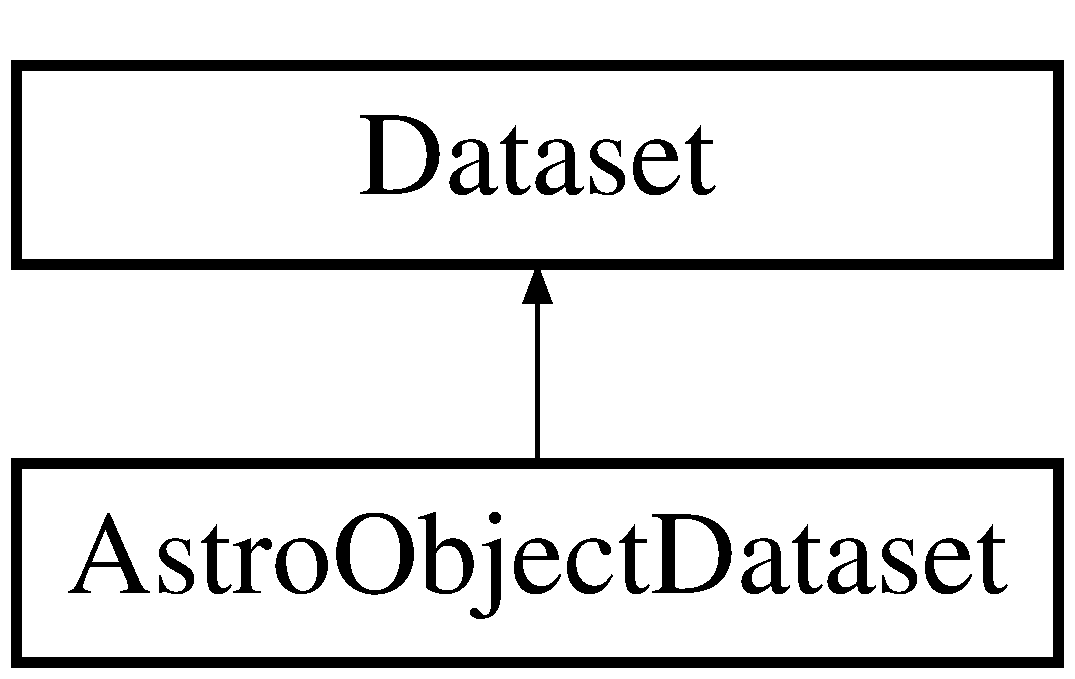
\includegraphics[height=2.000000cm]{class_astro_object_dataset}
\end{center}
\end{figure}
\subsection*{Public Member Functions}
\begin{DoxyCompactItemize}
\item 
\hyperlink{class_astro_object_dataset_aa75a72ea1b6dc3d9809cfac1b6c99f0a}{Astro\-Object\-Dataset} ()
\item 
\hyperlink{class_astro_object_dataset_a6962f42add89f7350a962324ac59ed89}{Astro\-Object\-Dataset} (const \hyperlink{class_global_variables}{Global\-Variables} \&k\-Global\-Variables)
\item 
\hyperlink{struct_plates_map_vector}{Plates\-Map\-Vector}$<$ \hyperlink{class_astro_object}{Astro\-Object} $>$\-::map \hyperlink{class_astro_object_dataset_a02751cdfdbd16f9d3a4d10a4f7e5173b}{list} () const 
\item 
std\-::vector$<$ \hyperlink{class_astro_object}{Astro\-Object} $>$ \hyperlink{class_astro_object_dataset_a87661176688f8709b08d5b950ed3d200}{list} (int plate\-\_\-number) const 
\item 
\hyperlink{class_astro_object}{Astro\-Object} \hyperlink{class_astro_object_dataset_a02d9f63962fefac8c89d29d9932c5e2b}{list} (int plate\-\_\-number, size\-\_\-t pos) const 
\item 
void \hyperlink{class_astro_object_dataset_a6dbee08285bbd1fba5b900e637ce5b2d}{Give\-R\-A\-D\-E\-C} (std\-::ostream \&out) const 
\item 
void \hyperlink{class_astro_object_dataset_a98c5a1ebf074c2589ed1e924bf5899bc}{Give\-Z} (std\-::ostream \&out) const 
\item 
void \hyperlink{class_astro_object_dataset_a7769e025efd79c249abcfc67bd653673}{Load} (const double \&z\-\_\-min, const double \&z\-\_\-max, const std\-::string \&object\-\_\-list)
\item 
void \hyperlink{class_astro_object_dataset_a4fe526d8aaf1f7e0182d5f30f82dcc60}{Set\-Distances} (const \hyperlink{class_interpolation_map}{Interpolation\-Map} \&redshift\-\_\-distance\-\_\-map)
\end{DoxyCompactItemize}


\subsection{Detailed Description}
\hyperlink{dataset_8h}{dataset.\-h} Purpose\-: This file defines the class \hyperlink{class_astro_object_dataset}{Astro\-Object\-Dataset}. This class contains the variables necessary to store a object dataset. This class is a specialization of the c\-Dataset class

\begin{DoxyAuthor}{Author}
Ignasi Pérez-\/\-Ràfols (\href{mailto:iprafols@icc.ub.edu}{\tt iprafols@icc.\-ub.\-edu}) 
\end{DoxyAuthor}
\begin{DoxyVersion}{Version}
1.\-0 07/25/2014 
\end{DoxyVersion}


Definition at line 37 of file astro\-\_\-object\-\_\-dataset.\-h.



\subsection{Constructor \& Destructor Documentation}
\hypertarget{class_astro_object_dataset_aa75a72ea1b6dc3d9809cfac1b6c99f0a}{\index{Astro\-Object\-Dataset@{Astro\-Object\-Dataset}!Astro\-Object\-Dataset@{Astro\-Object\-Dataset}}
\index{Astro\-Object\-Dataset@{Astro\-Object\-Dataset}!AstroObjectDataset@{Astro\-Object\-Dataset}}
\subsubsection[{Astro\-Object\-Dataset}]{\setlength{\rightskip}{0pt plus 5cm}{\bf Astro\-Object\-Dataset\-::\-Astro\-Object\-Dataset} (
\begin{DoxyParamCaption}
{}
\end{DoxyParamCaption}
)\hspace{0.3cm}{\ttfamily  \mbox{[}inline\mbox{]}}}}\label{class_astro_object_dataset_aa75a72ea1b6dc3d9809cfac1b6c99f0a}


Definition at line 44 of file astro\-\_\-object\-\_\-dataset.\-h.


\begin{DoxyCode}
{};
\end{DoxyCode}
\hypertarget{class_astro_object_dataset_a6962f42add89f7350a962324ac59ed89}{\index{Astro\-Object\-Dataset@{Astro\-Object\-Dataset}!Astro\-Object\-Dataset@{Astro\-Object\-Dataset}}
\index{Astro\-Object\-Dataset@{Astro\-Object\-Dataset}!AstroObjectDataset@{Astro\-Object\-Dataset}}
\subsubsection[{Astro\-Object\-Dataset}]{\setlength{\rightskip}{0pt plus 5cm}{\bf Astro\-Object\-Dataset\-::\-Astro\-Object\-Dataset} (
\begin{DoxyParamCaption}
\item[{const {\bf Global\-Variables} \&}]{k\-Global\-Variables}
\end{DoxyParamCaption}
)}}\label{class_astro_object_dataset_a6962f42add89f7350a962324ac59ed89}
\hyperlink{astro__object__dataset_8cpp}{astro\-\_\-object\-\_\-dataset.\-cpp} Purpose\-: This files contains the body for the functions defined in \hyperlink{astro__object__dataset_8h}{astro\-\_\-object\-\_\-dataset.\-h}

\begin{DoxyAuthor}{Author}
Ignasi Pérez-\/\-Ràfols 
\end{DoxyAuthor}
\begin{DoxyVersion}{Version}
1.\-0 08/08/2014 
\end{DoxyVersion}
E\-X\-P\-L\-A\-N\-A\-T\-I\-O\-N\-: Cosntructs a \hyperlink{class_astro_object_dataset}{Astro\-Object\-Dataset} instance and loads a catalog of Astro\-Objects into it

I\-N\-P\-U\-T\-S\-: k\-Global\-Varialbes -\/ object of type \hyperlink{class_global_variables}{Global\-Variables}

O\-U\-T\-P\-U\-T\-S\-: N\-O\-N\-E

C\-L\-A\-S\-S\-E\-S U\-S\-E\-D\-: \hyperlink{class_astro_object_dataset}{Astro\-Object\-Dataset} \hyperlink{class_global_variables}{Global\-Variables}

F\-U\-N\-C\-I\-T\-O\-N\-S U\-S\-E\-D\-: N\-O\-N\-E

Definition at line 13 of file astro\-\_\-object\-\_\-dataset.\-cpp.


\begin{DoxyCode}
                                                                             {
    name_ = kGlobalVariables.objects_catalog_name();
    Load(kGlobalVariables.z_min(), kGlobalVariables.z_max(), kGlobalVariables.
      objects_catalog());
    
}
\end{DoxyCode}


\subsection{Member Function Documentation}
\hypertarget{class_astro_object_dataset_a6dbee08285bbd1fba5b900e637ce5b2d}{\index{Astro\-Object\-Dataset@{Astro\-Object\-Dataset}!Give\-R\-A\-D\-E\-C@{Give\-R\-A\-D\-E\-C}}
\index{Give\-R\-A\-D\-E\-C@{Give\-R\-A\-D\-E\-C}!AstroObjectDataset@{Astro\-Object\-Dataset}}
\subsubsection[{Give\-R\-A\-D\-E\-C}]{\setlength{\rightskip}{0pt plus 5cm}void {\bf Astro\-Object\-Dataset\-::\-Give\-R\-A\-D\-E\-C} (
\begin{DoxyParamCaption}
\item[{std\-::ostream \&}]{out}
\end{DoxyParamCaption}
) const\hspace{0.3cm}{\ttfamily  \mbox{[}virtual\mbox{]}}}}\label{class_astro_object_dataset_a6dbee08285bbd1fba5b900e637ce5b2d}
E\-X\-P\-L\-A\-N\-A\-T\-I\-O\-N\-: Adds the objects' R\-A-\/\-D\-E\-C values to out

I\-N\-P\-U\-T\-S\-: out -\/ an ostream to add the objects' R\-A-\/\-D\-E\-C values to

O\-U\-T\-P\-U\-T\-S\-: N\-O\-N\-E

C\-L\-A\-S\-S\-E\-S U\-S\-E\-D\-: \hyperlink{class_astro_object}{Astro\-Object} \hyperlink{class_astro_object_dataset}{Astro\-Object\-Dataset}

F\-U\-N\-C\-I\-T\-O\-N\-S U\-S\-E\-D\-: N\-O\-N\-E

Implements \hyperlink{class_dataset_a5867a14c1554b50ce062bdacd36460af}{Dataset}.



Definition at line 37 of file astro\-\_\-object\-\_\-dataset.\-cpp.


\begin{DoxyCode}
                                                       {
    for (PlatesMapVector<AstroObject>::map::const_iterator it = list_.begin(); 
      it != list_.end(); it ++){
        for (size_t i = 0; i < (*it).second.size(); i ++){
            out << (*it).second[i].angle() << std::endl;
        }
    }
    
}
\end{DoxyCode}
\hypertarget{class_astro_object_dataset_a98c5a1ebf074c2589ed1e924bf5899bc}{\index{Astro\-Object\-Dataset@{Astro\-Object\-Dataset}!Give\-Z@{Give\-Z}}
\index{Give\-Z@{Give\-Z}!AstroObjectDataset@{Astro\-Object\-Dataset}}
\subsubsection[{Give\-Z}]{\setlength{\rightskip}{0pt plus 5cm}void {\bf Astro\-Object\-Dataset\-::\-Give\-Z} (
\begin{DoxyParamCaption}
\item[{std\-::ostream \&}]{out}
\end{DoxyParamCaption}
) const\hspace{0.3cm}{\ttfamily  \mbox{[}virtual\mbox{]}}}}\label{class_astro_object_dataset_a98c5a1ebf074c2589ed1e924bf5899bc}
E\-X\-P\-L\-A\-N\-A\-T\-I\-O\-N\-: Adds the objects' redshift values to out

I\-N\-P\-U\-T\-S\-: out -\/ an ostream to add the objects' redshift values to

O\-U\-T\-P\-U\-T\-S\-: N\-O\-N\-E

C\-L\-A\-S\-S\-E\-S U\-S\-E\-D\-: \hyperlink{class_astro_object}{Astro\-Object} \hyperlink{class_astro_object_dataset}{Astro\-Object\-Dataset}

F\-U\-N\-C\-I\-T\-O\-N\-S U\-S\-E\-D\-: N\-O\-N\-E

Implements \hyperlink{class_dataset_aae82d78ec374da243c22a96236b39465}{Dataset}.



Definition at line 64 of file astro\-\_\-object\-\_\-dataset.\-cpp.


\begin{DoxyCode}
                                                   {
    for (PlatesMapVector<AstroObject>::map::const_iterator it = list_.begin(); 
      it != list_.end(); it ++){
        for (size_t i = 0; i < (*it).second.size(); i ++){
            out << (*it).second[i].z() << std::endl;
        }
    }
    
}
\end{DoxyCode}
\hypertarget{class_astro_object_dataset_a02751cdfdbd16f9d3a4d10a4f7e5173b}{\index{Astro\-Object\-Dataset@{Astro\-Object\-Dataset}!list@{list}}
\index{list@{list}!AstroObjectDataset@{Astro\-Object\-Dataset}}
\subsubsection[{list}]{\setlength{\rightskip}{0pt plus 5cm}{\bf Plates\-Map\-Vector}$<${\bf Astro\-Object}$>$\-::map {\bf Astro\-Object\-Dataset\-::list} (
\begin{DoxyParamCaption}
{}
\end{DoxyParamCaption}
) const\hspace{0.3cm}{\ttfamily  \mbox{[}inline\mbox{]}}}}\label{class_astro_object_dataset_a02751cdfdbd16f9d3a4d10a4f7e5173b}


Definition at line 53 of file astro\-\_\-object\-\_\-dataset.\-h.


\begin{DoxyCode}
{return list_;}
\end{DoxyCode}
\hypertarget{class_astro_object_dataset_a87661176688f8709b08d5b950ed3d200}{\index{Astro\-Object\-Dataset@{Astro\-Object\-Dataset}!list@{list}}
\index{list@{list}!AstroObjectDataset@{Astro\-Object\-Dataset}}
\subsubsection[{list}]{\setlength{\rightskip}{0pt plus 5cm}std\-::vector$<${\bf Astro\-Object}$>$ {\bf Astro\-Object\-Dataset\-::list} (
\begin{DoxyParamCaption}
\item[{int}]{plate\-\_\-number}
\end{DoxyParamCaption}
) const\hspace{0.3cm}{\ttfamily  \mbox{[}inline\mbox{]}}}}\label{class_astro_object_dataset_a87661176688f8709b08d5b950ed3d200}


Definition at line 54 of file astro\-\_\-object\-\_\-dataset.\-h.


\begin{DoxyCode}
{return (*list_.find(plate_number)).second;}
\end{DoxyCode}
\hypertarget{class_astro_object_dataset_a02d9f63962fefac8c89d29d9932c5e2b}{\index{Astro\-Object\-Dataset@{Astro\-Object\-Dataset}!list@{list}}
\index{list@{list}!AstroObjectDataset@{Astro\-Object\-Dataset}}
\subsubsection[{list}]{\setlength{\rightskip}{0pt plus 5cm}{\bf Astro\-Object} {\bf Astro\-Object\-Dataset\-::list} (
\begin{DoxyParamCaption}
\item[{int}]{plate\-\_\-number, }
\item[{size\-\_\-t}]{pos}
\end{DoxyParamCaption}
) const\hspace{0.3cm}{\ttfamily  \mbox{[}inline\mbox{]}}}}\label{class_astro_object_dataset_a02d9f63962fefac8c89d29d9932c5e2b}


Definition at line 55 of file astro\-\_\-object\-\_\-dataset.\-h.


\begin{DoxyCode}
{return (*list_.find(plate_number)).second[pos];}
\end{DoxyCode}
\hypertarget{class_astro_object_dataset_a7769e025efd79c249abcfc67bd653673}{\index{Astro\-Object\-Dataset@{Astro\-Object\-Dataset}!Load@{Load}}
\index{Load@{Load}!AstroObjectDataset@{Astro\-Object\-Dataset}}
\subsubsection[{Load}]{\setlength{\rightskip}{0pt plus 5cm}void {\bf Astro\-Object\-Dataset\-::\-Load} (
\begin{DoxyParamCaption}
\item[{const double \&}]{z\-\_\-min, }
\item[{const double \&}]{z\-\_\-max, }
\item[{const std\-::string \&}]{object\-\_\-list}
\end{DoxyParamCaption}
)}}\label{class_astro_object_dataset_a7769e025efd79c249abcfc67bd653673}
E\-X\-P\-L\-A\-N\-A\-T\-I\-O\-N\-: Loads the object dataset from a catalog file

I\-N\-P\-U\-T\-S\-: z\-\_\-min -\/ minimum redshift to accept \hyperlink{class_astro_object}{Astro\-Object} into the dataset z\-\_\-max -\/ maximum redshift to accept \hyperlink{class_astro_object}{Astro\-Object} into the dataset objects\-\_\-catalog -\/ name of the catalog file

O\-U\-T\-P\-U\-T\-S\-: N\-O\-N\-E

C\-L\-A\-S\-S\-E\-S U\-S\-E\-D\-: \hyperlink{class_astro_object}{Astro\-Object} \hyperlink{class_astro_object_dataset}{Astro\-Object\-Dataset}

F\-U\-N\-C\-I\-T\-O\-N\-S U\-S\-E\-D\-: N\-O\-N\-E

Definition at line 91 of file astro\-\_\-object\-\_\-dataset.\-cpp.


\begin{DoxyCode}
                                                                               
                              {
    // setting the catalog columns to be read
    std::vector<std::string> fields(8);
    fields[0] = "PLATE";
    fields[1] = "MJD";
    fields[2] = "FIBERID";
    fields[3] = "RA";
    fields[4] = "DEC";
    fields[5] = "Z_VI";
    fields[6] = "PSFMAG";
    fields[7] = "SPECPRIMARY";
    
    // construct fits object
    std::auto_ptr<CCfits::FITS> pInfile; 
    
    try{
        
        pInfile = std::auto_ptr<CCfits::FITS>(new CCfits::FITS(objects_catalog,
      CCfits::Read,1,true,fields));
        
    } catch(CCfits::FITS::CantOpen x) {
        
        throw "Error occured in AstroObjectDataset constructor: couldn't open
       catalog file: " + objects_catalog;
    }
    CCfits::ExtHDU& data = pInfile->extension(1);
    
    // number of lines in the file
    long NAXIS2 = data.axis(1);
    size_t nobj = NAXIS2;
    
    // this will store the information
    std::valarray<int> plate,mjd,fiber;
    std::valarray<double> ra,dec,z;
    std::vector<valarray<double> > psf_mag;
    std::valarray<bool> boss_target1_flag,specprimary_flag;
    
    // reading data
    data.column(fields[0]).read(plate,1,nobj); // plate
    data.column(fields[1]).read(mjd,1,nobj); // mjd
    data.column(fields[2]).read(fiber,1,nobj); // fiber
    data.column(fields[3]).read(ra,1,nobj); // ra
    data.column(fields[4]).read(dec,1,nobj); // dec
    data.column(fields[5]).read(z,1,nobj); // z
    data.column(fields[6]).readArrays(psf_mag,1,nobj); // magnitudes
    data.column(fields[7]).read(specprimary_flag,1,nobj); // specprimary
    
    // setting size to zero and creating entries in list_ map
    size_ = 0;
    for (int i=0;i<nobj;i++){
        // this is to avoid repeated objects
        if (specprimary_flag[i] > 0){            
            
            if (list_.find(plate[i]) == list_.end()){
                std::vector<AstroObject> v;
                list_[plate[i]] = v;
                num_objects_in_plate_[plate[i]] = 0;
            }
            
        }
    }
    
    // adding objects to list_ and to list_by_plate
    for (int i=0;i<nobj;i++){
        // this is to avoid repeated objects
        if ((specprimary_flag[i] > 0) and (z_min <= z[i] and z[i] <= z_max) and
       not (ra[i] == 0.0 and dec[i] == 0.0)){
            
            // create AstroObject
            AstroObject object(ra[i], dec[i], plate[i], fiber[i], mjd[i], z[i],
       false);
            
            // adding object to list_
            (*list_.find(plate[i])).second.push_back(object);
            
            // updating size_
            size_ ++;
            
            // updating number_of_objects_in_plate
            (*num_objects_in_plate_.find(plate[i])).second ++;
            
        }
    }
    
}
\end{DoxyCode}
\hypertarget{class_astro_object_dataset_a4fe526d8aaf1f7e0182d5f30f82dcc60}{\index{Astro\-Object\-Dataset@{Astro\-Object\-Dataset}!Set\-Distances@{Set\-Distances}}
\index{Set\-Distances@{Set\-Distances}!AstroObjectDataset@{Astro\-Object\-Dataset}}
\subsubsection[{Set\-Distances}]{\setlength{\rightskip}{0pt plus 5cm}void {\bf Astro\-Object\-Dataset\-::\-Set\-Distances} (
\begin{DoxyParamCaption}
\item[{const {\bf Interpolation\-Map} \&}]{redshift\-\_\-distance\-\_\-map}
\end{DoxyParamCaption}
)\hspace{0.3cm}{\ttfamily  \mbox{[}virtual\mbox{]}}}}\label{class_astro_object_dataset_a4fe526d8aaf1f7e0182d5f30f82dcc60}
E\-X\-P\-L\-A\-N\-A\-T\-I\-O\-N\-: Sets the distance to every object in the dataset

I\-N\-P\-U\-T\-S\-: redshif\-\_\-distance\-\_\-map -\/ a \hyperlink{class_interpolation_map}{Interpolation\-Map} instance with the redshift-\/distance relation

O\-U\-T\-P\-U\-T\-S\-: N\-O\-N\-E

C\-L\-A\-S\-S\-E\-S U\-S\-E\-D\-: \hyperlink{class_astro_object}{Astro\-Object} \hyperlink{class_astro_object_dataset}{Astro\-Object\-Dataset} \hyperlink{class_interpolation_map}{Interpolation\-Map}

F\-U\-N\-C\-I\-T\-O\-N\-S U\-S\-E\-D\-: N\-O\-N\-E

Implements \hyperlink{class_dataset_a76dbae8574850da55a3b88149ccbe3f9}{Dataset}.



Definition at line 193 of file astro\-\_\-object\-\_\-dataset.\-cpp.


\begin{DoxyCode}
                                                                               
         {
    for (PlatesMapVector<AstroObject>::map::iterator it = list_.begin(); it != 
      list_.end(); it ++){
        for (size_t i = 0; i < (*it).second.size(); i ++){
            (*it).second[i].SetDistance(redshift_distance_map);
        }
    }
        
}
\end{DoxyCode}


The documentation for this class was generated from the following files\-:\begin{DoxyCompactItemize}
\item 
\hyperlink{astro__object__dataset_8h}{astro\-\_\-object\-\_\-dataset.\-h}\item 
\hyperlink{astro__object__dataset_8cpp}{astro\-\_\-object\-\_\-dataset.\-cpp}\end{DoxyCompactItemize}

\hypertarget{class_correlation_plate}{\section{Correlation\-Plate Class Reference}
\label{class_correlation_plate}\index{Correlation\-Plate@{Correlation\-Plate}}
}


{\ttfamily \#include $<$correlation\-\_\-plate.\-h$>$}

Inheritance diagram for Correlation\-Plate\-:\begin{figure}[H]
\begin{center}
\leavevmode
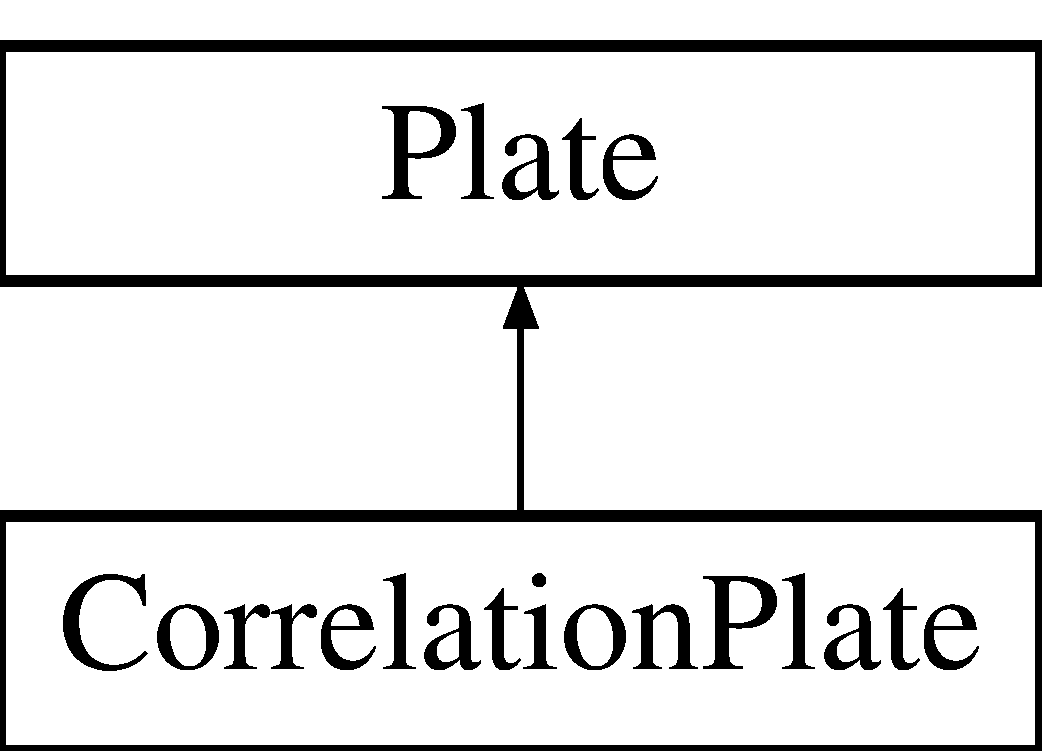
\includegraphics[height=2.000000cm]{class_correlation_plate}
\end{center}
\end{figure}
\subsection*{Public Member Functions}
\begin{DoxyCompactItemize}
\item 
\hyperlink{class_correlation_plate_a425183f37cd223a0cde0526e391b0558}{Correlation\-Plate} ()
\item 
\hyperlink{class_correlation_plate_a428b1a22cb7ed092b02546a89af1d8d1}{Correlation\-Plate} (const int \hyperlink{class_plate_a74d31939a29286c82ecd8fc7daf075ed}{plate\-\_\-number}, const size\-\_\-t \hyperlink{class_correlation_plate_a703ed8022866d1bbcc68bb5ae10ddbc3}{num\-\_\-bins}, const std\-::string \&\hyperlink{class_correlation_plate_a9af909d0d17ea8942c17b41e9379743c}{results}, const std\-::string \&\hyperlink{class_correlation_plate_a4b3fd30943868fb7c7e05bcad76d4e64}{pairs\-\_\-file\-\_\-name}, const std\-::vector$<$ int $>$ \&\hyperlink{class_correlation_plate_a197a4335cc4fbd6dab5b2da7431cbadc}{plate\-\_\-neighbours})
\item 
std\-::vector$<$ double $>$ \hyperlink{class_correlation_plate_a48f2550680d56a55bb7cf719a4ce65b2}{mean\-\_\-pi} () const 
\item 
double \hyperlink{class_correlation_plate_ab4c4d46291bfc8b7297e9fc2ac58512c}{mean\-\_\-pi} (size\-\_\-t index) const 
\item 
std\-::vector$<$ double $>$ \hyperlink{class_correlation_plate_aa1bbce0db890d496b7b60dd1e44d2894}{mean\-\_\-sigma} () const 
\item 
double \hyperlink{class_correlation_plate_a5344fb456d3b2a2172772c6d5b7dc777}{mean\-\_\-sigma} (size\-\_\-t index) const 
\item 
size\-\_\-t \hyperlink{class_correlation_plate_a703ed8022866d1bbcc68bb5ae10ddbc3}{num\-\_\-bins} () const 
\item 
std\-::vector$<$ int $>$ \hyperlink{class_correlation_plate_a9289ae56b96c65653388ab10074c29ee}{num\-\_\-averaged\-\_\-pairs} () const 
\item 
int \hyperlink{class_correlation_plate_ada9afe5f09d005fb9d0bf0f4787321fc}{num\-\_\-averaged\-\_\-pairs} (size\-\_\-t index) const 
\item 
std\-::string \hyperlink{class_correlation_plate_a4b3fd30943868fb7c7e05bcad76d4e64}{pairs\-\_\-file\-\_\-name} () const 
\item 
std\-::vector$<$ int $>$ \hyperlink{class_correlation_plate_a197a4335cc4fbd6dab5b2da7431cbadc}{plate\-\_\-neighbours} () const 
\item 
std\-::string \hyperlink{class_correlation_plate_a9af909d0d17ea8942c17b41e9379743c}{results} () const 
\item 
std\-::vector$<$ double $>$ \hyperlink{class_correlation_plate_a32f5eecab20e5e16c0782c8ba1769ea5}{weight} () const 
\item 
double \hyperlink{class_correlation_plate_a42507a70df5dd9f258ea626df83c578c}{weight} (size\-\_\-t index) const 
\item 
std\-::vector$<$ double $>$ \hyperlink{class_correlation_plate_ab3c49e88f49bb59fc6ee7f40c4b4fb66}{xi} () const 
\item 
double \hyperlink{class_correlation_plate_aa32ca0acce6b0562802f12400df1d13b}{xi} (size\-\_\-t index) const 
\item 
void \hyperlink{class_correlation_plate_a5a7760172439f8103abe425376d8415c}{Compute\-Cross\-Correlation} (const \hyperlink{class_astro_object_dataset}{Astro\-Object\-Dataset} \&object\-\_\-list, const \hyperlink{class_lya_spectra_dataset}{Lya\-Spectra\-Dataset} \&spectra\-\_\-list, const \hyperlink{class_global_variables}{Global\-Variables} \&k\-Global\-Variables)
\item 
std\-::string \hyperlink{class_correlation_plate_a3a6bfbe0c65cc4bb46ce4b4b43dc8d4e}{Info} (size\-\_\-t bin)
\item 
void \hyperlink{class_correlation_plate_a6e26de4b826cfd2b96d9d2d510f1e8e5}{Normalize} ()
\item 
void \hyperlink{class_correlation_plate_ac1d606757bd81c92e7c88387c59f5a1d}{operator+=} (const \hyperlink{class_correlation_plate}{Correlation\-Plate} \&other)
\end{DoxyCompactItemize}
\subsection*{Static Public Member Functions}
\begin{DoxyCompactItemize}
\item 
static std\-::string \hyperlink{class_correlation_plate_acefd722604a86e782cc773f80ef30bc9}{Info\-Header} ()
\end{DoxyCompactItemize}


\subsection{Detailed Description}
\hyperlink{correlation__plate_8h}{correlation\-\_\-plate.\-h} Purpose\-: This file defines the class \hyperlink{class_correlation_plate}{Correlation\-Plate}. This class contains the variables necessary to store the measurement of the cross-\/correlation in a single plate

\begin{DoxyAuthor}{Author}
Ignasi Pérez-\/\-Ràfols (\href{mailto:iprafols@icc.ub.edu}{\tt iprafols@icc.\-ub.\-edu}) 
\end{DoxyAuthor}
\begin{DoxyVersion}{Version}
1.\-0 10/02/2014 
\end{DoxyVersion}


Definition at line 37 of file correlation\-\_\-plate.\-h.



\subsection{Constructor \& Destructor Documentation}
\hypertarget{class_correlation_plate_a425183f37cd223a0cde0526e391b0558}{\index{Correlation\-Plate@{Correlation\-Plate}!Correlation\-Plate@{Correlation\-Plate}}
\index{Correlation\-Plate@{Correlation\-Plate}!CorrelationPlate@{Correlation\-Plate}}
\subsubsection[{Correlation\-Plate}]{\setlength{\rightskip}{0pt plus 5cm}{\bf Correlation\-Plate\-::\-Correlation\-Plate} (
\begin{DoxyParamCaption}
{}
\end{DoxyParamCaption}
)\hspace{0.3cm}{\ttfamily  \mbox{[}inline\mbox{]}}}}\label{class_correlation_plate_a425183f37cd223a0cde0526e391b0558}


Definition at line 44 of file correlation\-\_\-plate.\-h.


\begin{DoxyCode}
{};
\end{DoxyCode}
\hypertarget{class_correlation_plate_a428b1a22cb7ed092b02546a89af1d8d1}{\index{Correlation\-Plate@{Correlation\-Plate}!Correlation\-Plate@{Correlation\-Plate}}
\index{Correlation\-Plate@{Correlation\-Plate}!CorrelationPlate@{Correlation\-Plate}}
\subsubsection[{Correlation\-Plate}]{\setlength{\rightskip}{0pt plus 5cm}{\bf Correlation\-Plate\-::\-Correlation\-Plate} (
\begin{DoxyParamCaption}
\item[{const int}]{plate\-\_\-number, }
\item[{const size\-\_\-t}]{num\-\_\-bins, }
\item[{const std\-::string \&}]{results, }
\item[{const std\-::string \&}]{pairs\-\_\-file\-\_\-name, }
\item[{const std\-::vector$<$ int $>$ \&}]{plate\-\_\-neighbours}
\end{DoxyParamCaption}
)}}\label{class_correlation_plate_a428b1a22cb7ed092b02546a89af1d8d1}
\hyperlink{correlation__plate_8cpp}{correlation\-\_\-plate.\-cpp} Purpose\-: This files contains the body for the functions defined in \hyperlink{correlation__plate_8h}{correlation\-\_\-plate.\-h}

\begin{DoxyAuthor}{Author}
Ignasi Pérez-\/\-Ràfols 
\end{DoxyAuthor}
\begin{DoxyVersion}{Version}
1.\-0 10/02/2014 
\end{DoxyVersion}
E\-X\-P\-L\-A\-N\-A\-T\-I\-O\-N\-: Cosntructs a \hyperlink{class_correlation_plate}{Correlation\-Plate} instance and initializes all its variables

I\-N\-P\-U\-T\-S\-: plate\-\_\-number -\/ an integer with the plate number num\-\_\-bins -\/ an unsigned integer with the number of bins results -\/ a string with the path to the results directory (missing the bin number) pairs\-\_\-file\-\_\-name -\/ a string with the base name of the file storing the pairs information plate\-\_\-neighbours -\/ a vector containing the plate numbers of the neighbouring plates

O\-U\-T\-P\-U\-T\-S\-: N\-O\-N\-E

C\-L\-A\-S\-S\-E\-S U\-S\-E\-D\-: \hyperlink{class_correlation_plate}{Correlation\-Plate}

F\-U\-N\-C\-I\-T\-O\-N\-S U\-S\-E\-D\-: To\-Str

Definition at line 11 of file correlation\-\_\-plate.\-cpp.


\begin{DoxyCode}
                                                                               
                                                                                      
                          {
    plate_number_ = plate_number;
    plate_neighbours_ = plate_neighbours;
    num_bins_ = num_bins;
    if (plate_number_ == _NORM_){
        results_ = "";
        pairs_file_name_ = pairs_file_name;
    }
    else{
        results_ = results;
        pairs_file_name_ = "/" + pairs_file_name + ToStr(plate_number_) + ".dat
      ";
    }
    
    xi_.resize(num_bins_,0.0);
    mean_pi_.resize(num_bins_,0.0);
    mean_sigma_.resize(num_bins_,0.0);
    weight_.resize(num_bins_,0.0);
    num_averaged_pairs_.resize(num_bins_,0);

}
\end{DoxyCode}


\subsection{Member Function Documentation}
\hypertarget{class_correlation_plate_a5a7760172439f8103abe425376d8415c}{\index{Correlation\-Plate@{Correlation\-Plate}!Compute\-Cross\-Correlation@{Compute\-Cross\-Correlation}}
\index{Compute\-Cross\-Correlation@{Compute\-Cross\-Correlation}!CorrelationPlate@{Correlation\-Plate}}
\subsubsection[{Compute\-Cross\-Correlation}]{\setlength{\rightskip}{0pt plus 5cm}void {\bf Correlation\-Plate\-::\-Compute\-Cross\-Correlation} (
\begin{DoxyParamCaption}
\item[{const {\bf Astro\-Object\-Dataset} \&}]{object\-\_\-list, }
\item[{const {\bf Lya\-Spectra\-Dataset} \&}]{spectra\-\_\-list, }
\item[{const {\bf Global\-Variables} \&}]{k\-Global\-Variables}
\end{DoxyParamCaption}
)}}\label{class_correlation_plate_a5a7760172439f8103abe425376d8415c}
E\-X\-P\-L\-A\-N\-A\-T\-I\-O\-N\-: Computes the cross-\/correlation

I\-N\-P\-U\-T\-S\-: object\-\_\-list -\/ an \hyperlink{class_astro_object_dataset}{Astro\-Object\-Dataset} instance spectra\-\_\-list -\/ a \hyperlink{class_lya_spectra_dataset}{Lya\-Spectra\-Dataset} instance k\-Global\-Variables -\/ a \hyperlink{class_global_variables}{Global\-Variables} instance to load bin settings

O\-U\-T\-P\-U\-T\-S\-: N\-O\-N\-E

C\-L\-A\-S\-S\-E\-S U\-S\-E\-D\-: \hyperlink{class_astro_object_dataset}{Astro\-Object\-Dataset} \hyperlink{class_correlation_plate}{Correlation\-Plate} G\-Lobal\-Variables \hyperlink{class_lya_pixel}{Lya\-Pixel} \hyperlink{class_lya_spectra_dataset}{Lya\-Spectra\-Dataset} \hyperlink{class_lya_spectrum}{Lya\-Spectrum}

F\-U\-N\-C\-I\-T\-O\-N\-S U\-S\-E\-D\-: N\-O\-N\-E

Definition at line 83 of file correlation\-\_\-plate.\-cpp.


\begin{DoxyCode}
                                                                               
                                                                                      
          {
    // load bin settings
    double max_pi = kGlobalVariables.max_pi();
    double max_sigma = kGlobalVariables.max_sigma();
    double step_pi = kGlobalVariables.step_pi();
    double step_sigma = kGlobalVariables.step_sigma();
    double num_pi_bins = kGlobalVariables.num_pi_bins();
    double num_sigma_bins = kGlobalVariables.num_sigma_bins();    
    
    size_t number_of_objects = object_list.num_objects_in_plate(plate_number_);
    
    //std::cout << "computing cross-correlation in plate " << plate_number_ <<
       "; in this plate there are " << number_of_objects << " AstroObjects" <<
       std::endl;

    // loop over AstroObjects
    for (size_t i = 0; i < number_of_objects; i ++){
        AstroObject object = object_list.list(plate_number_, i);
                
        double sigma_aux_o = 2.0*object.dist(); // auxiliar variable to compute
       sigma values
        
        // loop over neighbouring plates
        for (size_t j = 0; j < plate_neighbours_.size(); j ++){
            
            size_t number_of_spectra = spectra_list.num_objects_in_plate(
      plate_neighbours_[j]);
            
            // loop over LyaSpectra
            for (size_t k = 0; k < number_of_spectra; k ++){

                LyaSpectrum lya_spectrum = spectra_list.list(plate_neighbours_[
      j], k);
                std::vector<LyaPixel> spectrum = lya_spectrum.spectrum();
                
                // compute angular separation
                double cos_theta = object.angle().CosAngularDistance(
      lya_spectrum.angle());
                
                double sigma_aux = sigma_aux_o*(1.0-cos_theta); // auxiliar
       variable to compute sigma values
                
                // check if all pixels in the spectrum are too far apart
                double pair_min_sigma = sqrt(sigma_aux*spectrum[0].dist()); //
       minimum distance obtained for lowest redshift pixel
                if (pair_min_sigma > max_sigma){ // if the minimum value for
       sigma (r_perp) is too large, the whole spectra is discarded
                    //std::cout << "TEST: spectra rejected because min_sigma is
       too large. value = " << pair_min_sigma << std::endl;
                    //std::cout << "TEST: ra_object dec_object ra_spectra
       dec_spectra cos_theta theta min_sigma" << std::endl;
                    //std::cout << "TEST: " << object.angle() << " " <<
       lya_spectrum.angle() << " " << cos_theta << " " << acos(cos_theta) << " " <<
       pair_min_sigma << std::endl;
                    continue;
                } 
                
                double pair_max_pi = object.dist()-spectrum[0].dist(); //
       minimum distance obtained for lowest redshift pixel
                if (pair_max_pi < -max_pi) { // if maximum value for pi (r_par)
       is too small, the whole spectra is discarded
                    //std::cout << "TEST: spectra rejected because min_pi is
       too small" << std::endl;
                    continue;
                }
                double pair_min_pi = object.dist()-spectrum.back().dist(); //
       maximum distance obtained for highest redshift pixel
                if (pair_min_pi>max_pi){ // if minimum value for pi (r_par) is
       too high, the whole spectrum is discarded
                    //std::cout << "TEST: spectra rejected because min_pi is
       too large" << std::endl;
                    continue;
                }
                
                // loop over LyaPixels
                for (int p = 0; p < spectrum.size(); p ++){
                    
                    // compute pi and sigma
                    double sigma = sqrt(sigma_aux*spectrum[p].dist());
                    if (sigma > max_sigma){ // if sigma (r_perp) is too large,
       discard pixel
                        continue;
                    }
                    double pi = object.dist()-spectrum[p].dist();
                    if ((pi > max_pi) or (pi <- max_pi)){ // if pi (r_par) is
       too large or too small, discard pixel
                        continue;
                    }
                    
                    //std::cout << "TEST: accepted pixel" << std::endl;
                    // locate pi pixel (i_index)
                    int i_index = int(pi/step_pi)+num_pi_bins/2;
                    if (pi<0.0){
                        i_index -= 1;
                    }
                    
                    // locate sigma pixel (j_index)
                    int j_index = int(sigma/step_sigma);
                    
                    // locate xi pixel (k)
                    int k_index = i_index*num_sigma_bins+j_index;
                    
                    // add contribution to xi in the specified bin
                    AddPair(k_index, spectrum[p], pi, sigma);
                    
                    // write down pair information in bin file
                    SavePair(k_index, object, lya_spectrum, p, pi, sigma);
                }
            }
        }
    }
}
\end{DoxyCode}
\hypertarget{class_correlation_plate_a3a6bfbe0c65cc4bb46ce4b4b43dc8d4e}{\index{Correlation\-Plate@{Correlation\-Plate}!Info@{Info}}
\index{Info@{Info}!CorrelationPlate@{Correlation\-Plate}}
\subsubsection[{Info}]{\setlength{\rightskip}{0pt plus 5cm}std\-::string {\bf Correlation\-Plate\-::\-Info} (
\begin{DoxyParamCaption}
\item[{size\-\_\-t}]{bin}
\end{DoxyParamCaption}
)}}\label{class_correlation_plate_a3a6bfbe0c65cc4bb46ce4b4b43dc8d4e}
E\-X\-P\-L\-A\-N\-A\-T\-I\-O\-N\-: Returns a string with the information for the selected bin

I\-N\-P\-U\-T\-S\-: bin -\/ an unsigned integral specifying the bin

O\-U\-T\-P\-U\-T\-S\-: out -\/ a string with the information

C\-L\-A\-S\-S\-E\-S U\-S\-E\-D\-: \hyperlink{class_correlation_plate}{Correlation\-Plate}

F\-U\-N\-C\-I\-T\-O\-N\-S U\-S\-E\-D\-: To\-Str

Definition at line 199 of file correlation\-\_\-plate.\-cpp.


\begin{DoxyCode}
                                          {
    string out = "";
    
    out += ToStr(plate_number_) + " " + ToStr(xi_[bin]) + " " + ToStr(mean_pi_[
      bin]) + " " + ToStr(mean_sigma_[bin]) + " " + ToStr(weight_[bin]) + " " + ToStr(
      num_averaged_pairs_[bin]);
    
    return out;
}
\end{DoxyCode}
\hypertarget{class_correlation_plate_acefd722604a86e782cc773f80ef30bc9}{\index{Correlation\-Plate@{Correlation\-Plate}!Info\-Header@{Info\-Header}}
\index{Info\-Header@{Info\-Header}!CorrelationPlate@{Correlation\-Plate}}
\subsubsection[{Info\-Header}]{\setlength{\rightskip}{0pt plus 5cm}std\-::string {\bf Correlation\-Plate\-::\-Info\-Header} (
\begin{DoxyParamCaption}
{}
\end{DoxyParamCaption}
)\hspace{0.3cm}{\ttfamily  \mbox{[}static\mbox{]}}}}\label{class_correlation_plate_acefd722604a86e782cc773f80ef30bc9}
E\-X\-P\-L\-A\-N\-A\-T\-I\-O\-N\-: Returns a string with the columns information

I\-N\-P\-U\-T\-S\-: N\-O\-N\-E

O\-U\-T\-P\-U\-T\-S\-: a string with the information

C\-L\-A\-S\-S\-E\-S U\-S\-E\-D\-: N\-O\-N\-E

F\-U\-N\-C\-I\-T\-O\-N\-S U\-S\-E\-D\-: N\-O\-N\-E

Definition at line 223 of file correlation\-\_\-plate.\-cpp.


\begin{DoxyCode}
                                      {
    return "# plate xi mean_pi mean_sigma weight num_averaged_pairs";
}
\end{DoxyCode}
\hypertarget{class_correlation_plate_a48f2550680d56a55bb7cf719a4ce65b2}{\index{Correlation\-Plate@{Correlation\-Plate}!mean\-\_\-pi@{mean\-\_\-pi}}
\index{mean\-\_\-pi@{mean\-\_\-pi}!CorrelationPlate@{Correlation\-Plate}}
\subsubsection[{mean\-\_\-pi}]{\setlength{\rightskip}{0pt plus 5cm}std\-::vector$<$double$>$ {\bf Correlation\-Plate\-::mean\-\_\-pi} (
\begin{DoxyParamCaption}
{}
\end{DoxyParamCaption}
) const\hspace{0.3cm}{\ttfamily  \mbox{[}inline\mbox{]}}}}\label{class_correlation_plate_a48f2550680d56a55bb7cf719a4ce65b2}


Definition at line 53 of file correlation\-\_\-plate.\-h.


\begin{DoxyCode}
{return mean_pi_;}
\end{DoxyCode}
\hypertarget{class_correlation_plate_ab4c4d46291bfc8b7297e9fc2ac58512c}{\index{Correlation\-Plate@{Correlation\-Plate}!mean\-\_\-pi@{mean\-\_\-pi}}
\index{mean\-\_\-pi@{mean\-\_\-pi}!CorrelationPlate@{Correlation\-Plate}}
\subsubsection[{mean\-\_\-pi}]{\setlength{\rightskip}{0pt plus 5cm}double {\bf Correlation\-Plate\-::mean\-\_\-pi} (
\begin{DoxyParamCaption}
\item[{size\-\_\-t}]{index}
\end{DoxyParamCaption}
) const\hspace{0.3cm}{\ttfamily  \mbox{[}inline\mbox{]}}}}\label{class_correlation_plate_ab4c4d46291bfc8b7297e9fc2ac58512c}


Definition at line 54 of file correlation\-\_\-plate.\-h.


\begin{DoxyCode}
{return mean_pi_[index];}
\end{DoxyCode}
\hypertarget{class_correlation_plate_aa1bbce0db890d496b7b60dd1e44d2894}{\index{Correlation\-Plate@{Correlation\-Plate}!mean\-\_\-sigma@{mean\-\_\-sigma}}
\index{mean\-\_\-sigma@{mean\-\_\-sigma}!CorrelationPlate@{Correlation\-Plate}}
\subsubsection[{mean\-\_\-sigma}]{\setlength{\rightskip}{0pt plus 5cm}std\-::vector$<$double$>$ {\bf Correlation\-Plate\-::mean\-\_\-sigma} (
\begin{DoxyParamCaption}
{}
\end{DoxyParamCaption}
) const\hspace{0.3cm}{\ttfamily  \mbox{[}inline\mbox{]}}}}\label{class_correlation_plate_aa1bbce0db890d496b7b60dd1e44d2894}


Definition at line 57 of file correlation\-\_\-plate.\-h.


\begin{DoxyCode}
{return mean_sigma_;}
\end{DoxyCode}
\hypertarget{class_correlation_plate_a5344fb456d3b2a2172772c6d5b7dc777}{\index{Correlation\-Plate@{Correlation\-Plate}!mean\-\_\-sigma@{mean\-\_\-sigma}}
\index{mean\-\_\-sigma@{mean\-\_\-sigma}!CorrelationPlate@{Correlation\-Plate}}
\subsubsection[{mean\-\_\-sigma}]{\setlength{\rightskip}{0pt plus 5cm}double {\bf Correlation\-Plate\-::mean\-\_\-sigma} (
\begin{DoxyParamCaption}
\item[{size\-\_\-t}]{index}
\end{DoxyParamCaption}
) const\hspace{0.3cm}{\ttfamily  \mbox{[}inline\mbox{]}}}}\label{class_correlation_plate_a5344fb456d3b2a2172772c6d5b7dc777}


Definition at line 58 of file correlation\-\_\-plate.\-h.


\begin{DoxyCode}
{return mean_sigma_[index];}
\end{DoxyCode}
\hypertarget{class_correlation_plate_a6e26de4b826cfd2b96d9d2d510f1e8e5}{\index{Correlation\-Plate@{Correlation\-Plate}!Normalize@{Normalize}}
\index{Normalize@{Normalize}!CorrelationPlate@{Correlation\-Plate}}
\subsubsection[{Normalize}]{\setlength{\rightskip}{0pt plus 5cm}void {\bf Correlation\-Plate\-::\-Normalize} (
\begin{DoxyParamCaption}
{}
\end{DoxyParamCaption}
)}}\label{class_correlation_plate_a6e26de4b826cfd2b96d9d2d510f1e8e5}
E\-X\-P\-L\-A\-N\-A\-T\-I\-O\-N\-: Normalizes the cross correlation results

I\-N\-P\-U\-T\-S\-: N\-O\-N\-E

O\-U\-T\-P\-U\-T\-S\-: N\-O\-N\-E

C\-L\-A\-S\-S\-E\-S U\-S\-E\-D\-: \hyperlink{class_correlation_plate}{Correlation\-Plate}

F\-U\-N\-C\-I\-T\-O\-N\-S U\-S\-E\-D\-: N\-O\-N\-E

Reimplemented from \hyperlink{class_plate_af8c7b2cbadfd5359e7464f6015cbf21c}{Plate}.



Definition at line 244 of file correlation\-\_\-plate.\-cpp.


\begin{DoxyCode}
                                {
    if (plate_number_ == _NORM_){
        
        for (size_t i = 0; i < num_bins_; i ++){
            
            if (weight_[i] == 0.0){
                // if the weight is zero, complain and exit the function
                std::cout << "Zero Division Error in Correlation::Normalize,
       aborting..." << std::endl;
                return;
            }
            // if the weight is 1.0, normalization is not needed
            else if (weight_[i] != 1.0){
                
                xi_[i] /= weight_[i];
                mean_pi_[i] /= weight_[i];
                mean_sigma_[i] /= weight_[i];
                weight_[i] = 1.0;
            }
            
        }
        
    }
    else{
        // if plate number is not _NORM_, the instance is not supposed to
       normalize
        std::cout << "Warning: Plate number is not set to _NORM_. This
       CorrelationPlate instance should not be normalized. Ignoring..." << std::endl;
    }
    
}
\end{DoxyCode}
\hypertarget{class_correlation_plate_a9289ae56b96c65653388ab10074c29ee}{\index{Correlation\-Plate@{Correlation\-Plate}!num\-\_\-averaged\-\_\-pairs@{num\-\_\-averaged\-\_\-pairs}}
\index{num\-\_\-averaged\-\_\-pairs@{num\-\_\-averaged\-\_\-pairs}!CorrelationPlate@{Correlation\-Plate}}
\subsubsection[{num\-\_\-averaged\-\_\-pairs}]{\setlength{\rightskip}{0pt plus 5cm}std\-::vector$<$int$>$ {\bf Correlation\-Plate\-::num\-\_\-averaged\-\_\-pairs} (
\begin{DoxyParamCaption}
{}
\end{DoxyParamCaption}
) const\hspace{0.3cm}{\ttfamily  \mbox{[}inline\mbox{]}}}}\label{class_correlation_plate_a9289ae56b96c65653388ab10074c29ee}


Definition at line 64 of file correlation\-\_\-plate.\-h.


\begin{DoxyCode}
{return num_averaged_pairs_;}
\end{DoxyCode}
\hypertarget{class_correlation_plate_ada9afe5f09d005fb9d0bf0f4787321fc}{\index{Correlation\-Plate@{Correlation\-Plate}!num\-\_\-averaged\-\_\-pairs@{num\-\_\-averaged\-\_\-pairs}}
\index{num\-\_\-averaged\-\_\-pairs@{num\-\_\-averaged\-\_\-pairs}!CorrelationPlate@{Correlation\-Plate}}
\subsubsection[{num\-\_\-averaged\-\_\-pairs}]{\setlength{\rightskip}{0pt plus 5cm}int {\bf Correlation\-Plate\-::num\-\_\-averaged\-\_\-pairs} (
\begin{DoxyParamCaption}
\item[{size\-\_\-t}]{index}
\end{DoxyParamCaption}
) const\hspace{0.3cm}{\ttfamily  \mbox{[}inline\mbox{]}}}}\label{class_correlation_plate_ada9afe5f09d005fb9d0bf0f4787321fc}


Definition at line 65 of file correlation\-\_\-plate.\-h.


\begin{DoxyCode}
{return num_averaged_pairs_[index];}
\end{DoxyCode}
\hypertarget{class_correlation_plate_a703ed8022866d1bbcc68bb5ae10ddbc3}{\index{Correlation\-Plate@{Correlation\-Plate}!num\-\_\-bins@{num\-\_\-bins}}
\index{num\-\_\-bins@{num\-\_\-bins}!CorrelationPlate@{Correlation\-Plate}}
\subsubsection[{num\-\_\-bins}]{\setlength{\rightskip}{0pt plus 5cm}size\-\_\-t {\bf Correlation\-Plate\-::num\-\_\-bins} (
\begin{DoxyParamCaption}
{}
\end{DoxyParamCaption}
) const\hspace{0.3cm}{\ttfamily  \mbox{[}inline\mbox{]}}}}\label{class_correlation_plate_a703ed8022866d1bbcc68bb5ae10ddbc3}


Definition at line 61 of file correlation\-\_\-plate.\-h.


\begin{DoxyCode}
{return num_bins_;}
\end{DoxyCode}
\hypertarget{class_correlation_plate_ac1d606757bd81c92e7c88387c59f5a1d}{\index{Correlation\-Plate@{Correlation\-Plate}!operator+=@{operator+=}}
\index{operator+=@{operator+=}!CorrelationPlate@{Correlation\-Plate}}
\subsubsection[{operator+=}]{\setlength{\rightskip}{0pt plus 5cm}void Correlation\-Plate\-::operator+= (
\begin{DoxyParamCaption}
\item[{const {\bf Correlation\-Plate} \&}]{other}
\end{DoxyParamCaption}
)}}\label{class_correlation_plate_ac1d606757bd81c92e7c88387c59f5a1d}
E\-X\-P\-L\-A\-N\-A\-T\-I\-O\-N\-: Overloads the += operator. Updates the xi\-\_\-, mean\-\_\-sigma, mean\-\_\-pi and weight\-\_\- values by adding those in other.

I\-N\-P\-U\-T\-S\-: other -\/ a \hyperlink{class_correlation_plate}{Correlation\-Plate} instance to be added

O\-U\-T\-P\-U\-T\-S\-: N\-O\-N\-E

C\-L\-A\-S\-S\-E\-S U\-S\-E\-D\-: \hyperlink{class_correlation_plate}{Correlation\-Plate}

F\-U\-N\-C\-I\-T\-O\-N\-S U\-S\-E\-D\-: N\-O\-N\-E

Definition at line 333 of file correlation\-\_\-plate.\-cpp.


\begin{DoxyCode}
                                                               {
    // check that both instances have the same number of bins
    if (num_bins_ == other.num_bins()){
        for (size_t i = 0; i < num_bins_; i ++){
            xi_[i] += other.xi(i);
            mean_pi_[i] += other.mean_pi(i);
            mean_sigma_[i] += other.mean_sigma(i);
            weight_[i] += other.weight(i);
            num_averaged_pairs_[i] += other.num_averaged_pairs(i);
        }
        
    }
    // if they don't, complain
    else{
        std::cout << "Warning: Trying to add CorrelationPlates with different
       number of bins. Ignoring..." << std::endl;
    }
    
    
}
\end{DoxyCode}
\hypertarget{class_correlation_plate_a4b3fd30943868fb7c7e05bcad76d4e64}{\index{Correlation\-Plate@{Correlation\-Plate}!pairs\-\_\-file\-\_\-name@{pairs\-\_\-file\-\_\-name}}
\index{pairs\-\_\-file\-\_\-name@{pairs\-\_\-file\-\_\-name}!CorrelationPlate@{Correlation\-Plate}}
\subsubsection[{pairs\-\_\-file\-\_\-name}]{\setlength{\rightskip}{0pt plus 5cm}std\-::string {\bf Correlation\-Plate\-::pairs\-\_\-file\-\_\-name} (
\begin{DoxyParamCaption}
{}
\end{DoxyParamCaption}
) const\hspace{0.3cm}{\ttfamily  \mbox{[}inline\mbox{]}}}}\label{class_correlation_plate_a4b3fd30943868fb7c7e05bcad76d4e64}


Definition at line 68 of file correlation\-\_\-plate.\-h.


\begin{DoxyCode}
{return pairs_file_name_;}
\end{DoxyCode}
\hypertarget{class_correlation_plate_a197a4335cc4fbd6dab5b2da7431cbadc}{\index{Correlation\-Plate@{Correlation\-Plate}!plate\-\_\-neighbours@{plate\-\_\-neighbours}}
\index{plate\-\_\-neighbours@{plate\-\_\-neighbours}!CorrelationPlate@{Correlation\-Plate}}
\subsubsection[{plate\-\_\-neighbours}]{\setlength{\rightskip}{0pt plus 5cm}std\-::vector$<$int$>$ {\bf Correlation\-Plate\-::plate\-\_\-neighbours} (
\begin{DoxyParamCaption}
{}
\end{DoxyParamCaption}
) const\hspace{0.3cm}{\ttfamily  \mbox{[}inline\mbox{]}}}}\label{class_correlation_plate_a197a4335cc4fbd6dab5b2da7431cbadc}


Definition at line 71 of file correlation\-\_\-plate.\-h.


\begin{DoxyCode}
{return plate_neighbours_;}
\end{DoxyCode}
\hypertarget{class_correlation_plate_a9af909d0d17ea8942c17b41e9379743c}{\index{Correlation\-Plate@{Correlation\-Plate}!results@{results}}
\index{results@{results}!CorrelationPlate@{Correlation\-Plate}}
\subsubsection[{results}]{\setlength{\rightskip}{0pt plus 5cm}std\-::string {\bf Correlation\-Plate\-::results} (
\begin{DoxyParamCaption}
{}
\end{DoxyParamCaption}
) const\hspace{0.3cm}{\ttfamily  \mbox{[}inline\mbox{]}}}}\label{class_correlation_plate_a9af909d0d17ea8942c17b41e9379743c}


Definition at line 74 of file correlation\-\_\-plate.\-h.


\begin{DoxyCode}
{return results_;}
\end{DoxyCode}
\hypertarget{class_correlation_plate_a32f5eecab20e5e16c0782c8ba1769ea5}{\index{Correlation\-Plate@{Correlation\-Plate}!weight@{weight}}
\index{weight@{weight}!CorrelationPlate@{Correlation\-Plate}}
\subsubsection[{weight}]{\setlength{\rightskip}{0pt plus 5cm}std\-::vector$<$double$>$ {\bf Correlation\-Plate\-::weight} (
\begin{DoxyParamCaption}
{}
\end{DoxyParamCaption}
) const\hspace{0.3cm}{\ttfamily  \mbox{[}inline\mbox{]}}}}\label{class_correlation_plate_a32f5eecab20e5e16c0782c8ba1769ea5}


Definition at line 77 of file correlation\-\_\-plate.\-h.


\begin{DoxyCode}
{return weight_;}
\end{DoxyCode}
\hypertarget{class_correlation_plate_a42507a70df5dd9f258ea626df83c578c}{\index{Correlation\-Plate@{Correlation\-Plate}!weight@{weight}}
\index{weight@{weight}!CorrelationPlate@{Correlation\-Plate}}
\subsubsection[{weight}]{\setlength{\rightskip}{0pt plus 5cm}double {\bf Correlation\-Plate\-::weight} (
\begin{DoxyParamCaption}
\item[{size\-\_\-t}]{index}
\end{DoxyParamCaption}
) const\hspace{0.3cm}{\ttfamily  \mbox{[}inline\mbox{]}}}}\label{class_correlation_plate_a42507a70df5dd9f258ea626df83c578c}


Definition at line 78 of file correlation\-\_\-plate.\-h.


\begin{DoxyCode}
{return weight_[index];}
\end{DoxyCode}
\hypertarget{class_correlation_plate_ab3c49e88f49bb59fc6ee7f40c4b4fb66}{\index{Correlation\-Plate@{Correlation\-Plate}!xi@{xi}}
\index{xi@{xi}!CorrelationPlate@{Correlation\-Plate}}
\subsubsection[{xi}]{\setlength{\rightskip}{0pt plus 5cm}std\-::vector$<$double$>$ {\bf Correlation\-Plate\-::xi} (
\begin{DoxyParamCaption}
{}
\end{DoxyParamCaption}
) const\hspace{0.3cm}{\ttfamily  \mbox{[}inline\mbox{]}}}}\label{class_correlation_plate_ab3c49e88f49bb59fc6ee7f40c4b4fb66}


Definition at line 81 of file correlation\-\_\-plate.\-h.


\begin{DoxyCode}
{return xi_;}
\end{DoxyCode}
\hypertarget{class_correlation_plate_aa32ca0acce6b0562802f12400df1d13b}{\index{Correlation\-Plate@{Correlation\-Plate}!xi@{xi}}
\index{xi@{xi}!CorrelationPlate@{Correlation\-Plate}}
\subsubsection[{xi}]{\setlength{\rightskip}{0pt plus 5cm}double {\bf Correlation\-Plate\-::xi} (
\begin{DoxyParamCaption}
\item[{size\-\_\-t}]{index}
\end{DoxyParamCaption}
) const\hspace{0.3cm}{\ttfamily  \mbox{[}inline\mbox{]}}}}\label{class_correlation_plate_aa32ca0acce6b0562802f12400df1d13b}


Definition at line 82 of file correlation\-\_\-plate.\-h.


\begin{DoxyCode}
{return xi_[index];}
\end{DoxyCode}


The documentation for this class was generated from the following files\-:\begin{DoxyCompactItemize}
\item 
\hyperlink{correlation__plate_8h}{correlation\-\_\-plate.\-h}\item 
\hyperlink{correlation__plate_8cpp}{correlation\-\_\-plate.\-cpp}\end{DoxyCompactItemize}

\hypertarget{class_correlation_results}{\section{Correlation\-Results Class Reference}
\label{class_correlation_results}\index{Correlation\-Results@{Correlation\-Results}}
}


{\ttfamily \#include $<$correlation\-\_\-results.\-h$>$}

\subsection*{Public Member Functions}
\begin{DoxyCompactItemize}
\item 
\hyperlink{class_correlation_results_a71efc304ebf89d8b0418d9ac88baac95}{Correlation\-Results} ()
\item 
\hyperlink{class_correlation_results_a423781178a3ddcb761c501acff5553ff}{Correlation\-Results} (const \hyperlink{class_global_variables}{Global\-Variables} \&k\-Global\-Variables, const \hyperlink{class_plate_neighbours}{Plate\-Neighbours} \&k\-Plate\-Neighbours)
\item 
std\-::string \hyperlink{class_correlation_results_a30bac33d879a65346831124367610148}{correlation\-\_\-file\-\_\-name} () const 
\item 
\hyperlink{struct_plates_map_simple}{Plates\-Map\-Simple}\\*
$<$ \hyperlink{class_correlation_plate}{Correlation\-Plate} $>$\-::map \hyperlink{class_correlation_results_afebc9131b5371056e7ba45aed92c67fc}{correlation\-\_\-plates} () const 
\item 
\hyperlink{class_correlation_plate}{Correlation\-Plate} \hyperlink{class_correlation_results_a671d48951a25f1086b6978e07d793920}{correlation\-\_\-plates} (int plate\-\_\-num) const 
\item 
\hyperlink{class_correlation_plate}{Correlation\-Plate} \hyperlink{class_correlation_results_a8c428a16d861076e768648f1bbf418cd}{normalized\-\_\-correlation} () const 
\item 
size\-\_\-t \hyperlink{class_correlation_results_a2cba363b6c6a959a65b4cd09568139b9}{num\-\_\-bins} () const 
\item 
size\-\_\-t \hyperlink{class_correlation_results_adf3ef279db5766a75fe31f8f8cd4bd14}{num\-\_\-pi\-\_\-bins} () const 
\item 
size\-\_\-t \hyperlink{class_correlation_results_ae6fbe4f8e750fdaaab5c3a7098bcd584}{num\-\_\-sigma\-\_\-bins} () const 
\item 
std\-::string \hyperlink{class_correlation_results_a38ea35df21d881fa164a417cef678af4}{pairs\-\_\-file\-\_\-name} () const 
\item 
std\-::vector$<$ int $>$ \hyperlink{class_correlation_results_aea7eabb88af97738eaefb130217f5689}{plates\-\_\-list} () const 
\item 
int \hyperlink{class_correlation_results_a59a205c5ca406e92d229efbe24b8424c}{plates\-\_\-list} (int index) const 
\item 
std\-::string \hyperlink{class_correlation_results_ab6363e6a8c2357f6a432009e87b12abe}{results} () const 
\item 
void \hyperlink{class_correlation_results_ac70d1d7c6ab399bc97404903023023db}{Compute\-Cross\-Correlation} (const \hyperlink{class_astro_object_dataset}{Astro\-Object\-Dataset} \&object\-\_\-list, const \hyperlink{class_lya_spectra_dataset}{Lya\-Spectra\-Dataset} \&spectra\-\_\-list, const \hyperlink{class_global_variables}{Global\-Variables} \&k\-Global\-Variables)
\item 
void \hyperlink{class_correlation_results_afd279057c1c250889bb4c462ad43fd52}{Create\-Bin\-Files} ()
\end{DoxyCompactItemize}


\subsection{Detailed Description}
\hyperlink{correlation__results_8h}{correlation\-\_\-results.\-h} Purpose\-: This file defines the class \hyperlink{class_correlation_results}{Correlation\-Results}. This class contains the variables necessary to store the measurement of the cross-\/correlation

\begin{DoxyAuthor}{Author}
Ignasi Pérez-\/\-Ràfols (\href{mailto:iprafols@icc.ub.edu}{\tt iprafols@icc.\-ub.\-edu}) 
\end{DoxyAuthor}
\begin{DoxyVersion}{Version}
1.\-0 06/17/2014 
\end{DoxyVersion}


Definition at line 37 of file correlation\-\_\-results.\-h.



\subsection{Constructor \& Destructor Documentation}
\hypertarget{class_correlation_results_a71efc304ebf89d8b0418d9ac88baac95}{\index{Correlation\-Results@{Correlation\-Results}!Correlation\-Results@{Correlation\-Results}}
\index{Correlation\-Results@{Correlation\-Results}!CorrelationResults@{Correlation\-Results}}
\subsubsection[{Correlation\-Results}]{\setlength{\rightskip}{0pt plus 5cm}{\bf Correlation\-Results\-::\-Correlation\-Results} (
\begin{DoxyParamCaption}
{}
\end{DoxyParamCaption}
)\hspace{0.3cm}{\ttfamily  \mbox{[}inline\mbox{]}}}}\label{class_correlation_results_a71efc304ebf89d8b0418d9ac88baac95}


Definition at line 44 of file correlation\-\_\-results.\-h.


\begin{DoxyCode}
{};
\end{DoxyCode}
\hypertarget{class_correlation_results_a423781178a3ddcb761c501acff5553ff}{\index{Correlation\-Results@{Correlation\-Results}!Correlation\-Results@{Correlation\-Results}}
\index{Correlation\-Results@{Correlation\-Results}!CorrelationResults@{Correlation\-Results}}
\subsubsection[{Correlation\-Results}]{\setlength{\rightskip}{0pt plus 5cm}{\bf Correlation\-Results\-::\-Correlation\-Results} (
\begin{DoxyParamCaption}
\item[{const {\bf Global\-Variables} \&}]{k\-Global\-Variables, }
\item[{const {\bf Plate\-Neighbours} \&}]{k\-Plate\-Neighbours}
\end{DoxyParamCaption}
)}}\label{class_correlation_results_a423781178a3ddcb761c501acff5553ff}
\hyperlink{correlation__results_8cpp}{correlation\-\_\-results.\-cpp} Purpose\-: This files contains the body for the functions defined in \hyperlink{correlation__results_8h}{correlation\-\_\-results.\-h}

\begin{DoxyAuthor}{Author}
Ignasi Pérez-\/\-Ràfols 
\end{DoxyAuthor}
\begin{DoxyVersion}{Version}
1.\-0 06/17/2014 
\end{DoxyVersion}
E\-X\-P\-L\-A\-N\-A\-T\-I\-O\-N\-: Cosntructs a \hyperlink{class_correlation_results}{Correlation\-Results} instance and initializes all its variables

I\-N\-P\-U\-T\-S\-: k\-Global\-Varialbes -\/ object of type \hyperlink{class_global_variables}{Global\-Variables} k\-Plate\-Neighbours -\/ a \hyperlink{class_plate_neighbours}{Plate\-Neighbours} instance

O\-U\-T\-P\-U\-T\-S\-: N\-O\-N\-E

C\-L\-A\-S\-S\-E\-S U\-S\-E\-D\-: \hyperlink{class_correlation_plate}{Correlation\-Plate} \hyperlink{class_correlation_results}{Correlation\-Results} \hyperlink{class_global_variables}{Global\-Variables}

F\-U\-N\-C\-I\-T\-O\-N\-S U\-S\-E\-D\-: N\-O\-N\-E

Definition at line 12 of file correlation\-\_\-results.\-cpp.


\begin{DoxyCode}
                                                                               
                                             {
    // setting the number of bins and plates from kGlobalVariables
    num_bins_ = kGlobalVariables.num_bins();
    num_sigma_bins_ = kGlobalVariables.num_sigma_bins();
    num_pi_bins_ = kGlobalVariables.num_pi_bins();
    
    // setting the results directory and the pairs file name from
       kGlobalVariables
    results_ = kGlobalVariables.results() + "qso_spectrum_pairs_info_bin_";
    pairs_file_name_ = kGlobalVariables.pairs_file_name();
    correlation_file_name_ = kGlobalVariables.correlation_file_name();
    
    // initialization of the plates map
    plates_list_ = kPlateNeighbours.GetPlatesList();
    for (size_t i = 0; i < plates_list_.size(); i ++){
        correlation_plates_[plates_list_[i]] = CorrelationPlate(plates_list_[i]
      , num_bins_, results_, pairs_file_name_, kPlateNeighbours.GetNeighboursList(
      plates_list_[i]));
    }
    
    // initialization of the normalized cross-correlation variable
    normalized_correlation_ = CorrelationPlate(_NORM_, num_bins_, results_, 
      kGlobalVariables.normalized_correlation(), kPlateNeighbours.GetNeighboursList(_NORM_
      ));
    
    // creating bin files
    CreateBinFiles();
}
\end{DoxyCode}


\subsection{Member Function Documentation}
\hypertarget{class_correlation_results_ac70d1d7c6ab399bc97404903023023db}{\index{Correlation\-Results@{Correlation\-Results}!Compute\-Cross\-Correlation@{Compute\-Cross\-Correlation}}
\index{Compute\-Cross\-Correlation@{Compute\-Cross\-Correlation}!CorrelationResults@{Correlation\-Results}}
\subsubsection[{Compute\-Cross\-Correlation}]{\setlength{\rightskip}{0pt plus 5cm}void {\bf Correlation\-Results\-::\-Compute\-Cross\-Correlation} (
\begin{DoxyParamCaption}
\item[{const {\bf Astro\-Object\-Dataset} \&}]{object\-\_\-list, }
\item[{const {\bf Lya\-Spectra\-Dataset} \&}]{spectra\-\_\-list, }
\item[{const {\bf Global\-Variables} \&}]{k\-Global\-Variables}
\end{DoxyParamCaption}
)}}\label{class_correlation_results_ac70d1d7c6ab399bc97404903023023db}
E\-X\-P\-L\-A\-N\-A\-T\-I\-O\-N\-: Computes the cross-\/correlation for all plates

I\-N\-P\-U\-T\-S\-: object\-\_\-list -\/ an \hyperlink{class_astro_object_dataset}{Astro\-Object\-Dataset} instance spectra\-\_\-list -\/ a \hyperlink{class_lya_spectra_dataset}{Lya\-Spectra\-Dataset} instance k\-Global\-Variables -\/ a \hyperlink{class_global_variables}{Global\-Variables} instance to load the bin settings

O\-U\-T\-P\-U\-T\-S\-: N\-O\-N\-E

C\-L\-A\-S\-S\-E\-S U\-S\-E\-D\-: \hyperlink{class_astro_object_dataset}{Astro\-Object\-Dataset} \hyperlink{class_correlation_results}{Correlation\-Results} \hyperlink{class_global_variables}{Global\-Variables} \hyperlink{class_lya_spectra_dataset}{Lya\-Spectra\-Dataset}

F\-U\-N\-C\-I\-T\-O\-N\-S U\-S\-E\-D\-: N\-O\-N\-E

Definition at line 56 of file correlation\-\_\-results.\-cpp.


\begin{DoxyCode}
                                                                               
                                                                                      
            {
    for (size_t i = 0; i < plates_list_.size(); i++){
        std::cout << i << " out of " << plates_list_.size() << " computed" << 
      std::endl;
        (*correlation_plates_.find(plates_list_[i])).second.
      ComputeCrossCorrelation(object_list, spectra_list, kGlobalVariables);
    }
    
    NormalizeCrossCorrelation();
    SaveCrossCorrelation();
    
}
\end{DoxyCode}
\hypertarget{class_correlation_results_a30bac33d879a65346831124367610148}{\index{Correlation\-Results@{Correlation\-Results}!correlation\-\_\-file\-\_\-name@{correlation\-\_\-file\-\_\-name}}
\index{correlation\-\_\-file\-\_\-name@{correlation\-\_\-file\-\_\-name}!CorrelationResults@{Correlation\-Results}}
\subsubsection[{correlation\-\_\-file\-\_\-name}]{\setlength{\rightskip}{0pt plus 5cm}std\-::string {\bf Correlation\-Results\-::correlation\-\_\-file\-\_\-name} (
\begin{DoxyParamCaption}
{}
\end{DoxyParamCaption}
) const\hspace{0.3cm}{\ttfamily  \mbox{[}inline\mbox{]}}}}\label{class_correlation_results_a30bac33d879a65346831124367610148}


Definition at line 53 of file correlation\-\_\-results.\-h.


\begin{DoxyCode}
{return correlation_file_name_;}
\end{DoxyCode}
\hypertarget{class_correlation_results_afebc9131b5371056e7ba45aed92c67fc}{\index{Correlation\-Results@{Correlation\-Results}!correlation\-\_\-plates@{correlation\-\_\-plates}}
\index{correlation\-\_\-plates@{correlation\-\_\-plates}!CorrelationResults@{Correlation\-Results}}
\subsubsection[{correlation\-\_\-plates}]{\setlength{\rightskip}{0pt plus 5cm}{\bf Plates\-Map\-Simple}$<${\bf Correlation\-Plate}$>$\-::map {\bf Correlation\-Results\-::correlation\-\_\-plates} (
\begin{DoxyParamCaption}
{}
\end{DoxyParamCaption}
) const\hspace{0.3cm}{\ttfamily  \mbox{[}inline\mbox{]}}}}\label{class_correlation_results_afebc9131b5371056e7ba45aed92c67fc}


Definition at line 56 of file correlation\-\_\-results.\-h.


\begin{DoxyCode}
{return correlation_plates_;}
\end{DoxyCode}
\hypertarget{class_correlation_results_a671d48951a25f1086b6978e07d793920}{\index{Correlation\-Results@{Correlation\-Results}!correlation\-\_\-plates@{correlation\-\_\-plates}}
\index{correlation\-\_\-plates@{correlation\-\_\-plates}!CorrelationResults@{Correlation\-Results}}
\subsubsection[{correlation\-\_\-plates}]{\setlength{\rightskip}{0pt plus 5cm}{\bf Correlation\-Plate} {\bf Correlation\-Results\-::correlation\-\_\-plates} (
\begin{DoxyParamCaption}
\item[{int}]{plate\-\_\-num}
\end{DoxyParamCaption}
) const\hspace{0.3cm}{\ttfamily  \mbox{[}inline\mbox{]}}}}\label{class_correlation_results_a671d48951a25f1086b6978e07d793920}


Definition at line 57 of file correlation\-\_\-results.\-h.


\begin{DoxyCode}
{return (*correlation_plates_.find(plate_num)).second;}
\end{DoxyCode}
\hypertarget{class_correlation_results_afd279057c1c250889bb4c462ad43fd52}{\index{Correlation\-Results@{Correlation\-Results}!Create\-Bin\-Files@{Create\-Bin\-Files}}
\index{Create\-Bin\-Files@{Create\-Bin\-Files}!CorrelationResults@{Correlation\-Results}}
\subsubsection[{Create\-Bin\-Files}]{\setlength{\rightskip}{0pt plus 5cm}void {\bf Correlation\-Results\-::\-Create\-Bin\-Files} (
\begin{DoxyParamCaption}
{}
\end{DoxyParamCaption}
)}}\label{class_correlation_results_afd279057c1c250889bb4c462ad43fd52}
E\-X\-P\-L\-A\-N\-A\-T\-I\-O\-N\-: Creates the bin files in where the pair information will be stored. If files already exist, resets them

I\-N\-P\-U\-T\-S\-: N\-O\-N\-E

O\-U\-T\-P\-U\-T\-S\-: N\-O\-N\-E

C\-L\-A\-S\-S\-E\-S U\-S\-E\-D\-: \hyperlink{class_correlation_results}{Correlation\-Results}

F\-U\-N\-C\-I\-T\-O\-N\-S U\-S\-E\-D\-: To\-Str

Definition at line 89 of file correlation\-\_\-results.\-cpp.


\begin{DoxyCode}
                                       {
    for (int bin = 0; bin < num_bins_; bin ++){
        
        // creating directory for the bin
        std::string directory_name = results_ + ToStr(bin)+"/";
        std::string command = "mkdir " + directory_name;
        system(command.c_str());
        
        // creating bin files for each of the plates
        for (PlatesMapSimple<CorrelationPlate>::map::iterator it = 
      correlation_plates_.begin(); it != correlation_plates_.end(); it ++){
            
            std::string filename = directory_name + (*it).second.
      pairs_file_name();
            
            // writing headers in file (open the file erasing the previous
       content)
            std::ofstream bin_file(filename.c_str(),std::ofstream::trunc); 
            if (bin_file.is_open()){
                bin_file << "# object_RA object_DEC object_Z spectrum_RA
       spectrum_DEC pixel_Z pixel_dist pixel_number pixel_delta pixel_w pi sigma\n";
                bin_file.close();
            }
            else{
                std::cout << "Unable to open file:" << std::endl << filename <<
       std::endl;
            }            
            
        }
        
    }
}
\end{DoxyCode}
\hypertarget{class_correlation_results_a8c428a16d861076e768648f1bbf418cd}{\index{Correlation\-Results@{Correlation\-Results}!normalized\-\_\-correlation@{normalized\-\_\-correlation}}
\index{normalized\-\_\-correlation@{normalized\-\_\-correlation}!CorrelationResults@{Correlation\-Results}}
\subsubsection[{normalized\-\_\-correlation}]{\setlength{\rightskip}{0pt plus 5cm}{\bf Correlation\-Plate} {\bf Correlation\-Results\-::normalized\-\_\-correlation} (
\begin{DoxyParamCaption}
{}
\end{DoxyParamCaption}
) const\hspace{0.3cm}{\ttfamily  \mbox{[}inline\mbox{]}}}}\label{class_correlation_results_a8c428a16d861076e768648f1bbf418cd}


Definition at line 60 of file correlation\-\_\-results.\-h.


\begin{DoxyCode}
{return normalized_correlation_;}
\end{DoxyCode}
\hypertarget{class_correlation_results_a2cba363b6c6a959a65b4cd09568139b9}{\index{Correlation\-Results@{Correlation\-Results}!num\-\_\-bins@{num\-\_\-bins}}
\index{num\-\_\-bins@{num\-\_\-bins}!CorrelationResults@{Correlation\-Results}}
\subsubsection[{num\-\_\-bins}]{\setlength{\rightskip}{0pt plus 5cm}size\-\_\-t {\bf Correlation\-Results\-::num\-\_\-bins} (
\begin{DoxyParamCaption}
{}
\end{DoxyParamCaption}
) const\hspace{0.3cm}{\ttfamily  \mbox{[}inline\mbox{]}}}}\label{class_correlation_results_a2cba363b6c6a959a65b4cd09568139b9}


Definition at line 63 of file correlation\-\_\-results.\-h.


\begin{DoxyCode}
{return num_bins_;}
\end{DoxyCode}
\hypertarget{class_correlation_results_adf3ef279db5766a75fe31f8f8cd4bd14}{\index{Correlation\-Results@{Correlation\-Results}!num\-\_\-pi\-\_\-bins@{num\-\_\-pi\-\_\-bins}}
\index{num\-\_\-pi\-\_\-bins@{num\-\_\-pi\-\_\-bins}!CorrelationResults@{Correlation\-Results}}
\subsubsection[{num\-\_\-pi\-\_\-bins}]{\setlength{\rightskip}{0pt plus 5cm}size\-\_\-t {\bf Correlation\-Results\-::num\-\_\-pi\-\_\-bins} (
\begin{DoxyParamCaption}
{}
\end{DoxyParamCaption}
) const\hspace{0.3cm}{\ttfamily  \mbox{[}inline\mbox{]}}}}\label{class_correlation_results_adf3ef279db5766a75fe31f8f8cd4bd14}


Definition at line 66 of file correlation\-\_\-results.\-h.


\begin{DoxyCode}
{return num_pi_bins_;}
\end{DoxyCode}
\hypertarget{class_correlation_results_ae6fbe4f8e750fdaaab5c3a7098bcd584}{\index{Correlation\-Results@{Correlation\-Results}!num\-\_\-sigma\-\_\-bins@{num\-\_\-sigma\-\_\-bins}}
\index{num\-\_\-sigma\-\_\-bins@{num\-\_\-sigma\-\_\-bins}!CorrelationResults@{Correlation\-Results}}
\subsubsection[{num\-\_\-sigma\-\_\-bins}]{\setlength{\rightskip}{0pt plus 5cm}size\-\_\-t {\bf Correlation\-Results\-::num\-\_\-sigma\-\_\-bins} (
\begin{DoxyParamCaption}
{}
\end{DoxyParamCaption}
) const\hspace{0.3cm}{\ttfamily  \mbox{[}inline\mbox{]}}}}\label{class_correlation_results_ae6fbe4f8e750fdaaab5c3a7098bcd584}


Definition at line 69 of file correlation\-\_\-results.\-h.


\begin{DoxyCode}
{return num_sigma_bins_;}
\end{DoxyCode}
\hypertarget{class_correlation_results_a38ea35df21d881fa164a417cef678af4}{\index{Correlation\-Results@{Correlation\-Results}!pairs\-\_\-file\-\_\-name@{pairs\-\_\-file\-\_\-name}}
\index{pairs\-\_\-file\-\_\-name@{pairs\-\_\-file\-\_\-name}!CorrelationResults@{Correlation\-Results}}
\subsubsection[{pairs\-\_\-file\-\_\-name}]{\setlength{\rightskip}{0pt plus 5cm}std\-::string {\bf Correlation\-Results\-::pairs\-\_\-file\-\_\-name} (
\begin{DoxyParamCaption}
{}
\end{DoxyParamCaption}
) const\hspace{0.3cm}{\ttfamily  \mbox{[}inline\mbox{]}}}}\label{class_correlation_results_a38ea35df21d881fa164a417cef678af4}


Definition at line 72 of file correlation\-\_\-results.\-h.


\begin{DoxyCode}
{return pairs_file_name_;}
\end{DoxyCode}
\hypertarget{class_correlation_results_aea7eabb88af97738eaefb130217f5689}{\index{Correlation\-Results@{Correlation\-Results}!plates\-\_\-list@{plates\-\_\-list}}
\index{plates\-\_\-list@{plates\-\_\-list}!CorrelationResults@{Correlation\-Results}}
\subsubsection[{plates\-\_\-list}]{\setlength{\rightskip}{0pt plus 5cm}std\-::vector$<$int$>$ {\bf Correlation\-Results\-::plates\-\_\-list} (
\begin{DoxyParamCaption}
{}
\end{DoxyParamCaption}
) const\hspace{0.3cm}{\ttfamily  \mbox{[}inline\mbox{]}}}}\label{class_correlation_results_aea7eabb88af97738eaefb130217f5689}


Definition at line 75 of file correlation\-\_\-results.\-h.


\begin{DoxyCode}
{return plates_list_;}
\end{DoxyCode}
\hypertarget{class_correlation_results_a59a205c5ca406e92d229efbe24b8424c}{\index{Correlation\-Results@{Correlation\-Results}!plates\-\_\-list@{plates\-\_\-list}}
\index{plates\-\_\-list@{plates\-\_\-list}!CorrelationResults@{Correlation\-Results}}
\subsubsection[{plates\-\_\-list}]{\setlength{\rightskip}{0pt plus 5cm}int {\bf Correlation\-Results\-::plates\-\_\-list} (
\begin{DoxyParamCaption}
\item[{int}]{index}
\end{DoxyParamCaption}
) const\hspace{0.3cm}{\ttfamily  \mbox{[}inline\mbox{]}}}}\label{class_correlation_results_a59a205c5ca406e92d229efbe24b8424c}


Definition at line 76 of file correlation\-\_\-results.\-h.


\begin{DoxyCode}
{return plates_list_[index];}
\end{DoxyCode}
\hypertarget{class_correlation_results_ab6363e6a8c2357f6a432009e87b12abe}{\index{Correlation\-Results@{Correlation\-Results}!results@{results}}
\index{results@{results}!CorrelationResults@{Correlation\-Results}}
\subsubsection[{results}]{\setlength{\rightskip}{0pt plus 5cm}std\-::string {\bf Correlation\-Results\-::results} (
\begin{DoxyParamCaption}
{}
\end{DoxyParamCaption}
) const\hspace{0.3cm}{\ttfamily  \mbox{[}inline\mbox{]}}}}\label{class_correlation_results_ab6363e6a8c2357f6a432009e87b12abe}


Definition at line 79 of file correlation\-\_\-results.\-h.


\begin{DoxyCode}
{return results_;}
\end{DoxyCode}


The documentation for this class was generated from the following files\-:\begin{DoxyCompactItemize}
\item 
\hyperlink{correlation__results_8h}{correlation\-\_\-results.\-h}\item 
\hyperlink{correlation__results_8cpp}{correlation\-\_\-results.\-cpp}\end{DoxyCompactItemize}

\hypertarget{class_dataset}{\section{Dataset Class Reference}
\label{class_dataset}\index{Dataset@{Dataset}}
}


{\ttfamily \#include $<$dataset.\-h$>$}

Inheritance diagram for Dataset\-:\begin{figure}[H]
\begin{center}
\leavevmode
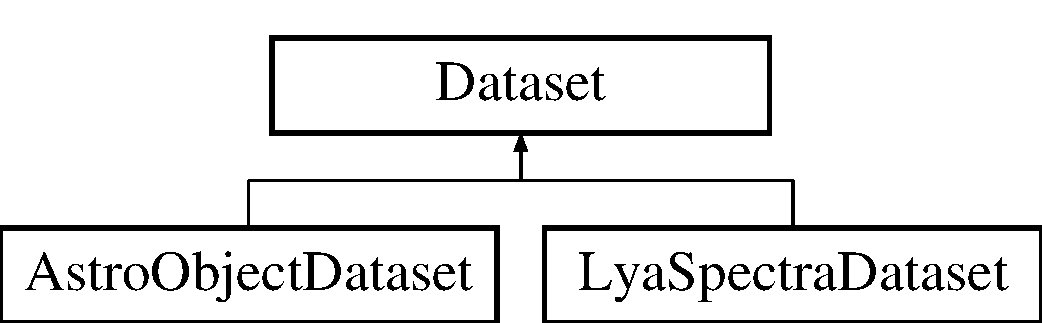
\includegraphics[height=2.000000cm]{class_dataset}
\end{center}
\end{figure}
\subsection*{Public Member Functions}
\begin{DoxyCompactItemize}
\item 
std\-::string \hyperlink{class_dataset_a7cacad140eadb450c4a0d6b1a9cd9ed0}{name} () const 
\item 
\hyperlink{struct_plates_map_simple}{Plates\-Map\-Simple}$<$ size\-\_\-t $>$\-::map \hyperlink{class_dataset_ab71a9a9e09ab029e37a7a69dbee63f2f}{num\-\_\-objects\-\_\-in\-\_\-plate} () const 
\item 
size\-\_\-t \hyperlink{class_dataset_a6b1f378ed9e786c2c7f60a82e4bbc834}{num\-\_\-objects\-\_\-in\-\_\-plate} (int plate\-\_\-number) const 
\item 
size\-\_\-t \hyperlink{class_dataset_ab28cc36ef5e2b5ba5fd055ba7d113c6d}{size} () const 
\item 
virtual void \hyperlink{class_dataset_a5867a14c1554b50ce062bdacd36460af}{Give\-R\-A\-D\-E\-C} (std\-::ostream \&out) const =0
\item 
virtual void \hyperlink{class_dataset_aae82d78ec374da243c22a96236b39465}{Give\-Z} (std\-::ostream \&out) const =0
\item 
virtual void \hyperlink{class_dataset_a76dbae8574850da55a3b88149ccbe3f9}{Set\-Distances} (const \hyperlink{class_interpolation_map}{Interpolation\-Map} \&redshift\-\_\-distance\-\_\-map)=0
\end{DoxyCompactItemize}
\subsection*{Protected Attributes}
\begin{DoxyCompactItemize}
\item 
std\-::string \hyperlink{class_dataset_a9e8765235cb821f6c4a43927aa60be9c}{name\-\_\-}
\item 
\hyperlink{struct_plates_map_simple}{Plates\-Map\-Simple}$<$ size\-\_\-t $>$\-::map \hyperlink{class_dataset_a42126d88c2da9941a94857fdd47f4186}{num\-\_\-objects\-\_\-in\-\_\-plate\-\_\-}
\item 
size\-\_\-t \hyperlink{class_dataset_aa9b7df288645726976e883b45180d84d}{size\-\_\-}
\end{DoxyCompactItemize}


\subsection{Detailed Description}
\hyperlink{dataset_8h}{dataset.\-h} Purpose\-: This file defines the class \hyperlink{class_dataset}{Dataset}. This class contains the variables necessary to store a dataset

\begin{DoxyAuthor}{Author}
Ignasi Pérez-\/\-Ràfols (\href{mailto:iprafols@icc.ub.edu}{\tt iprafols@icc.\-ub.\-edu}) 
\end{DoxyAuthor}
\begin{DoxyVersion}{Version}
1.\-0 07/25/2014 
\end{DoxyVersion}


Definition at line 29 of file dataset.\-h.



\subsection{Member Function Documentation}
\hypertarget{class_dataset_a5867a14c1554b50ce062bdacd36460af}{\index{Dataset@{Dataset}!Give\-R\-A\-D\-E\-C@{Give\-R\-A\-D\-E\-C}}
\index{Give\-R\-A\-D\-E\-C@{Give\-R\-A\-D\-E\-C}!Dataset@{Dataset}}
\subsubsection[{Give\-R\-A\-D\-E\-C}]{\setlength{\rightskip}{0pt plus 5cm}virtual void {\bf Dataset\-::\-Give\-R\-A\-D\-E\-C} (
\begin{DoxyParamCaption}
\item[{std\-::ostream \&}]{out}
\end{DoxyParamCaption}
) const\hspace{0.3cm}{\ttfamily  \mbox{[}pure virtual\mbox{]}}}}\label{class_dataset_a5867a14c1554b50ce062bdacd36460af}


Implemented in \hyperlink{class_astro_object_dataset_a6dbee08285bbd1fba5b900e637ce5b2d}{Astro\-Object\-Dataset}, and \hyperlink{class_lya_spectra_dataset_a29aa2c3f113d6cbc9d10bfabad12362d}{Lya\-Spectra\-Dataset}.

\hypertarget{class_dataset_aae82d78ec374da243c22a96236b39465}{\index{Dataset@{Dataset}!Give\-Z@{Give\-Z}}
\index{Give\-Z@{Give\-Z}!Dataset@{Dataset}}
\subsubsection[{Give\-Z}]{\setlength{\rightskip}{0pt plus 5cm}virtual void {\bf Dataset\-::\-Give\-Z} (
\begin{DoxyParamCaption}
\item[{std\-::ostream \&}]{out}
\end{DoxyParamCaption}
) const\hspace{0.3cm}{\ttfamily  \mbox{[}pure virtual\mbox{]}}}}\label{class_dataset_aae82d78ec374da243c22a96236b39465}


Implemented in \hyperlink{class_astro_object_dataset_a98c5a1ebf074c2589ed1e924bf5899bc}{Astro\-Object\-Dataset}, and \hyperlink{class_lya_spectra_dataset_a859711c028a33cf935ca5a5a3fb480fd}{Lya\-Spectra\-Dataset}.

\hypertarget{class_dataset_a7cacad140eadb450c4a0d6b1a9cd9ed0}{\index{Dataset@{Dataset}!name@{name}}
\index{name@{name}!Dataset@{Dataset}}
\subsubsection[{name}]{\setlength{\rightskip}{0pt plus 5cm}std\-::string {\bf Dataset\-::name} (
\begin{DoxyParamCaption}
{}
\end{DoxyParamCaption}
) const\hspace{0.3cm}{\ttfamily  \mbox{[}inline\mbox{]}}}}\label{class_dataset_a7cacad140eadb450c4a0d6b1a9cd9ed0}


Definition at line 37 of file dataset.\-h.


\begin{DoxyCode}
{return name_;}
\end{DoxyCode}
\hypertarget{class_dataset_ab71a9a9e09ab029e37a7a69dbee63f2f}{\index{Dataset@{Dataset}!num\-\_\-objects\-\_\-in\-\_\-plate@{num\-\_\-objects\-\_\-in\-\_\-plate}}
\index{num\-\_\-objects\-\_\-in\-\_\-plate@{num\-\_\-objects\-\_\-in\-\_\-plate}!Dataset@{Dataset}}
\subsubsection[{num\-\_\-objects\-\_\-in\-\_\-plate}]{\setlength{\rightskip}{0pt plus 5cm}{\bf Plates\-Map\-Simple}$<$size\-\_\-t$>$\-::map {\bf Dataset\-::num\-\_\-objects\-\_\-in\-\_\-plate} (
\begin{DoxyParamCaption}
{}
\end{DoxyParamCaption}
) const\hspace{0.3cm}{\ttfamily  \mbox{[}inline\mbox{]}}}}\label{class_dataset_ab71a9a9e09ab029e37a7a69dbee63f2f}


Definition at line 40 of file dataset.\-h.


\begin{DoxyCode}
{return num_objects_in_plate_;}
\end{DoxyCode}
\hypertarget{class_dataset_a6b1f378ed9e786c2c7f60a82e4bbc834}{\index{Dataset@{Dataset}!num\-\_\-objects\-\_\-in\-\_\-plate@{num\-\_\-objects\-\_\-in\-\_\-plate}}
\index{num\-\_\-objects\-\_\-in\-\_\-plate@{num\-\_\-objects\-\_\-in\-\_\-plate}!Dataset@{Dataset}}
\subsubsection[{num\-\_\-objects\-\_\-in\-\_\-plate}]{\setlength{\rightskip}{0pt plus 5cm}size\-\_\-t {\bf Dataset\-::num\-\_\-objects\-\_\-in\-\_\-plate} (
\begin{DoxyParamCaption}
\item[{int}]{plate\-\_\-number}
\end{DoxyParamCaption}
) const\hspace{0.3cm}{\ttfamily  \mbox{[}inline\mbox{]}}}}\label{class_dataset_a6b1f378ed9e786c2c7f60a82e4bbc834}


Definition at line 41 of file dataset.\-h.


\begin{DoxyCode}
{return (*num_objects_in_plate_.find(plate_number)).second;}
\end{DoxyCode}
\hypertarget{class_dataset_a76dbae8574850da55a3b88149ccbe3f9}{\index{Dataset@{Dataset}!Set\-Distances@{Set\-Distances}}
\index{Set\-Distances@{Set\-Distances}!Dataset@{Dataset}}
\subsubsection[{Set\-Distances}]{\setlength{\rightskip}{0pt plus 5cm}virtual void {\bf Dataset\-::\-Set\-Distances} (
\begin{DoxyParamCaption}
\item[{const {\bf Interpolation\-Map} \&}]{redshift\-\_\-distance\-\_\-map}
\end{DoxyParamCaption}
)\hspace{0.3cm}{\ttfamily  \mbox{[}pure virtual\mbox{]}}}}\label{class_dataset_a76dbae8574850da55a3b88149ccbe3f9}


Implemented in \hyperlink{class_astro_object_dataset_a4fe526d8aaf1f7e0182d5f30f82dcc60}{Astro\-Object\-Dataset}, and \hyperlink{class_lya_spectra_dataset_a444d22db8e799457aef351e74107802e}{Lya\-Spectra\-Dataset}.

\hypertarget{class_dataset_ab28cc36ef5e2b5ba5fd055ba7d113c6d}{\index{Dataset@{Dataset}!size@{size}}
\index{size@{size}!Dataset@{Dataset}}
\subsubsection[{size}]{\setlength{\rightskip}{0pt plus 5cm}size\-\_\-t {\bf Dataset\-::size} (
\begin{DoxyParamCaption}
{}
\end{DoxyParamCaption}
) const\hspace{0.3cm}{\ttfamily  \mbox{[}inline\mbox{]}}}}\label{class_dataset_ab28cc36ef5e2b5ba5fd055ba7d113c6d}


Definition at line 44 of file dataset.\-h.


\begin{DoxyCode}
{return size_;}
\end{DoxyCode}


\subsection{Member Data Documentation}
\hypertarget{class_dataset_a9e8765235cb821f6c4a43927aa60be9c}{\index{Dataset@{Dataset}!name\-\_\-@{name\-\_\-}}
\index{name\-\_\-@{name\-\_\-}!Dataset@{Dataset}}
\subsubsection[{name\-\_\-}]{\setlength{\rightskip}{0pt plus 5cm}std\-::string {\bf Dataset\-::name\-\_\-}\hspace{0.3cm}{\ttfamily  \mbox{[}protected\mbox{]}}}}\label{class_dataset_a9e8765235cb821f6c4a43927aa60be9c}


Definition at line 62 of file dataset.\-h.

\hypertarget{class_dataset_a42126d88c2da9941a94857fdd47f4186}{\index{Dataset@{Dataset}!num\-\_\-objects\-\_\-in\-\_\-plate\-\_\-@{num\-\_\-objects\-\_\-in\-\_\-plate\-\_\-}}
\index{num\-\_\-objects\-\_\-in\-\_\-plate\-\_\-@{num\-\_\-objects\-\_\-in\-\_\-plate\-\_\-}!Dataset@{Dataset}}
\subsubsection[{num\-\_\-objects\-\_\-in\-\_\-plate\-\_\-}]{\setlength{\rightskip}{0pt plus 5cm}{\bf Plates\-Map\-Simple}$<$size\-\_\-t$>$\-::map {\bf Dataset\-::num\-\_\-objects\-\_\-in\-\_\-plate\-\_\-}\hspace{0.3cm}{\ttfamily  \mbox{[}protected\mbox{]}}}}\label{class_dataset_a42126d88c2da9941a94857fdd47f4186}


Definition at line 65 of file dataset.\-h.

\hypertarget{class_dataset_aa9b7df288645726976e883b45180d84d}{\index{Dataset@{Dataset}!size\-\_\-@{size\-\_\-}}
\index{size\-\_\-@{size\-\_\-}!Dataset@{Dataset}}
\subsubsection[{size\-\_\-}]{\setlength{\rightskip}{0pt plus 5cm}size\-\_\-t {\bf Dataset\-::size\-\_\-}\hspace{0.3cm}{\ttfamily  \mbox{[}protected\mbox{]}}}}\label{class_dataset_aa9b7df288645726976e883b45180d84d}


Definition at line 68 of file dataset.\-h.



The documentation for this class was generated from the following file\-:\begin{DoxyCompactItemize}
\item 
\hyperlink{dataset_8h}{dataset.\-h}\end{DoxyCompactItemize}

\hypertarget{class_global_variables}{\section{Global\-Variables Class Reference}
\label{class_global_variables}\index{Global\-Variables@{Global\-Variables}}
}


{\ttfamily \#include $<$global\-\_\-variables.\-h$>$}

\subsection*{Public Member Functions}
\begin{DoxyCompactItemize}
\item 
\hyperlink{class_global_variables_a4631d1ecf5fe11e440926a3464028eb0}{Global\-Variables} ()
\item 
double \hyperlink{class_global_variables_aa30e576f3563c41b63177a5ae93b9aab}{c} () const 
\item 
std\-::string \hyperlink{class_global_variables_ab8932c7446ddcc1bbf9f19d07ec44424}{correlation\-\_\-file\-\_\-name} () const 
\item 
double \hyperlink{class_global_variables_ab5102be8fa70c050ab20349e47fa388d}{h} () const 
\item 
double \hyperlink{class_global_variables_a1ae6b307005b7da0849b79173ab5b62d}{h0} () const 
\item 
std\-::string \hyperlink{class_global_variables_a7b251a0da7026b671d8a68279cab4ae7}{lya\-\_\-spectra\-\_\-catalog} () const 
\item 
std\-::string \hyperlink{class_global_variables_a7ef593cd3a148af75812f2e8479595ae}{lya\-\_\-spectra\-\_\-catalog\-\_\-name} () const 
\item 
std\-::string \hyperlink{class_global_variables_ac337ea3586fbb1346240ad25c696f6f0}{lya\-\_\-spectra\-\_\-dir} () const 
\item 
double \hyperlink{class_global_variables_a2893eb2c29a895d604ac471c320f4a39}{lya\-\_\-wl} () const 
\item 
double \hyperlink{class_global_variables_ae3688afd60bb03fd4e788d27af1ac8fe}{max\-\_\-pi} () const 
\item 
double \hyperlink{class_global_variables_a13694704b2bb849bae0d46e577246fb0}{max\-\_\-sigma} () const 
\item 
double \hyperlink{class_global_variables_aae93df7713a9e59706c8d8cd03e62a8a}{neighbours\-\_\-max\-\_\-distance} () const 
\item 
std\-::string \hyperlink{class_global_variables_a7481f788f94ed1bdb590057d7a0f48ca}{normalized\-\_\-correlation} () const 
\item 
int \hyperlink{class_global_variables_a8df4bf4e1962af98f59cd43947188509}{num\-\_\-bins} () const 
\item 
int \hyperlink{class_global_variables_a08ee1fac0ba1c1eccb8fd405c1f9cb1c}{num\-\_\-pi\-\_\-bins} () const 
\item 
int \hyperlink{class_global_variables_a09a6fd5da6b9c5a3a9aa63bee7e4466f}{num\-\_\-plates} () const 
\item 
int \hyperlink{class_global_variables_a054d4cf825a69d3461475a3590799774}{num\-\_\-points\-\_\-interpolation} () const 
\item 
int \hyperlink{class_global_variables_a5ccd02c696d64e9c33fc6a7e1ba8b9ef}{num\-\_\-sigma\-\_\-bins} () const 
\item 
std\-::string \hyperlink{class_global_variables_ab3641ef310a60651c562a7dc8864d0e9}{objects\-\_\-catalog} () const 
\item 
std\-::string \hyperlink{class_global_variables_a8412ac07504633c4abd23702b4d4d823}{objects\-\_\-catalog\-\_\-name} () const 
\item 
std\-::string \hyperlink{class_global_variables_ac10711bcd7293ce5da996b4f5b79de2b}{pairs\-\_\-file\-\_\-name} () const 
\item 
std\-::string \hyperlink{class_global_variables_abf1a6505c3dab27b4dc58fc1634e70e7}{plate\-\_\-neighbours} () const 
\item 
std\-::string \hyperlink{class_global_variables_a825d2ce1a68bbdca6395aa10690e3407}{plots} () const 
\item 
std\-::string \hyperlink{class_global_variables_a03e3e8cbe112ab714544e57f541a693f}{pwd} () const 
\item 
std\-::string \hyperlink{class_global_variables_a53b4346935148918029cc1a2daaad80c}{results} () const 
\item 
double \hyperlink{class_global_variables_aba979c1ae01246184e65e4034007f0ca}{step\-\_\-pi} () const 
\item 
double \hyperlink{class_global_variables_a0a1e6c768c7323c1da081db7c375060e}{step\-\_\-sigma} () const 
\item 
double \hyperlink{class_global_variables_ae01eadf8a6614c2b8f5e5a5da5b0a7c3}{wm} () const 
\item 
double \hyperlink{class_global_variables_a09e2005546be6c1147d898fbd9f040e0}{z\-\_\-max} () const 
\item 
double \hyperlink{class_global_variables_ad2dee77ee4d577e3a9575184089735ac}{z\-\_\-max\-\_\-interpolation} () const 
\item 
double \hyperlink{class_global_variables_ac6ed0b46b3ab483ba201b193b0953905}{z\-\_\-min} () const 
\item 
double \hyperlink{class_global_variables_a3f167911da6733d4f4ebf58949d24c02}{z\-\_\-min\-\_\-interpolation} () const 
\end{DoxyCompactItemize}


\subsection{Detailed Description}
global \-\_\-variables.\-h Purpose\-: This file defines the class \hyperlink{class_global_variables}{Global\-Variables}. This class contains the constant variables which are used in a \char`\"{}global\char`\"{} sense

\begin{DoxyAuthor}{Author}
Ignasi Pérez-\/\-Ràfols (\href{mailto:iprafols@icc.ub.edu}{\tt iprafols@icc.\-ub.\-edu}) 
\end{DoxyAuthor}
\begin{DoxyVersion}{Version}
1.\-0 on 17/06/14 
\end{DoxyVersion}


Definition at line 25 of file global\-\_\-variables.\-h.



\subsection{Constructor \& Destructor Documentation}
\hypertarget{class_global_variables_a4631d1ecf5fe11e440926a3464028eb0}{\index{Global\-Variables@{Global\-Variables}!Global\-Variables@{Global\-Variables}}
\index{Global\-Variables@{Global\-Variables}!GlobalVariables@{Global\-Variables}}
\subsubsection[{Global\-Variables}]{\setlength{\rightskip}{0pt plus 5cm}{\bf Global\-Variables\-::\-Global\-Variables} (
\begin{DoxyParamCaption}
{}
\end{DoxyParamCaption}
)}}\label{class_global_variables_a4631d1ecf5fe11e440926a3464028eb0}
\hyperlink{global__variables_8cpp}{global\-\_\-variables.\-cpp} Purpose\-: This files contains the body for the functions defined in \hyperlink{global__variables_8h}{global\-\_\-variables.\-h}

\begin{DoxyAuthor}{Author}
Ignasi Pérez-\/\-Ràfols 
\end{DoxyAuthor}
\begin{DoxyVersion}{Version}
1.\-0 06/17/2014 
\end{DoxyVersion}
E\-X\-P\-L\-A\-N\-A\-T\-I\-O\-N\-: Cosntructs a \hyperlink{class_global_variables}{Global\-Variables} instance and initializes all its variables

I\-N\-P\-U\-T\-S\-: N\-O\-N\-E

O\-U\-T\-P\-U\-T\-S\-: N\-O\-N\-E

C\-L\-A\-S\-S\-E\-S U\-S\-E\-D\-: \hyperlink{class_global_variables}{Global\-Variables}

F\-U\-N\-C\-I\-T\-O\-N\-S U\-S\-E\-D\-: N\-O\-N\-E

Definition at line 11 of file global\-\_\-variables.\-cpp.


\begin{DoxyCode}
                                {
    //
    // general settings
    //
    //pwd_ = "/Users/iprafols/cross_correlations/";
    pwd_ = "/triforce/iprafols/cross_correlations/";
    results_ = pwd_ + "results2/";
    plots_ = pwd_ + "plots2/";
    objects_catalog_ = pwd_ + "DR11Q_alpha_v0.fits";
    objects_catalog_name_ = "DR11Q_alpha_v0";
    pairs_file_name_ = "qso_spectrum_pairs_plate_";
    correlation_file_name_ = results_ + "correlation_bin_";
    normalized_correlation_ = results_ + "normalized_correlation.dat";
    plate_neighbours_ = pwd_ + "plate_neighbours.dat";
    lya_spectra_dir_ = pwd_ + "spectrum_fits_files/";
    //lya_spectra_catalog_ = pwd_ + "DR11Q_spectra_forest_one_spectrum.ls";//
       versió per fer proves
    lya_spectra_catalog_ = pwd_ + "DR11Q_spectra_forest_some_spectrum.ls";//
       versió per fer proves
    //lya_spectra_catalog_ = pwd_ + "DR11Q_spectra_forest_list.ls"; // versió
       definitiva
    lya_spectra_catalog_name_ = "DR11Q_spectra_forest";
    num_plates_ = 2044; // DR11
    
    //
    // Fidutial model
    //
    h0_ = 68.0;
    h_ = h0_/100.0;
    wm_ = 0.3;
    
    //
    // bin setting
    //
    neighbours_max_distance_ = 3.0*acos(-1.0)/180.0; // (in radians)
    max_pi_ = 50.0; // (in Mpc/h)
    max_sigma_ = 50.0; // (in Mpc/h)
    step_pi_ = 5.0; // (in Mpc/h)
    step_sigma_ = 5.0; // (in Mpc/h)
    num_pi_bins_ = int(2.0*max_pi_/step_pi_);
    num_sigma_bins_ = int(max_sigma_/step_sigma_);
    num_bins_ = num_pi_bins_*num_sigma_bins_;
    
    //
    // line and redshift settings
    //
    lya_wl_ = 1215.67;
    z_min_ = 2.0;
    z_max_ = 3.5;
    z_min_interpolation_ = 1.5; 
    z_max_interpolation_ = 4.0; 
    num_points_interpolation_ = 30000; 
    
    //
    // Some mathematical and physical constants
    //
    c_ = 299792.458;
}\end{DoxyCode}


\subsection{Member Function Documentation}
\hypertarget{class_global_variables_aa30e576f3563c41b63177a5ae93b9aab}{\index{Global\-Variables@{Global\-Variables}!c@{c}}
\index{c@{c}!GlobalVariables@{Global\-Variables}}
\subsubsection[{c}]{\setlength{\rightskip}{0pt plus 5cm}double {\bf Global\-Variables\-::c} (
\begin{DoxyParamCaption}
{}
\end{DoxyParamCaption}
) const\hspace{0.3cm}{\ttfamily  \mbox{[}inline\mbox{]}}}}\label{class_global_variables_aa30e576f3563c41b63177a5ae93b9aab}


Definition at line 38 of file global\-\_\-variables.\-h.


\begin{DoxyCode}
{return c_;}
\end{DoxyCode}
\hypertarget{class_global_variables_ab8932c7446ddcc1bbf9f19d07ec44424}{\index{Global\-Variables@{Global\-Variables}!correlation\-\_\-file\-\_\-name@{correlation\-\_\-file\-\_\-name}}
\index{correlation\-\_\-file\-\_\-name@{correlation\-\_\-file\-\_\-name}!GlobalVariables@{Global\-Variables}}
\subsubsection[{correlation\-\_\-file\-\_\-name}]{\setlength{\rightskip}{0pt plus 5cm}std\-::string {\bf Global\-Variables\-::correlation\-\_\-file\-\_\-name} (
\begin{DoxyParamCaption}
{}
\end{DoxyParamCaption}
) const\hspace{0.3cm}{\ttfamily  \mbox{[}inline\mbox{]}}}}\label{class_global_variables_ab8932c7446ddcc1bbf9f19d07ec44424}


Definition at line 41 of file global\-\_\-variables.\-h.


\begin{DoxyCode}
{return correlation_file_name_;}
\end{DoxyCode}
\hypertarget{class_global_variables_ab5102be8fa70c050ab20349e47fa388d}{\index{Global\-Variables@{Global\-Variables}!h@{h}}
\index{h@{h}!GlobalVariables@{Global\-Variables}}
\subsubsection[{h}]{\setlength{\rightskip}{0pt plus 5cm}double {\bf Global\-Variables\-::h} (
\begin{DoxyParamCaption}
{}
\end{DoxyParamCaption}
) const\hspace{0.3cm}{\ttfamily  \mbox{[}inline\mbox{]}}}}\label{class_global_variables_ab5102be8fa70c050ab20349e47fa388d}


Definition at line 44 of file global\-\_\-variables.\-h.


\begin{DoxyCode}
{return h_;}
\end{DoxyCode}
\hypertarget{class_global_variables_a1ae6b307005b7da0849b79173ab5b62d}{\index{Global\-Variables@{Global\-Variables}!h0@{h0}}
\index{h0@{h0}!GlobalVariables@{Global\-Variables}}
\subsubsection[{h0}]{\setlength{\rightskip}{0pt plus 5cm}double {\bf Global\-Variables\-::h0} (
\begin{DoxyParamCaption}
{}
\end{DoxyParamCaption}
) const\hspace{0.3cm}{\ttfamily  \mbox{[}inline\mbox{]}}}}\label{class_global_variables_a1ae6b307005b7da0849b79173ab5b62d}


Definition at line 47 of file global\-\_\-variables.\-h.


\begin{DoxyCode}
{return h0_;}
\end{DoxyCode}
\hypertarget{class_global_variables_a7b251a0da7026b671d8a68279cab4ae7}{\index{Global\-Variables@{Global\-Variables}!lya\-\_\-spectra\-\_\-catalog@{lya\-\_\-spectra\-\_\-catalog}}
\index{lya\-\_\-spectra\-\_\-catalog@{lya\-\_\-spectra\-\_\-catalog}!GlobalVariables@{Global\-Variables}}
\subsubsection[{lya\-\_\-spectra\-\_\-catalog}]{\setlength{\rightskip}{0pt plus 5cm}std\-::string {\bf Global\-Variables\-::lya\-\_\-spectra\-\_\-catalog} (
\begin{DoxyParamCaption}
{}
\end{DoxyParamCaption}
) const\hspace{0.3cm}{\ttfamily  \mbox{[}inline\mbox{]}}}}\label{class_global_variables_a7b251a0da7026b671d8a68279cab4ae7}


Definition at line 50 of file global\-\_\-variables.\-h.


\begin{DoxyCode}
{return lya_spectra_catalog_;}
\end{DoxyCode}
\hypertarget{class_global_variables_a7ef593cd3a148af75812f2e8479595ae}{\index{Global\-Variables@{Global\-Variables}!lya\-\_\-spectra\-\_\-catalog\-\_\-name@{lya\-\_\-spectra\-\_\-catalog\-\_\-name}}
\index{lya\-\_\-spectra\-\_\-catalog\-\_\-name@{lya\-\_\-spectra\-\_\-catalog\-\_\-name}!GlobalVariables@{Global\-Variables}}
\subsubsection[{lya\-\_\-spectra\-\_\-catalog\-\_\-name}]{\setlength{\rightskip}{0pt plus 5cm}std\-::string {\bf Global\-Variables\-::lya\-\_\-spectra\-\_\-catalog\-\_\-name} (
\begin{DoxyParamCaption}
{}
\end{DoxyParamCaption}
) const\hspace{0.3cm}{\ttfamily  \mbox{[}inline\mbox{]}}}}\label{class_global_variables_a7ef593cd3a148af75812f2e8479595ae}


Definition at line 53 of file global\-\_\-variables.\-h.


\begin{DoxyCode}
{return lya_spectra_catalog_name_;}
\end{DoxyCode}
\hypertarget{class_global_variables_ac337ea3586fbb1346240ad25c696f6f0}{\index{Global\-Variables@{Global\-Variables}!lya\-\_\-spectra\-\_\-dir@{lya\-\_\-spectra\-\_\-dir}}
\index{lya\-\_\-spectra\-\_\-dir@{lya\-\_\-spectra\-\_\-dir}!GlobalVariables@{Global\-Variables}}
\subsubsection[{lya\-\_\-spectra\-\_\-dir}]{\setlength{\rightskip}{0pt plus 5cm}std\-::string {\bf Global\-Variables\-::lya\-\_\-spectra\-\_\-dir} (
\begin{DoxyParamCaption}
{}
\end{DoxyParamCaption}
) const\hspace{0.3cm}{\ttfamily  \mbox{[}inline\mbox{]}}}}\label{class_global_variables_ac337ea3586fbb1346240ad25c696f6f0}


Definition at line 56 of file global\-\_\-variables.\-h.


\begin{DoxyCode}
{return lya_spectra_dir_;}
\end{DoxyCode}
\hypertarget{class_global_variables_a2893eb2c29a895d604ac471c320f4a39}{\index{Global\-Variables@{Global\-Variables}!lya\-\_\-wl@{lya\-\_\-wl}}
\index{lya\-\_\-wl@{lya\-\_\-wl}!GlobalVariables@{Global\-Variables}}
\subsubsection[{lya\-\_\-wl}]{\setlength{\rightskip}{0pt plus 5cm}double {\bf Global\-Variables\-::lya\-\_\-wl} (
\begin{DoxyParamCaption}
{}
\end{DoxyParamCaption}
) const\hspace{0.3cm}{\ttfamily  \mbox{[}inline\mbox{]}}}}\label{class_global_variables_a2893eb2c29a895d604ac471c320f4a39}


Definition at line 59 of file global\-\_\-variables.\-h.


\begin{DoxyCode}
{return lya_wl_;}
\end{DoxyCode}
\hypertarget{class_global_variables_ae3688afd60bb03fd4e788d27af1ac8fe}{\index{Global\-Variables@{Global\-Variables}!max\-\_\-pi@{max\-\_\-pi}}
\index{max\-\_\-pi@{max\-\_\-pi}!GlobalVariables@{Global\-Variables}}
\subsubsection[{max\-\_\-pi}]{\setlength{\rightskip}{0pt plus 5cm}double {\bf Global\-Variables\-::max\-\_\-pi} (
\begin{DoxyParamCaption}
{}
\end{DoxyParamCaption}
) const\hspace{0.3cm}{\ttfamily  \mbox{[}inline\mbox{]}}}}\label{class_global_variables_ae3688afd60bb03fd4e788d27af1ac8fe}


Definition at line 62 of file global\-\_\-variables.\-h.


\begin{DoxyCode}
{return max_pi_;}
\end{DoxyCode}
\hypertarget{class_global_variables_a13694704b2bb849bae0d46e577246fb0}{\index{Global\-Variables@{Global\-Variables}!max\-\_\-sigma@{max\-\_\-sigma}}
\index{max\-\_\-sigma@{max\-\_\-sigma}!GlobalVariables@{Global\-Variables}}
\subsubsection[{max\-\_\-sigma}]{\setlength{\rightskip}{0pt plus 5cm}double {\bf Global\-Variables\-::max\-\_\-sigma} (
\begin{DoxyParamCaption}
{}
\end{DoxyParamCaption}
) const\hspace{0.3cm}{\ttfamily  \mbox{[}inline\mbox{]}}}}\label{class_global_variables_a13694704b2bb849bae0d46e577246fb0}


Definition at line 65 of file global\-\_\-variables.\-h.


\begin{DoxyCode}
{return max_sigma_;}
\end{DoxyCode}
\hypertarget{class_global_variables_aae93df7713a9e59706c8d8cd03e62a8a}{\index{Global\-Variables@{Global\-Variables}!neighbours\-\_\-max\-\_\-distance@{neighbours\-\_\-max\-\_\-distance}}
\index{neighbours\-\_\-max\-\_\-distance@{neighbours\-\_\-max\-\_\-distance}!GlobalVariables@{Global\-Variables}}
\subsubsection[{neighbours\-\_\-max\-\_\-distance}]{\setlength{\rightskip}{0pt plus 5cm}double {\bf Global\-Variables\-::neighbours\-\_\-max\-\_\-distance} (
\begin{DoxyParamCaption}
{}
\end{DoxyParamCaption}
) const\hspace{0.3cm}{\ttfamily  \mbox{[}inline\mbox{]}}}}\label{class_global_variables_aae93df7713a9e59706c8d8cd03e62a8a}


Definition at line 68 of file global\-\_\-variables.\-h.


\begin{DoxyCode}
{return neighbours_max_distance_;}
\end{DoxyCode}
\hypertarget{class_global_variables_a7481f788f94ed1bdb590057d7a0f48ca}{\index{Global\-Variables@{Global\-Variables}!normalized\-\_\-correlation@{normalized\-\_\-correlation}}
\index{normalized\-\_\-correlation@{normalized\-\_\-correlation}!GlobalVariables@{Global\-Variables}}
\subsubsection[{normalized\-\_\-correlation}]{\setlength{\rightskip}{0pt plus 5cm}std\-::string {\bf Global\-Variables\-::normalized\-\_\-correlation} (
\begin{DoxyParamCaption}
{}
\end{DoxyParamCaption}
) const\hspace{0.3cm}{\ttfamily  \mbox{[}inline\mbox{]}}}}\label{class_global_variables_a7481f788f94ed1bdb590057d7a0f48ca}


Definition at line 71 of file global\-\_\-variables.\-h.


\begin{DoxyCode}
{return normalized_correlation_;}
\end{DoxyCode}
\hypertarget{class_global_variables_a8df4bf4e1962af98f59cd43947188509}{\index{Global\-Variables@{Global\-Variables}!num\-\_\-bins@{num\-\_\-bins}}
\index{num\-\_\-bins@{num\-\_\-bins}!GlobalVariables@{Global\-Variables}}
\subsubsection[{num\-\_\-bins}]{\setlength{\rightskip}{0pt plus 5cm}int {\bf Global\-Variables\-::num\-\_\-bins} (
\begin{DoxyParamCaption}
{}
\end{DoxyParamCaption}
) const\hspace{0.3cm}{\ttfamily  \mbox{[}inline\mbox{]}}}}\label{class_global_variables_a8df4bf4e1962af98f59cd43947188509}


Definition at line 74 of file global\-\_\-variables.\-h.


\begin{DoxyCode}
{return num_bins_;}
\end{DoxyCode}
\hypertarget{class_global_variables_a08ee1fac0ba1c1eccb8fd405c1f9cb1c}{\index{Global\-Variables@{Global\-Variables}!num\-\_\-pi\-\_\-bins@{num\-\_\-pi\-\_\-bins}}
\index{num\-\_\-pi\-\_\-bins@{num\-\_\-pi\-\_\-bins}!GlobalVariables@{Global\-Variables}}
\subsubsection[{num\-\_\-pi\-\_\-bins}]{\setlength{\rightskip}{0pt plus 5cm}int {\bf Global\-Variables\-::num\-\_\-pi\-\_\-bins} (
\begin{DoxyParamCaption}
{}
\end{DoxyParamCaption}
) const\hspace{0.3cm}{\ttfamily  \mbox{[}inline\mbox{]}}}}\label{class_global_variables_a08ee1fac0ba1c1eccb8fd405c1f9cb1c}


Definition at line 77 of file global\-\_\-variables.\-h.


\begin{DoxyCode}
{return num_pi_bins_;}
\end{DoxyCode}
\hypertarget{class_global_variables_a09a6fd5da6b9c5a3a9aa63bee7e4466f}{\index{Global\-Variables@{Global\-Variables}!num\-\_\-plates@{num\-\_\-plates}}
\index{num\-\_\-plates@{num\-\_\-plates}!GlobalVariables@{Global\-Variables}}
\subsubsection[{num\-\_\-plates}]{\setlength{\rightskip}{0pt plus 5cm}int {\bf Global\-Variables\-::num\-\_\-plates} (
\begin{DoxyParamCaption}
{}
\end{DoxyParamCaption}
) const\hspace{0.3cm}{\ttfamily  \mbox{[}inline\mbox{]}}}}\label{class_global_variables_a09a6fd5da6b9c5a3a9aa63bee7e4466f}


Definition at line 80 of file global\-\_\-variables.\-h.


\begin{DoxyCode}
{return num_plates_;}
\end{DoxyCode}
\hypertarget{class_global_variables_a054d4cf825a69d3461475a3590799774}{\index{Global\-Variables@{Global\-Variables}!num\-\_\-points\-\_\-interpolation@{num\-\_\-points\-\_\-interpolation}}
\index{num\-\_\-points\-\_\-interpolation@{num\-\_\-points\-\_\-interpolation}!GlobalVariables@{Global\-Variables}}
\subsubsection[{num\-\_\-points\-\_\-interpolation}]{\setlength{\rightskip}{0pt plus 5cm}int {\bf Global\-Variables\-::num\-\_\-points\-\_\-interpolation} (
\begin{DoxyParamCaption}
{}
\end{DoxyParamCaption}
) const\hspace{0.3cm}{\ttfamily  \mbox{[}inline\mbox{]}}}}\label{class_global_variables_a054d4cf825a69d3461475a3590799774}


Definition at line 83 of file global\-\_\-variables.\-h.


\begin{DoxyCode}
{return num_points_interpolation_;}
\end{DoxyCode}
\hypertarget{class_global_variables_a5ccd02c696d64e9c33fc6a7e1ba8b9ef}{\index{Global\-Variables@{Global\-Variables}!num\-\_\-sigma\-\_\-bins@{num\-\_\-sigma\-\_\-bins}}
\index{num\-\_\-sigma\-\_\-bins@{num\-\_\-sigma\-\_\-bins}!GlobalVariables@{Global\-Variables}}
\subsubsection[{num\-\_\-sigma\-\_\-bins}]{\setlength{\rightskip}{0pt plus 5cm}int {\bf Global\-Variables\-::num\-\_\-sigma\-\_\-bins} (
\begin{DoxyParamCaption}
{}
\end{DoxyParamCaption}
) const\hspace{0.3cm}{\ttfamily  \mbox{[}inline\mbox{]}}}}\label{class_global_variables_a5ccd02c696d64e9c33fc6a7e1ba8b9ef}


Definition at line 86 of file global\-\_\-variables.\-h.


\begin{DoxyCode}
{return num_sigma_bins_;}
\end{DoxyCode}
\hypertarget{class_global_variables_ab3641ef310a60651c562a7dc8864d0e9}{\index{Global\-Variables@{Global\-Variables}!objects\-\_\-catalog@{objects\-\_\-catalog}}
\index{objects\-\_\-catalog@{objects\-\_\-catalog}!GlobalVariables@{Global\-Variables}}
\subsubsection[{objects\-\_\-catalog}]{\setlength{\rightskip}{0pt plus 5cm}std\-::string {\bf Global\-Variables\-::objects\-\_\-catalog} (
\begin{DoxyParamCaption}
{}
\end{DoxyParamCaption}
) const\hspace{0.3cm}{\ttfamily  \mbox{[}inline\mbox{]}}}}\label{class_global_variables_ab3641ef310a60651c562a7dc8864d0e9}


Definition at line 89 of file global\-\_\-variables.\-h.


\begin{DoxyCode}
{return objects_catalog_;}
\end{DoxyCode}
\hypertarget{class_global_variables_a8412ac07504633c4abd23702b4d4d823}{\index{Global\-Variables@{Global\-Variables}!objects\-\_\-catalog\-\_\-name@{objects\-\_\-catalog\-\_\-name}}
\index{objects\-\_\-catalog\-\_\-name@{objects\-\_\-catalog\-\_\-name}!GlobalVariables@{Global\-Variables}}
\subsubsection[{objects\-\_\-catalog\-\_\-name}]{\setlength{\rightskip}{0pt plus 5cm}std\-::string {\bf Global\-Variables\-::objects\-\_\-catalog\-\_\-name} (
\begin{DoxyParamCaption}
{}
\end{DoxyParamCaption}
) const\hspace{0.3cm}{\ttfamily  \mbox{[}inline\mbox{]}}}}\label{class_global_variables_a8412ac07504633c4abd23702b4d4d823}


Definition at line 92 of file global\-\_\-variables.\-h.


\begin{DoxyCode}
{return objects_catalog_name_;}
\end{DoxyCode}
\hypertarget{class_global_variables_ac10711bcd7293ce5da996b4f5b79de2b}{\index{Global\-Variables@{Global\-Variables}!pairs\-\_\-file\-\_\-name@{pairs\-\_\-file\-\_\-name}}
\index{pairs\-\_\-file\-\_\-name@{pairs\-\_\-file\-\_\-name}!GlobalVariables@{Global\-Variables}}
\subsubsection[{pairs\-\_\-file\-\_\-name}]{\setlength{\rightskip}{0pt plus 5cm}std\-::string {\bf Global\-Variables\-::pairs\-\_\-file\-\_\-name} (
\begin{DoxyParamCaption}
{}
\end{DoxyParamCaption}
) const\hspace{0.3cm}{\ttfamily  \mbox{[}inline\mbox{]}}}}\label{class_global_variables_ac10711bcd7293ce5da996b4f5b79de2b}


Definition at line 95 of file global\-\_\-variables.\-h.


\begin{DoxyCode}
{return pairs_file_name_;}
\end{DoxyCode}
\hypertarget{class_global_variables_abf1a6505c3dab27b4dc58fc1634e70e7}{\index{Global\-Variables@{Global\-Variables}!plate\-\_\-neighbours@{plate\-\_\-neighbours}}
\index{plate\-\_\-neighbours@{plate\-\_\-neighbours}!GlobalVariables@{Global\-Variables}}
\subsubsection[{plate\-\_\-neighbours}]{\setlength{\rightskip}{0pt plus 5cm}std\-::string {\bf Global\-Variables\-::plate\-\_\-neighbours} (
\begin{DoxyParamCaption}
{}
\end{DoxyParamCaption}
) const\hspace{0.3cm}{\ttfamily  \mbox{[}inline\mbox{]}}}}\label{class_global_variables_abf1a6505c3dab27b4dc58fc1634e70e7}


Definition at line 98 of file global\-\_\-variables.\-h.


\begin{DoxyCode}
{return plate_neighbours_;}
\end{DoxyCode}
\hypertarget{class_global_variables_a825d2ce1a68bbdca6395aa10690e3407}{\index{Global\-Variables@{Global\-Variables}!plots@{plots}}
\index{plots@{plots}!GlobalVariables@{Global\-Variables}}
\subsubsection[{plots}]{\setlength{\rightskip}{0pt plus 5cm}std\-::string {\bf Global\-Variables\-::plots} (
\begin{DoxyParamCaption}
{}
\end{DoxyParamCaption}
) const\hspace{0.3cm}{\ttfamily  \mbox{[}inline\mbox{]}}}}\label{class_global_variables_a825d2ce1a68bbdca6395aa10690e3407}


Definition at line 101 of file global\-\_\-variables.\-h.


\begin{DoxyCode}
{return plots_;}
\end{DoxyCode}
\hypertarget{class_global_variables_a03e3e8cbe112ab714544e57f541a693f}{\index{Global\-Variables@{Global\-Variables}!pwd@{pwd}}
\index{pwd@{pwd}!GlobalVariables@{Global\-Variables}}
\subsubsection[{pwd}]{\setlength{\rightskip}{0pt plus 5cm}std\-::string {\bf Global\-Variables\-::pwd} (
\begin{DoxyParamCaption}
{}
\end{DoxyParamCaption}
) const\hspace{0.3cm}{\ttfamily  \mbox{[}inline\mbox{]}}}}\label{class_global_variables_a03e3e8cbe112ab714544e57f541a693f}


Definition at line 104 of file global\-\_\-variables.\-h.


\begin{DoxyCode}
{return pwd_;}
\end{DoxyCode}
\hypertarget{class_global_variables_a53b4346935148918029cc1a2daaad80c}{\index{Global\-Variables@{Global\-Variables}!results@{results}}
\index{results@{results}!GlobalVariables@{Global\-Variables}}
\subsubsection[{results}]{\setlength{\rightskip}{0pt plus 5cm}std\-::string {\bf Global\-Variables\-::results} (
\begin{DoxyParamCaption}
{}
\end{DoxyParamCaption}
) const\hspace{0.3cm}{\ttfamily  \mbox{[}inline\mbox{]}}}}\label{class_global_variables_a53b4346935148918029cc1a2daaad80c}


Definition at line 107 of file global\-\_\-variables.\-h.


\begin{DoxyCode}
{return results_;}
\end{DoxyCode}
\hypertarget{class_global_variables_aba979c1ae01246184e65e4034007f0ca}{\index{Global\-Variables@{Global\-Variables}!step\-\_\-pi@{step\-\_\-pi}}
\index{step\-\_\-pi@{step\-\_\-pi}!GlobalVariables@{Global\-Variables}}
\subsubsection[{step\-\_\-pi}]{\setlength{\rightskip}{0pt plus 5cm}double {\bf Global\-Variables\-::step\-\_\-pi} (
\begin{DoxyParamCaption}
{}
\end{DoxyParamCaption}
) const\hspace{0.3cm}{\ttfamily  \mbox{[}inline\mbox{]}}}}\label{class_global_variables_aba979c1ae01246184e65e4034007f0ca}


Definition at line 110 of file global\-\_\-variables.\-h.


\begin{DoxyCode}
{return step_pi_;}
\end{DoxyCode}
\hypertarget{class_global_variables_a0a1e6c768c7323c1da081db7c375060e}{\index{Global\-Variables@{Global\-Variables}!step\-\_\-sigma@{step\-\_\-sigma}}
\index{step\-\_\-sigma@{step\-\_\-sigma}!GlobalVariables@{Global\-Variables}}
\subsubsection[{step\-\_\-sigma}]{\setlength{\rightskip}{0pt plus 5cm}double {\bf Global\-Variables\-::step\-\_\-sigma} (
\begin{DoxyParamCaption}
{}
\end{DoxyParamCaption}
) const\hspace{0.3cm}{\ttfamily  \mbox{[}inline\mbox{]}}}}\label{class_global_variables_a0a1e6c768c7323c1da081db7c375060e}


Definition at line 113 of file global\-\_\-variables.\-h.


\begin{DoxyCode}
{return step_sigma_;}
\end{DoxyCode}
\hypertarget{class_global_variables_ae01eadf8a6614c2b8f5e5a5da5b0a7c3}{\index{Global\-Variables@{Global\-Variables}!wm@{wm}}
\index{wm@{wm}!GlobalVariables@{Global\-Variables}}
\subsubsection[{wm}]{\setlength{\rightskip}{0pt plus 5cm}double {\bf Global\-Variables\-::wm} (
\begin{DoxyParamCaption}
{}
\end{DoxyParamCaption}
) const\hspace{0.3cm}{\ttfamily  \mbox{[}inline\mbox{]}}}}\label{class_global_variables_ae01eadf8a6614c2b8f5e5a5da5b0a7c3}


Definition at line 116 of file global\-\_\-variables.\-h.


\begin{DoxyCode}
{return wm_;}
\end{DoxyCode}
\hypertarget{class_global_variables_a09e2005546be6c1147d898fbd9f040e0}{\index{Global\-Variables@{Global\-Variables}!z\-\_\-max@{z\-\_\-max}}
\index{z\-\_\-max@{z\-\_\-max}!GlobalVariables@{Global\-Variables}}
\subsubsection[{z\-\_\-max}]{\setlength{\rightskip}{0pt plus 5cm}double {\bf Global\-Variables\-::z\-\_\-max} (
\begin{DoxyParamCaption}
{}
\end{DoxyParamCaption}
) const\hspace{0.3cm}{\ttfamily  \mbox{[}inline\mbox{]}}}}\label{class_global_variables_a09e2005546be6c1147d898fbd9f040e0}


Definition at line 119 of file global\-\_\-variables.\-h.


\begin{DoxyCode}
{return z_max_;}
\end{DoxyCode}
\hypertarget{class_global_variables_ad2dee77ee4d577e3a9575184089735ac}{\index{Global\-Variables@{Global\-Variables}!z\-\_\-max\-\_\-interpolation@{z\-\_\-max\-\_\-interpolation}}
\index{z\-\_\-max\-\_\-interpolation@{z\-\_\-max\-\_\-interpolation}!GlobalVariables@{Global\-Variables}}
\subsubsection[{z\-\_\-max\-\_\-interpolation}]{\setlength{\rightskip}{0pt plus 5cm}double {\bf Global\-Variables\-::z\-\_\-max\-\_\-interpolation} (
\begin{DoxyParamCaption}
{}
\end{DoxyParamCaption}
) const\hspace{0.3cm}{\ttfamily  \mbox{[}inline\mbox{]}}}}\label{class_global_variables_ad2dee77ee4d577e3a9575184089735ac}


Definition at line 122 of file global\-\_\-variables.\-h.


\begin{DoxyCode}
{return z_max_interpolation_;}
\end{DoxyCode}
\hypertarget{class_global_variables_ac6ed0b46b3ab483ba201b193b0953905}{\index{Global\-Variables@{Global\-Variables}!z\-\_\-min@{z\-\_\-min}}
\index{z\-\_\-min@{z\-\_\-min}!GlobalVariables@{Global\-Variables}}
\subsubsection[{z\-\_\-min}]{\setlength{\rightskip}{0pt plus 5cm}double {\bf Global\-Variables\-::z\-\_\-min} (
\begin{DoxyParamCaption}
{}
\end{DoxyParamCaption}
) const\hspace{0.3cm}{\ttfamily  \mbox{[}inline\mbox{]}}}}\label{class_global_variables_ac6ed0b46b3ab483ba201b193b0953905}


Definition at line 125 of file global\-\_\-variables.\-h.


\begin{DoxyCode}
{return z_min_;}
\end{DoxyCode}
\hypertarget{class_global_variables_a3f167911da6733d4f4ebf58949d24c02}{\index{Global\-Variables@{Global\-Variables}!z\-\_\-min\-\_\-interpolation@{z\-\_\-min\-\_\-interpolation}}
\index{z\-\_\-min\-\_\-interpolation@{z\-\_\-min\-\_\-interpolation}!GlobalVariables@{Global\-Variables}}
\subsubsection[{z\-\_\-min\-\_\-interpolation}]{\setlength{\rightskip}{0pt plus 5cm}double {\bf Global\-Variables\-::z\-\_\-min\-\_\-interpolation} (
\begin{DoxyParamCaption}
{}
\end{DoxyParamCaption}
) const\hspace{0.3cm}{\ttfamily  \mbox{[}inline\mbox{]}}}}\label{class_global_variables_a3f167911da6733d4f4ebf58949d24c02}


Definition at line 128 of file global\-\_\-variables.\-h.


\begin{DoxyCode}
{return z_min_interpolation_;}
\end{DoxyCode}


The documentation for this class was generated from the following files\-:\begin{DoxyCompactItemize}
\item 
\hyperlink{global__variables_8h}{global\-\_\-variables.\-h}\item 
\hyperlink{global__variables_8cpp}{global\-\_\-variables.\-cpp}\end{DoxyCompactItemize}

\hypertarget{class_interpolation_map}{\section{Interpolation\-Map Class Reference}
\label{class_interpolation_map}\index{Interpolation\-Map@{Interpolation\-Map}}
}


{\ttfamily \#include $<$interpolation\-\_\-map.\-h$>$}

\subsection*{Public Member Functions}
\begin{DoxyCompactItemize}
\item 
\hyperlink{class_interpolation_map_aa0ad25410dcf13311c924efe5c89279d}{Interpolation\-Map} ()
\item 
\hyperlink{class_interpolation_map_abd3dd531704a6cfae73f6ec03341d669}{Interpolation\-Map} (const \hyperlink{class_global_variables}{Global\-Variables} \&k\-Global\-Variables)
\item 
std\-::map$<$ double, double $>$ \hyperlink{class_interpolation_map_adc226eb42a78f6a2c271ed9cca173ba6}{interpolation\-\_\-map} () const 
\item 
double \hyperlink{class_interpolation_map_a7de7636948886560d9872a42a616c45b}{interpolation\-\_\-map} (double first) const 
\item 
double \hyperlink{class_interpolation_map_abeb81577ae71d6a6bfd0cbe1225b7e44}{interpolation\-\_\-map} (std\-::map$<$ double, double $>$\-::iterator it) const 
\item 
double \hyperlink{class_interpolation_map_a3a13f78a411bd200ff1a4094252c23a3}{Linear\-Interpolation} (const double \&z) const 
\end{DoxyCompactItemize}


\subsection{Detailed Description}
interpolation\-\_\-table.\-h Purpose\-: This file defines the class Interpolation\-Table. This class contains the variables necessary to store an interpolation table.

\begin{DoxyAuthor}{Author}
Ignasi Pérez-\/\-Ràfols (\href{mailto:iprafols@icc.ub.edu}{\tt iprafols@icc.\-ub.\-edu}) 
\end{DoxyAuthor}
\begin{DoxyVersion}{Version}
1.\-0 09/30/2014 
\end{DoxyVersion}


Definition at line 25 of file interpolation\-\_\-map.\-h.



\subsection{Constructor \& Destructor Documentation}
\hypertarget{class_interpolation_map_aa0ad25410dcf13311c924efe5c89279d}{\index{Interpolation\-Map@{Interpolation\-Map}!Interpolation\-Map@{Interpolation\-Map}}
\index{Interpolation\-Map@{Interpolation\-Map}!InterpolationMap@{Interpolation\-Map}}
\subsubsection[{Interpolation\-Map}]{\setlength{\rightskip}{0pt plus 5cm}{\bf Interpolation\-Map\-::\-Interpolation\-Map} (
\begin{DoxyParamCaption}
{}
\end{DoxyParamCaption}
)\hspace{0.3cm}{\ttfamily  \mbox{[}inline\mbox{]}}}}\label{class_interpolation_map_aa0ad25410dcf13311c924efe5c89279d}


Definition at line 32 of file interpolation\-\_\-map.\-h.


\begin{DoxyCode}
{};
\end{DoxyCode}
\hypertarget{class_interpolation_map_abd3dd531704a6cfae73f6ec03341d669}{\index{Interpolation\-Map@{Interpolation\-Map}!Interpolation\-Map@{Interpolation\-Map}}
\index{Interpolation\-Map@{Interpolation\-Map}!InterpolationMap@{Interpolation\-Map}}
\subsubsection[{Interpolation\-Map}]{\setlength{\rightskip}{0pt plus 5cm}{\bf Interpolation\-Map\-::\-Interpolation\-Map} (
\begin{DoxyParamCaption}
\item[{const {\bf Global\-Variables} \&}]{k\-Global\-Variables}
\end{DoxyParamCaption}
)}}\label{class_interpolation_map_abd3dd531704a6cfae73f6ec03341d669}
interpolation\-\_\-table.\-cpp Purpose\-: This files contains the body for the functions defined in interpolation\-\_\-table.\-h

\begin{DoxyAuthor}{Author}
Ignasi Pérez-\/\-Ràfols 
\end{DoxyAuthor}
\begin{DoxyVersion}{Version}
1.\-0 09/30/2014 
\end{DoxyVersion}
E\-X\-P\-L\-A\-N\-A\-T\-I\-O\-N\-: Cosntructs a \hyperlink{class_interpolation_map}{Interpolation\-Map} instance and initializes its variables

I\-N\-P\-U\-T\-S\-: k\-Global\-Varialbes -\/ object of type \hyperlink{class_global_variables}{Global\-Variables}

O\-U\-T\-P\-U\-T\-S\-: N\-O\-N\-E

C\-L\-A\-S\-S\-E\-S U\-S\-E\-D\-: \hyperlink{class_global_variables}{Global\-Variables} \hyperlink{class_interpolation_map}{Interpolation\-Map}

F\-U\-N\-C\-I\-T\-O\-N\-S U\-S\-E\-D\-: N\-O\-N\-E

Definition at line 11 of file interpolation\-\_\-map.\-cpp.


\begin{DoxyCode}
                                                                         {
    double interpolation_step,z_max_interpolation,z_min_interpolation;
    
    z_max_interpolation = kGlobalVariables.z_max_interpolation();
    z_min_interpolation = kGlobalVariables.z_min_interpolation();
    interpolation_step = (z_max_interpolation-z_min_interpolation)/double(
      kGlobalVariables.num_points_interpolation());
    
    // setting initial and auxiliar variables
    double z = 0,dist = 0; // setting initial values for the integral
    double aux = kGlobalVariables.c()/100.0; // =c/H0*h (auxiliar variable to
       speed up the computation)
    double wm = kGlobalVariables.wm(); // Omega_matter (auxiliar variable to
       speed up the computation)
    double wv = 1.0-wm; // Omega_vacuum (auxiliar variable to speed up the
       computation)
    double z_plus1 = 1.0-interpolation_step*0.5; // =1+z at mid_interval
       (auxiliar variable to speed up the computation)
    
    // integrating from z = 0 to z_max_interpolation; midpoint rule
    while (z <= z_max_interpolation) {
        // integration step
        z += interpolation_step;
        z_plus1 += interpolation_step;
        dist += aux/sqrt(wv+wm*z_plus1*z_plus1*z_plus1)*interpolation_step; //
       in Mpc/h
        
        // if redshift is between z_min_interp and z_max_interp, saves values
       in the map
        if (z >= z_min_interpolation) { 
            interpolation_map_[z] = dist;
        }
    }
}
\end{DoxyCode}


\subsection{Member Function Documentation}
\hypertarget{class_interpolation_map_adc226eb42a78f6a2c271ed9cca173ba6}{\index{Interpolation\-Map@{Interpolation\-Map}!interpolation\-\_\-map@{interpolation\-\_\-map}}
\index{interpolation\-\_\-map@{interpolation\-\_\-map}!InterpolationMap@{Interpolation\-Map}}
\subsubsection[{interpolation\-\_\-map}]{\setlength{\rightskip}{0pt plus 5cm}std\-::map$<$double,double$>$ {\bf Interpolation\-Map\-::interpolation\-\_\-map} (
\begin{DoxyParamCaption}
{}
\end{DoxyParamCaption}
) const\hspace{0.3cm}{\ttfamily  \mbox{[}inline\mbox{]}}}}\label{class_interpolation_map_adc226eb42a78f6a2c271ed9cca173ba6}


Definition at line 41 of file interpolation\-\_\-map.\-h.


\begin{DoxyCode}
{return interpolation_map_;}
\end{DoxyCode}
\hypertarget{class_interpolation_map_a7de7636948886560d9872a42a616c45b}{\index{Interpolation\-Map@{Interpolation\-Map}!interpolation\-\_\-map@{interpolation\-\_\-map}}
\index{interpolation\-\_\-map@{interpolation\-\_\-map}!InterpolationMap@{Interpolation\-Map}}
\subsubsection[{interpolation\-\_\-map}]{\setlength{\rightskip}{0pt plus 5cm}double {\bf Interpolation\-Map\-::interpolation\-\_\-map} (
\begin{DoxyParamCaption}
\item[{double}]{first}
\end{DoxyParamCaption}
) const\hspace{0.3cm}{\ttfamily  \mbox{[}inline\mbox{]}}}}\label{class_interpolation_map_a7de7636948886560d9872a42a616c45b}


Definition at line 42 of file interpolation\-\_\-map.\-h.


\begin{DoxyCode}
{return (*interpolation_map_.find(first)).second;}
\end{DoxyCode}
\hypertarget{class_interpolation_map_abeb81577ae71d6a6bfd0cbe1225b7e44}{\index{Interpolation\-Map@{Interpolation\-Map}!interpolation\-\_\-map@{interpolation\-\_\-map}}
\index{interpolation\-\_\-map@{interpolation\-\_\-map}!InterpolationMap@{Interpolation\-Map}}
\subsubsection[{interpolation\-\_\-map}]{\setlength{\rightskip}{0pt plus 5cm}double {\bf Interpolation\-Map\-::interpolation\-\_\-map} (
\begin{DoxyParamCaption}
\item[{std\-::map$<$ double, double $>$\-::iterator}]{it}
\end{DoxyParamCaption}
) const\hspace{0.3cm}{\ttfamily  \mbox{[}inline\mbox{]}}}}\label{class_interpolation_map_abeb81577ae71d6a6bfd0cbe1225b7e44}


Definition at line 43 of file interpolation\-\_\-map.\-h.


\begin{DoxyCode}
{return (*it).second;}
\end{DoxyCode}
\hypertarget{class_interpolation_map_a3a13f78a411bd200ff1a4094252c23a3}{\index{Interpolation\-Map@{Interpolation\-Map}!Linear\-Interpolation@{Linear\-Interpolation}}
\index{Linear\-Interpolation@{Linear\-Interpolation}!InterpolationMap@{Interpolation\-Map}}
\subsubsection[{Linear\-Interpolation}]{\setlength{\rightskip}{0pt plus 5cm}double {\bf Interpolation\-Map\-::\-Linear\-Interpolation} (
\begin{DoxyParamCaption}
\item[{const double \&}]{z}
\end{DoxyParamCaption}
) const}}\label{class_interpolation_map_a3a13f78a411bd200ff1a4094252c23a3}
E\-X\-P\-L\-A\-N\-A\-T\-I\-O\-N\-: Compute the distances corresponding to the given redshift by using linear interpolation

I\-N\-P\-U\-T\-S\-: z -\/ a double with the redshift value

O\-U\-T\-P\-U\-T\-S\-: dist -\/ the associated distance

C\-L\-A\-S\-S\-E\-S U\-S\-E\-D\-: \hyperlink{class_interpolation_map}{Interpolation\-Map}

F\-U\-N\-C\-I\-T\-O\-N\-S U\-S\-E\-D\-: N\-O\-N\-E

Definition at line 56 of file interpolation\-\_\-map.\-cpp.


\begin{DoxyCode}
                                                                 {
    std::map<double,double>::const_iterator it,it2;

    it = interpolation_map_.lower_bound(z);
    // no interpolation needed if distance is already computed for the given
       redshift
    if ((*it).first == z){
        return (*it).second;
    } else{
        it2 = interpolation_map_.lower_bound(z);
        it2 --;
        return ((*it).second-(*it2).second)/((*it).first-(*it2).first)*(z-(*it)
      .first)+(*it).second;
    }
}\end{DoxyCode}


The documentation for this class was generated from the following files\-:\begin{DoxyCompactItemize}
\item 
\hyperlink{interpolation__map_8h}{interpolation\-\_\-map.\-h}\item 
\hyperlink{interpolation__map_8cpp}{interpolation\-\_\-map.\-cpp}\end{DoxyCompactItemize}

\hypertarget{class_lya_pixel}{\section{Lya\-Pixel Class Reference}
\label{class_lya_pixel}\index{Lya\-Pixel@{Lya\-Pixel}}
}


{\ttfamily \#include $<$lya\-\_\-pixel.\-h$>$}

\subsection*{Public Member Functions}
\begin{DoxyCompactItemize}
\item 
\hyperlink{class_lya_pixel_a9bbe95c12b7b43d010b89c9bed10853e}{Lya\-Pixel} (const double \&loglam, const double \&lya\-\_\-wl, const double \&\hyperlink{class_lya_pixel_a6816dd39eb9888c4054355101b135a02}{forest}, const double \&\hyperlink{class_lya_pixel_a0fb854ab3bef9d2001613920fdaf8d71}{weight})
\item 
double \hyperlink{class_lya_pixel_a48aa6b5e98069716a15ee000f41627bc}{dist} () const 
\item 
double \hyperlink{class_lya_pixel_a6816dd39eb9888c4054355101b135a02}{forest} () const 
\item 
double \hyperlink{class_lya_pixel_a0fb854ab3bef9d2001613920fdaf8d71}{weight} () const 
\item 
double \hyperlink{class_lya_pixel_a1259c61a03d2bfc5522a0465e1fabcdb}{z} () const 
\item 
void \hyperlink{class_lya_pixel_a78fa41d6b076915c0d3dfc5036c3f917}{Set\-Distance} (const \hyperlink{class_interpolation_map}{Interpolation\-Map} \&redshift\-\_\-distance\-\_\-map)
\end{DoxyCompactItemize}


\subsection{Detailed Description}
\hyperlink{lya__pixel_8h}{lya\-\_\-pixel.\-h} Purpose\-: This file defines the class \hyperlink{class_lya_pixel}{Lya\-Pixel}. This class contains the variables necessary to store a lyman-\/alpha pixel.

\begin{DoxyAuthor}{Author}
Ignasi Pérez-\/\-Ràfols (\href{mailto:iprafols@icc.ub.edu}{\tt iprafols@icc.\-ub.\-edu}) 
\end{DoxyAuthor}
\begin{DoxyVersion}{Version}
1.\-0 09/18/2014 
\end{DoxyVersion}


Definition at line 27 of file lya\-\_\-pixel.\-h.



\subsection{Constructor \& Destructor Documentation}
\hypertarget{class_lya_pixel_a9bbe95c12b7b43d010b89c9bed10853e}{\index{Lya\-Pixel@{Lya\-Pixel}!Lya\-Pixel@{Lya\-Pixel}}
\index{Lya\-Pixel@{Lya\-Pixel}!LyaPixel@{Lya\-Pixel}}
\subsubsection[{Lya\-Pixel}]{\setlength{\rightskip}{0pt plus 5cm}{\bf Lya\-Pixel\-::\-Lya\-Pixel} (
\begin{DoxyParamCaption}
\item[{const double \&}]{loglam, }
\item[{const double \&}]{lya\-\_\-wl, }
\item[{const double \&}]{forest, }
\item[{const double \&}]{weight}
\end{DoxyParamCaption}
)}}\label{class_lya_pixel_a9bbe95c12b7b43d010b89c9bed10853e}
\hyperlink{lya__pixel_8cpp}{lya\-\_\-pixel.\-cpp} Purpose\-: This files contains the body for the functions defined in \hyperlink{lya__pixel_8h}{lya\-\_\-pixel.\-h}

\begin{DoxyAuthor}{Author}
Ignasi Pérez-\/\-Ràfols 
\end{DoxyAuthor}
\begin{DoxyVersion}{Version}
1.\-0 09/18/2014 
\end{DoxyVersion}
E\-X\-P\-L\-A\-N\-A\-T\-I\-O\-N\-: Cosntructs a \hyperlink{class_lya_pixel}{Lya\-Pixel} instance

I\-N\-P\-U\-T\-S\-: loglam -\/ a double with the logarithm of the wavelength value (in Angstroms) lya\-\_\-wl -\/ a double with the wavelength of the lyman-\/alpha line (in Angstroms) forest -\/ a double with the normalized flux in the ly-\/alpha forest weight -\/ a double with the weight

O\-U\-T\-P\-U\-T\-S\-: N\-O\-N\-E

C\-L\-A\-S\-S\-E\-S U\-S\-E\-D\-: \hyperlink{class_lya_pixel}{Lya\-Pixel}

F\-U\-N\-C\-I\-T\-O\-N\-S U\-S\-E\-D\-: N\-O\-N\-E

Definition at line 11 of file lya\-\_\-pixel.\-cpp.


\begin{DoxyCode}
                                                                               
                               {
    forest_ = forest;
    weight_ = weight;
    z_ = pow(10, loglam) / lya_wl - 1.0;

    
}
\end{DoxyCode}


\subsection{Member Function Documentation}
\hypertarget{class_lya_pixel_a48aa6b5e98069716a15ee000f41627bc}{\index{Lya\-Pixel@{Lya\-Pixel}!dist@{dist}}
\index{dist@{dist}!LyaPixel@{Lya\-Pixel}}
\subsubsection[{dist}]{\setlength{\rightskip}{0pt plus 5cm}double {\bf Lya\-Pixel\-::dist} (
\begin{DoxyParamCaption}
{}
\end{DoxyParamCaption}
) const\hspace{0.3cm}{\ttfamily  \mbox{[}inline\mbox{]}}}}\label{class_lya_pixel_a48aa6b5e98069716a15ee000f41627bc}


Definition at line 40 of file lya\-\_\-pixel.\-h.


\begin{DoxyCode}
{return dist_;}
\end{DoxyCode}
\hypertarget{class_lya_pixel_a6816dd39eb9888c4054355101b135a02}{\index{Lya\-Pixel@{Lya\-Pixel}!forest@{forest}}
\index{forest@{forest}!LyaPixel@{Lya\-Pixel}}
\subsubsection[{forest}]{\setlength{\rightskip}{0pt plus 5cm}double {\bf Lya\-Pixel\-::forest} (
\begin{DoxyParamCaption}
{}
\end{DoxyParamCaption}
) const\hspace{0.3cm}{\ttfamily  \mbox{[}inline\mbox{]}}}}\label{class_lya_pixel_a6816dd39eb9888c4054355101b135a02}


Definition at line 43 of file lya\-\_\-pixel.\-h.


\begin{DoxyCode}
{return forest_;}
\end{DoxyCode}
\hypertarget{class_lya_pixel_a78fa41d6b076915c0d3dfc5036c3f917}{\index{Lya\-Pixel@{Lya\-Pixel}!Set\-Distance@{Set\-Distance}}
\index{Set\-Distance@{Set\-Distance}!LyaPixel@{Lya\-Pixel}}
\subsubsection[{Set\-Distance}]{\setlength{\rightskip}{0pt plus 5cm}void {\bf Lya\-Pixel\-::\-Set\-Distance} (
\begin{DoxyParamCaption}
\item[{const {\bf Interpolation\-Map} \&}]{redshift\-\_\-distance\-\_\-map}
\end{DoxyParamCaption}
)}}\label{class_lya_pixel_a78fa41d6b076915c0d3dfc5036c3f917}
E\-X\-P\-L\-A\-N\-A\-T\-I\-O\-N\-: Sets the distance to object

I\-N\-P\-U\-T\-S\-: redshif\-\_\-distance\-\_\-map -\/ a \hyperlink{class_interpolation_map}{Interpolation\-Map} instance with the redshift-\/distance relation

O\-U\-T\-P\-U\-T\-S\-: N\-O\-N\-E

C\-L\-A\-S\-S\-E\-S U\-S\-E\-D\-: \hyperlink{class_lya_pixel}{Lya\-Pixel}

F\-U\-N\-C\-I\-T\-O\-N\-S U\-S\-E\-D\-: N\-O\-N\-E

Definition at line 39 of file lya\-\_\-pixel.\-cpp.


\begin{DoxyCode}
                                                                       {
    dist_ = redshift_distance_map.LinearInterpolation(z_);

}\end{DoxyCode}
\hypertarget{class_lya_pixel_a0fb854ab3bef9d2001613920fdaf8d71}{\index{Lya\-Pixel@{Lya\-Pixel}!weight@{weight}}
\index{weight@{weight}!LyaPixel@{Lya\-Pixel}}
\subsubsection[{weight}]{\setlength{\rightskip}{0pt plus 5cm}double {\bf Lya\-Pixel\-::weight} (
\begin{DoxyParamCaption}
{}
\end{DoxyParamCaption}
) const\hspace{0.3cm}{\ttfamily  \mbox{[}inline\mbox{]}}}}\label{class_lya_pixel_a0fb854ab3bef9d2001613920fdaf8d71}


Definition at line 46 of file lya\-\_\-pixel.\-h.


\begin{DoxyCode}
{return weight_;}
\end{DoxyCode}
\hypertarget{class_lya_pixel_a1259c61a03d2bfc5522a0465e1fabcdb}{\index{Lya\-Pixel@{Lya\-Pixel}!z@{z}}
\index{z@{z}!LyaPixel@{Lya\-Pixel}}
\subsubsection[{z}]{\setlength{\rightskip}{0pt plus 5cm}double {\bf Lya\-Pixel\-::z} (
\begin{DoxyParamCaption}
{}
\end{DoxyParamCaption}
) const\hspace{0.3cm}{\ttfamily  \mbox{[}inline\mbox{]}}}}\label{class_lya_pixel_a1259c61a03d2bfc5522a0465e1fabcdb}


Definition at line 49 of file lya\-\_\-pixel.\-h.


\begin{DoxyCode}
{return z_;}
\end{DoxyCode}


The documentation for this class was generated from the following files\-:\begin{DoxyCompactItemize}
\item 
\hyperlink{lya__pixel_8h}{lya\-\_\-pixel.\-h}\item 
\hyperlink{lya__pixel_8cpp}{lya\-\_\-pixel.\-cpp}\end{DoxyCompactItemize}

\hypertarget{class_lya_spectra_dataset}{\section{Lya\-Spectra\-Dataset Class Reference}
\label{class_lya_spectra_dataset}\index{Lya\-Spectra\-Dataset@{Lya\-Spectra\-Dataset}}
}


{\ttfamily \#include $<$lya\-\_\-spectra\-\_\-dataset.\-h$>$}

Inheritance diagram for Lya\-Spectra\-Dataset\-:\begin{figure}[H]
\begin{center}
\leavevmode
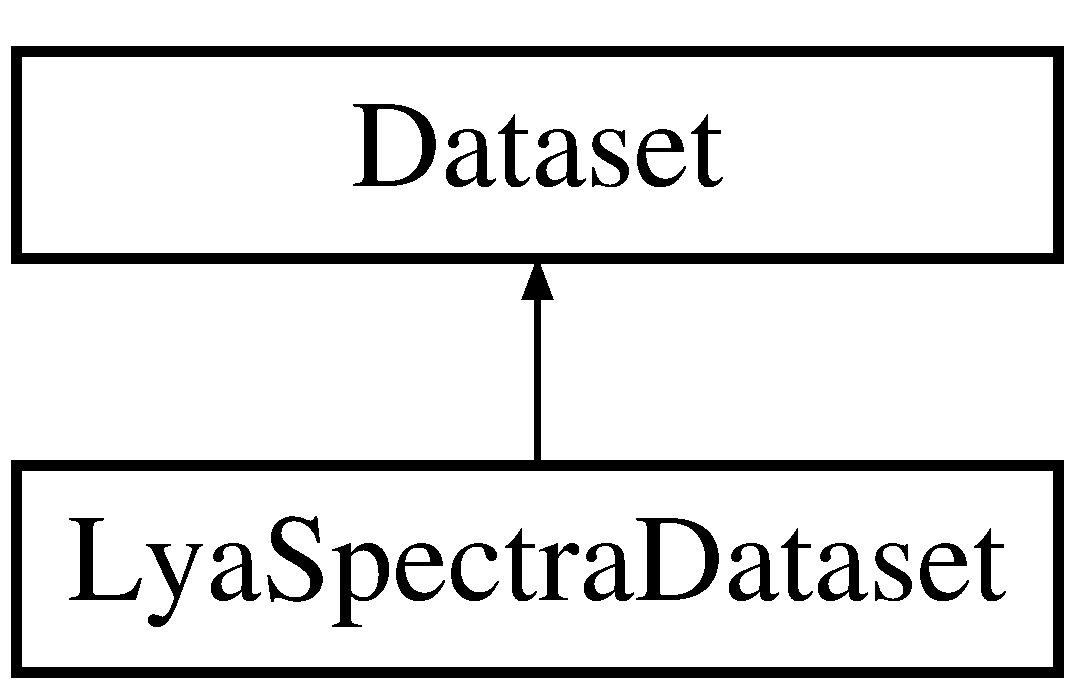
\includegraphics[height=2.000000cm]{class_lya_spectra_dataset}
\end{center}
\end{figure}
\subsection*{Public Member Functions}
\begin{DoxyCompactItemize}
\item 
\hyperlink{class_lya_spectra_dataset_ae9259d54f1bdf5f8b3672a60bbfcd8e6}{Lya\-Spectra\-Dataset} (const \hyperlink{class_global_variables}{Global\-Variables} \&k\-Global\-Variables)
\item 
\hyperlink{struct_plates_map_vector}{Plates\-Map\-Vector}$<$ \hyperlink{class_lya_spectrum}{Lya\-Spectrum} $>$\-::map \hyperlink{class_lya_spectra_dataset_a7b3cef8f52440561301354331230ae95}{list} () const 
\item 
std\-::vector$<$ \hyperlink{class_lya_spectrum}{Lya\-Spectrum} $>$ \hyperlink{class_lya_spectra_dataset_a823b1542931d028564c59fc48da8f7dc}{list} (int plate\-\_\-number) const 
\item 
\hyperlink{class_lya_spectrum}{Lya\-Spectrum} \hyperlink{class_lya_spectra_dataset_a03b47e3cb5016ab62c8916ae1f9f980d}{list} (int plate\-\_\-number, int pos) const 
\item 
int \hyperlink{class_lya_spectra_dataset_a0b10efda4e299ffb8d8ddce45bebfaa9}{Find\-Catalog\-Length} (const std\-::string \&lya\-\_\-spectra\-\_\-catalog)
\item 
void \hyperlink{class_lya_spectra_dataset_a29aa2c3f113d6cbc9d10bfabad12362d}{Give\-R\-A\-D\-E\-C} (std\-::ostream \&out) const 
\item 
void \hyperlink{class_lya_spectra_dataset_a859711c028a33cf935ca5a5a3fb480fd}{Give\-Z} (std\-::ostream \&out) const 
\item 
void \hyperlink{class_lya_spectra_dataset_a85930fd54f392cbfcbea7f49a80b5916}{Load} (const std\-::string \&object\-\_\-list, const std\-::string \&lya\-\_\-spectra\-\_\-dir, const double \&lya\-\_\-wl)
\item 
void \hyperlink{class_lya_spectra_dataset_a444d22db8e799457aef351e74107802e}{Set\-Distances} (const \hyperlink{class_interpolation_map}{Interpolation\-Map} \&redshift\-\_\-distance\-\_\-map)
\end{DoxyCompactItemize}


\subsection{Detailed Description}
\hyperlink{lya__spectra__dataset_8h}{lya\-\_\-spectra\-\_\-dataset.\-h} Purpose\-: This file defines the class \hyperlink{class_lya_spectra_dataset}{Lya\-Spectra\-Dataset}. This class contains the variables necessary to store a spectra dataset. This class is a specialization of the c\-Dataset class

\begin{DoxyAuthor}{Author}
Ignasi Pérez-\/\-Ràfols (\href{mailto:iprafols@icc.ub.edu}{\tt iprafols@icc.\-ub.\-edu}) 
\end{DoxyAuthor}
\begin{DoxyVersion}{Version}
1.\-0 09/17/2014 
\end{DoxyVersion}


Definition at line 35 of file lya\-\_\-spectra\-\_\-dataset.\-h.



\subsection{Constructor \& Destructor Documentation}
\hypertarget{class_lya_spectra_dataset_ae9259d54f1bdf5f8b3672a60bbfcd8e6}{\index{Lya\-Spectra\-Dataset@{Lya\-Spectra\-Dataset}!Lya\-Spectra\-Dataset@{Lya\-Spectra\-Dataset}}
\index{Lya\-Spectra\-Dataset@{Lya\-Spectra\-Dataset}!LyaSpectraDataset@{Lya\-Spectra\-Dataset}}
\subsubsection[{Lya\-Spectra\-Dataset}]{\setlength{\rightskip}{0pt plus 5cm}{\bf Lya\-Spectra\-Dataset\-::\-Lya\-Spectra\-Dataset} (
\begin{DoxyParamCaption}
\item[{const {\bf Global\-Variables} \&}]{k\-Global\-Variables}
\end{DoxyParamCaption}
)}}\label{class_lya_spectra_dataset_ae9259d54f1bdf5f8b3672a60bbfcd8e6}
\hyperlink{lya__spectra__dataset_8cpp}{lya\-\_\-spectra\-\_\-dataset.\-cpp} Purpose\-: This files contains the body for the functions defined in \hyperlink{lya__spectra__dataset_8h}{lya\-\_\-spectra\-\_\-dataset.\-h}

\begin{DoxyAuthor}{Author}
Ignasi Pérez-\/\-Ràfols 
\end{DoxyAuthor}
\begin{DoxyVersion}{Version}
1.\-0 08/08/2014 
\end{DoxyVersion}
E\-X\-P\-L\-A\-N\-A\-T\-I\-O\-N\-: Cosntructs a \hyperlink{class_lya_spectra_dataset}{Lya\-Spectra\-Dataset} instance and loads a catalog of \hyperlink{class_lya_spectrum}{Lya\-Spectrum} objects into it

I\-N\-P\-U\-T\-S\-: k\-Global\-Varialbes -\/ object of type c\-Global\-Variables

O\-U\-T\-P\-U\-T\-S\-: N\-O\-N\-E

C\-L\-A\-S\-S\-E\-S U\-S\-E\-D\-: \hyperlink{class_lya_spectra_dataset}{Lya\-Spectra\-Dataset} \hyperlink{class_global_variables}{Global\-Variables}

F\-U\-N\-C\-I\-T\-O\-N\-S U\-S\-E\-D\-: N\-O\-N\-E

Definition at line 11 of file lya\-\_\-spectra\-\_\-dataset.\-cpp.


\begin{DoxyCode}
                                                                           {
    name_ = kGlobalVariables.lya_spectra_catalog_name();
    Load(kGlobalVariables.lya_spectra_catalog(), kGlobalVariables.
      lya_spectra_dir(), kGlobalVariables.lya_wl());
    
}
\end{DoxyCode}


\subsection{Member Function Documentation}
\hypertarget{class_lya_spectra_dataset_a0b10efda4e299ffb8d8ddce45bebfaa9}{\index{Lya\-Spectra\-Dataset@{Lya\-Spectra\-Dataset}!Find\-Catalog\-Length@{Find\-Catalog\-Length}}
\index{Find\-Catalog\-Length@{Find\-Catalog\-Length}!LyaSpectraDataset@{Lya\-Spectra\-Dataset}}
\subsubsection[{Find\-Catalog\-Length}]{\setlength{\rightskip}{0pt plus 5cm}int {\bf Lya\-Spectra\-Dataset\-::\-Find\-Catalog\-Length} (
\begin{DoxyParamCaption}
\item[{const std\-::string \&}]{lya\-\_\-spectra\-\_\-catalog}
\end{DoxyParamCaption}
)}}\label{class_lya_spectra_dataset_a0b10efda4e299ffb8d8ddce45bebfaa9}
E\-X\-P\-L\-A\-N\-A\-T\-I\-O\-N\-: Finds the number of lines in the provided catalog file list

I\-N\-P\-U\-T\-S\-: lya\-\_\-spectra\-\_\-catalog -\/ name of the list of fits files containing the spectra

O\-U\-T\-P\-U\-T\-S\-: length -\/ an integer containing the number of lines in the catalog file list

C\-L\-A\-S\-S\-E\-S U\-S\-E\-D\-: N\-O\-N\-E

F\-U\-N\-C\-I\-T\-O\-N\-S U\-S\-E\-D\-: N\-O\-N\-E

Definition at line 35 of file lya\-\_\-spectra\-\_\-dataset.\-cpp.


\begin{DoxyCode}
                                                                            {
    std::string cmd = "wc -l "+lya_spectra_catalog;
    char path[PATH_MAX];
    FILE* pipe = popen(cmd.c_str(),"r");
    
    fgets(path, PATH_MAX, pipe);
    
    int length = atoi(strtok(path," "));

    return length;
}
\end{DoxyCode}
\hypertarget{class_lya_spectra_dataset_a29aa2c3f113d6cbc9d10bfabad12362d}{\index{Lya\-Spectra\-Dataset@{Lya\-Spectra\-Dataset}!Give\-R\-A\-D\-E\-C@{Give\-R\-A\-D\-E\-C}}
\index{Give\-R\-A\-D\-E\-C@{Give\-R\-A\-D\-E\-C}!LyaSpectraDataset@{Lya\-Spectra\-Dataset}}
\subsubsection[{Give\-R\-A\-D\-E\-C}]{\setlength{\rightskip}{0pt plus 5cm}void {\bf Lya\-Spectra\-Dataset\-::\-Give\-R\-A\-D\-E\-C} (
\begin{DoxyParamCaption}
\item[{std\-::ostream \&}]{out}
\end{DoxyParamCaption}
) const\hspace{0.3cm}{\ttfamily  \mbox{[}virtual\mbox{]}}}}\label{class_lya_spectra_dataset_a29aa2c3f113d6cbc9d10bfabad12362d}
E\-X\-P\-L\-A\-N\-A\-T\-I\-O\-N\-: Adds the objects' R\-A-\/\-D\-E\-C values to out

I\-N\-P\-U\-T\-S\-: out -\/ an ostream to add the objects' R\-A-\/\-D\-E\-C values to

O\-U\-T\-P\-U\-T\-S\-: N\-O\-N\-E

C\-L\-A\-S\-S\-E\-S U\-S\-E\-D\-: \hyperlink{class_lya_spectrum}{Lya\-Spectrum} \hyperlink{class_lya_spectra_dataset}{Lya\-Spectra\-Dataset}

F\-U\-N\-C\-I\-T\-O\-N\-S U\-S\-E\-D\-: N\-O\-N\-E

Implements \hyperlink{class_dataset_a5867a14c1554b50ce062bdacd36460af}{Dataset}.



Definition at line 64 of file lya\-\_\-spectra\-\_\-dataset.\-cpp.


\begin{DoxyCode}
                                                      {
    for (PlatesMapVector<LyaSpectrum>::map::const_iterator it = list_.begin(); 
      it != list_.end(); it ++){
        for (size_t i = 0; i < (*it).second.size(); i ++){
            out << (*it).second[i].angle() << std::endl;
        }
    }
    
}
\end{DoxyCode}
\hypertarget{class_lya_spectra_dataset_a859711c028a33cf935ca5a5a3fb480fd}{\index{Lya\-Spectra\-Dataset@{Lya\-Spectra\-Dataset}!Give\-Z@{Give\-Z}}
\index{Give\-Z@{Give\-Z}!LyaSpectraDataset@{Lya\-Spectra\-Dataset}}
\subsubsection[{Give\-Z}]{\setlength{\rightskip}{0pt plus 5cm}void {\bf Lya\-Spectra\-Dataset\-::\-Give\-Z} (
\begin{DoxyParamCaption}
\item[{std\-::ostream \&}]{out}
\end{DoxyParamCaption}
) const\hspace{0.3cm}{\ttfamily  \mbox{[}virtual\mbox{]}}}}\label{class_lya_spectra_dataset_a859711c028a33cf935ca5a5a3fb480fd}
E\-X\-P\-L\-A\-N\-A\-T\-I\-O\-N\-: Adds the objects' redshift values to out

I\-N\-P\-U\-T\-S\-: out -\/ an ostream to add the objects' redshift values to

O\-U\-T\-P\-U\-T\-S\-: N\-O\-N\-E

C\-L\-A\-S\-S\-E\-S U\-S\-E\-D\-: \hyperlink{class_lya_pixel}{Lya\-Pixel} \hyperlink{class_lya_spectrum}{Lya\-Spectrum} \hyperlink{class_lya_spectra_dataset}{Lya\-Spectra\-Dataset}

F\-U\-N\-C\-I\-T\-O\-N\-S U\-S\-E\-D\-: N\-O\-N\-E

Implements \hyperlink{class_dataset_aae82d78ec374da243c22a96236b39465}{Dataset}.



Definition at line 91 of file lya\-\_\-spectra\-\_\-dataset.\-cpp.


\begin{DoxyCode}
                                                  {
    for (PlatesMapVector<LyaSpectrum>::map::const_iterator it = list_.begin(); 
      it != list_.end(); it ++){
        for (size_t i = 0; i < (*it).second.size(); i ++){
            for (size_t j = 0; j < (*it).second[i].SpectrumSize(); j++){
                out << (*it).second[i].spectrum(j).z() << std::endl;
            }
        }
    }
    
}
\end{DoxyCode}
\hypertarget{class_lya_spectra_dataset_a7b3cef8f52440561301354331230ae95}{\index{Lya\-Spectra\-Dataset@{Lya\-Spectra\-Dataset}!list@{list}}
\index{list@{list}!LyaSpectraDataset@{Lya\-Spectra\-Dataset}}
\subsubsection[{list}]{\setlength{\rightskip}{0pt plus 5cm}{\bf Plates\-Map\-Vector}$<${\bf Lya\-Spectrum}$>$\-::map {\bf Lya\-Spectra\-Dataset\-::list} (
\begin{DoxyParamCaption}
{}
\end{DoxyParamCaption}
) const\hspace{0.3cm}{\ttfamily  \mbox{[}inline\mbox{]}}}}\label{class_lya_spectra_dataset_a7b3cef8f52440561301354331230ae95}


Definition at line 48 of file lya\-\_\-spectra\-\_\-dataset.\-h.


\begin{DoxyCode}
{return list_;}
\end{DoxyCode}
\hypertarget{class_lya_spectra_dataset_a823b1542931d028564c59fc48da8f7dc}{\index{Lya\-Spectra\-Dataset@{Lya\-Spectra\-Dataset}!list@{list}}
\index{list@{list}!LyaSpectraDataset@{Lya\-Spectra\-Dataset}}
\subsubsection[{list}]{\setlength{\rightskip}{0pt plus 5cm}std\-::vector$<${\bf Lya\-Spectrum}$>$ {\bf Lya\-Spectra\-Dataset\-::list} (
\begin{DoxyParamCaption}
\item[{int}]{plate\-\_\-number}
\end{DoxyParamCaption}
) const\hspace{0.3cm}{\ttfamily  \mbox{[}inline\mbox{]}}}}\label{class_lya_spectra_dataset_a823b1542931d028564c59fc48da8f7dc}


Definition at line 49 of file lya\-\_\-spectra\-\_\-dataset.\-h.


\begin{DoxyCode}
{return (*list_.find(plate_number)).second;}
\end{DoxyCode}
\hypertarget{class_lya_spectra_dataset_a03b47e3cb5016ab62c8916ae1f9f980d}{\index{Lya\-Spectra\-Dataset@{Lya\-Spectra\-Dataset}!list@{list}}
\index{list@{list}!LyaSpectraDataset@{Lya\-Spectra\-Dataset}}
\subsubsection[{list}]{\setlength{\rightskip}{0pt plus 5cm}{\bf Lya\-Spectrum} {\bf Lya\-Spectra\-Dataset\-::list} (
\begin{DoxyParamCaption}
\item[{int}]{plate\-\_\-number, }
\item[{int}]{pos}
\end{DoxyParamCaption}
) const\hspace{0.3cm}{\ttfamily  \mbox{[}inline\mbox{]}}}}\label{class_lya_spectra_dataset_a03b47e3cb5016ab62c8916ae1f9f980d}


Definition at line 50 of file lya\-\_\-spectra\-\_\-dataset.\-h.


\begin{DoxyCode}
{return (*list_.find(plate_number)).second[pos];}
\end{DoxyCode}
\hypertarget{class_lya_spectra_dataset_a85930fd54f392cbfcbea7f49a80b5916}{\index{Lya\-Spectra\-Dataset@{Lya\-Spectra\-Dataset}!Load@{Load}}
\index{Load@{Load}!LyaSpectraDataset@{Lya\-Spectra\-Dataset}}
\subsubsection[{Load}]{\setlength{\rightskip}{0pt plus 5cm}void {\bf Lya\-Spectra\-Dataset\-::\-Load} (
\begin{DoxyParamCaption}
\item[{const std\-::string \&}]{object\-\_\-list, }
\item[{const std\-::string \&}]{lya\-\_\-spectra\-\_\-dir, }
\item[{const double \&}]{lya\-\_\-wl}
\end{DoxyParamCaption}
)}}\label{class_lya_spectra_dataset_a85930fd54f392cbfcbea7f49a80b5916}
E\-X\-P\-L\-A\-N\-A\-T\-I\-O\-N\-: Loads the object dataset from a catalog file

I\-N\-P\-U\-T\-S\-: lya\-\_\-spectra\-\_\-catalog -\/ a string with the name of the list of fits files containing the spectra lya\-\_\-spectra\-\_\-dir -\/ a string with the directory where the ly-\/a spectrum files are stored lya\-\_\-wl -\/ a double with the wavelength of the lyman-\/alpha line (in Angstroms)

O\-U\-T\-P\-U\-T\-S\-: N\-O\-N\-E

C\-L\-A\-S\-S\-E\-S U\-S\-E\-D\-: \hyperlink{class_lya_spectrum}{Lya\-Spectrum} \hyperlink{class_lya_spectra_dataset}{Lya\-Spectra\-Dataset}

F\-U\-N\-C\-I\-T\-O\-N\-S U\-S\-E\-D\-: N\-O\-N\-E

Definition at line 121 of file lya\-\_\-spectra\-\_\-dataset.\-cpp.


\begin{DoxyCode}
                                                                               
                                               {
    // resizing astro_object_pointer
    size_ = FindCatalogLength(lya_spectra_catalog);

    // open catalog
    std::ifstream catalog(lya_spectra_catalog.c_str());
    if (catalog.is_open()){
        std::string file("");        
        while (getline(catalog,file)){
            
            // create LyaSpectrum
            LyaSpectrum object(lya_spectra_dir + file, lya_wl);
            
            // adding object to list_
            if (list_.find(object.plate()) == list_.end()){
                // if necessary, create new entry
                std::vector<LyaSpectrum> v;
                list_[object.plate()] = v;
                num_objects_in_plate_[object.plate()] = 0;
            }
            (*list_.find(object.plate())).second.push_back(object);
            
            // updating number_of_objects_in_plate
            (*num_objects_in_plate_.find(object.plate())).second ++;
        }
    }
    else{
        std::cout << "Error: could not read spectra catalog" << std::endl;
    }
}
\end{DoxyCode}
\hypertarget{class_lya_spectra_dataset_a444d22db8e799457aef351e74107802e}{\index{Lya\-Spectra\-Dataset@{Lya\-Spectra\-Dataset}!Set\-Distances@{Set\-Distances}}
\index{Set\-Distances@{Set\-Distances}!LyaSpectraDataset@{Lya\-Spectra\-Dataset}}
\subsubsection[{Set\-Distances}]{\setlength{\rightskip}{0pt plus 5cm}void {\bf Lya\-Spectra\-Dataset\-::\-Set\-Distances} (
\begin{DoxyParamCaption}
\item[{const {\bf Interpolation\-Map} \&}]{redshift\-\_\-distance\-\_\-map}
\end{DoxyParamCaption}
)\hspace{0.3cm}{\ttfamily  \mbox{[}virtual\mbox{]}}}}\label{class_lya_spectra_dataset_a444d22db8e799457aef351e74107802e}
E\-X\-P\-L\-A\-N\-A\-T\-I\-O\-N\-: Sets the distance to every object in the dataset

I\-N\-P\-U\-T\-S\-: redshif\-\_\-distance\-\_\-map -\/ a \hyperlink{class_interpolation_map}{Interpolation\-Map} instance with the redshift-\/distance relation

O\-U\-T\-P\-U\-T\-S\-: N\-O\-N\-E

C\-L\-A\-S\-S\-E\-S U\-S\-E\-D\-: \hyperlink{class_lya_spectrum}{Lya\-Spectrum} \hyperlink{class_lya_spectra_dataset}{Lya\-Spectra\-Dataset} \hyperlink{class_interpolation_map}{Interpolation\-Map}

F\-U\-N\-C\-I\-T\-O\-N\-S U\-S\-E\-D\-: N\-O\-N\-E

Implements \hyperlink{class_dataset_a76dbae8574850da55a3b88149ccbe3f9}{Dataset}.



Definition at line 172 of file lya\-\_\-spectra\-\_\-dataset.\-cpp.


\begin{DoxyCode}
                                                                               
        {
    for (PlatesMapVector<LyaSpectrum>::map::iterator it = list_.begin(); it != 
      list_.end(); it ++){
        for (size_t i = 0; i < (*it).second.size(); i ++){
            (*it).second[i].SetDistance(redshift_distance_map);
        }
    }
    
}
\end{DoxyCode}


The documentation for this class was generated from the following files\-:\begin{DoxyCompactItemize}
\item 
\hyperlink{lya__spectra__dataset_8h}{lya\-\_\-spectra\-\_\-dataset.\-h}\item 
\hyperlink{lya__spectra__dataset_8cpp}{lya\-\_\-spectra\-\_\-dataset.\-cpp}\end{DoxyCompactItemize}

\hypertarget{class_lya_spectrum}{\section{Lya\-Spectrum Class Reference}
\label{class_lya_spectrum}\index{Lya\-Spectrum@{Lya\-Spectrum}}
}


{\ttfamily \#include $<$lya\-\_\-spectrum.\-h$>$}

Inheritance diagram for Lya\-Spectrum\-:\begin{figure}[H]
\begin{center}
\leavevmode
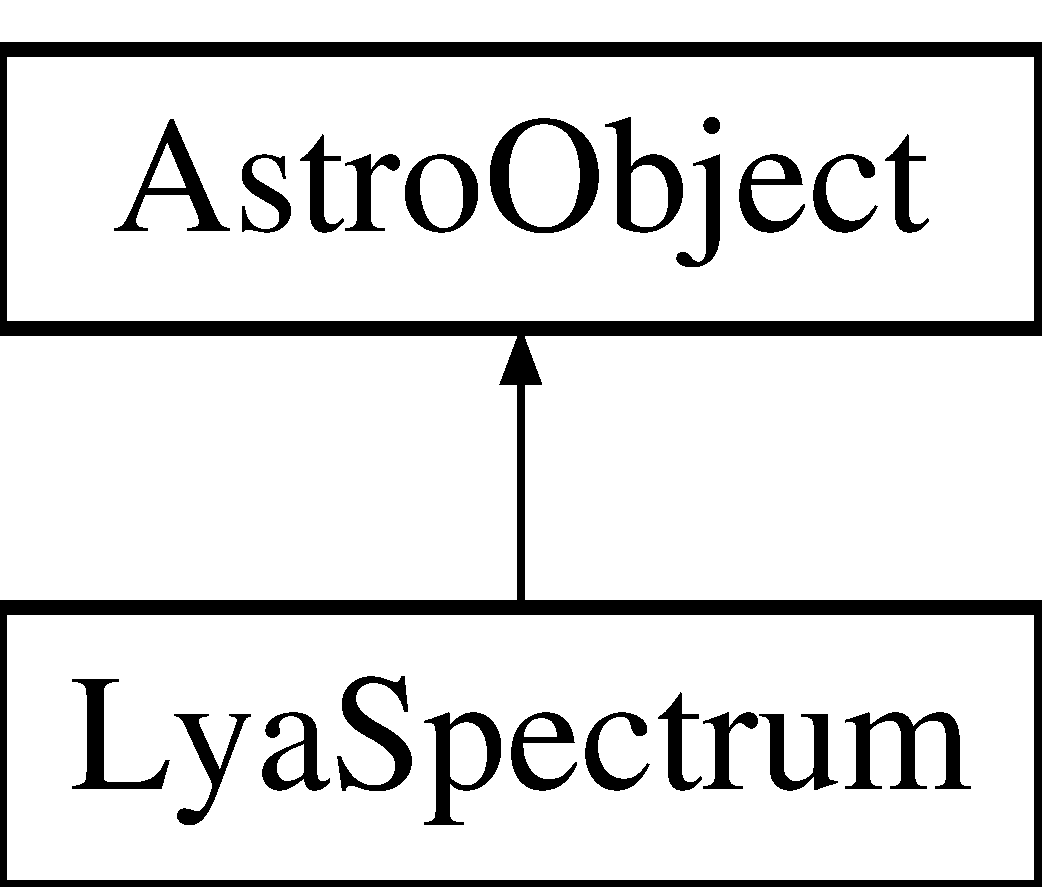
\includegraphics[height=2.000000cm]{class_lya_spectrum}
\end{center}
\end{figure}
\subsection*{Public Member Functions}
\begin{DoxyCompactItemize}
\item 
\hyperlink{class_lya_spectrum_a28194690040c52a02f196ea47cad4adc}{Lya\-Spectrum} (const std\-::string \&filename, const double \&lya\-\_\-wl, const bool radians=true)
\item 
std\-::vector$<$ \hyperlink{class_lya_pixel}{Lya\-Pixel} $>$ \hyperlink{class_lya_spectrum_ab3532ecc27237cbb5231f386e1b94a62}{spectrum} () const 
\item 
\hyperlink{class_lya_pixel}{Lya\-Pixel} \hyperlink{class_lya_spectrum_a371b8e381330aded034d8c6bfb4743df}{spectrum} (size\-\_\-t i) const 
\item 
void \hyperlink{class_lya_spectrum_a5aed91d841c38e3c399e2b84b05fd2d3}{Set\-Distance} (const \hyperlink{class_interpolation_map}{Interpolation\-Map} \&redshift\-\_\-distance\-\_\-map)
\item 
size\-\_\-t \hyperlink{class_lya_spectrum_aff44677f212bf5a327d899ccbc86a5d9}{Spectrum\-Size} () const 
\end{DoxyCompactItemize}


\subsection{Detailed Description}
\hyperlink{lya__spectrum_8h}{lya\-\_\-spectrum.\-h} Purpose\-: This file defines the class \hyperlink{class_lya_spectrum}{Lya\-Spectrum}. This class contains the variables necessary to store a lyman-\/alpha spectrum. This class is a specialization of the c\-Astro\-Object class

\begin{DoxyAuthor}{Author}
Ignasi Pérez-\/\-Ràfols (\href{mailto:iprafols@icc.ub.edu}{\tt iprafols@icc.\-ub.\-edu}) 
\end{DoxyAuthor}
\begin{DoxyVersion}{Version}
1.\-0 09/18/2014 
\end{DoxyVersion}


Definition at line 35 of file lya\-\_\-spectrum.\-h.



\subsection{Constructor \& Destructor Documentation}
\hypertarget{class_lya_spectrum_a28194690040c52a02f196ea47cad4adc}{\index{Lya\-Spectrum@{Lya\-Spectrum}!Lya\-Spectrum@{Lya\-Spectrum}}
\index{Lya\-Spectrum@{Lya\-Spectrum}!LyaSpectrum@{Lya\-Spectrum}}
\subsubsection[{Lya\-Spectrum}]{\setlength{\rightskip}{0pt plus 5cm}{\bf Lya\-Spectrum\-::\-Lya\-Spectrum} (
\begin{DoxyParamCaption}
\item[{const std\-::string \&}]{filename, }
\item[{const double \&}]{lya\-\_\-wl, }
\item[{const bool}]{radians = {\ttfamily true}}
\end{DoxyParamCaption}
)}}\label{class_lya_spectrum_a28194690040c52a02f196ea47cad4adc}
\hyperlink{lya__spectrum_8cpp}{lya\-\_\-spectrum.\-cpp} Purpose\-: This files contains the body for the functions defined in \hyperlink{lya__spectrum_8h}{lya\-\_\-spectrum.\-h}

\begin{DoxyAuthor}{Author}
Ignasi Pérez-\/\-Ràfols 
\end{DoxyAuthor}
\begin{DoxyVersion}{Version}
1.\-0 09/18/2014 
\end{DoxyVersion}
E\-X\-P\-L\-A\-N\-A\-T\-I\-O\-N\-: Cosntructs a \hyperlink{class_lya_spectrum}{Lya\-Spectrum} instance

I\-N\-P\-U\-T\-S\-: filename -\/ a string containing the spectrum's fits file name

O\-U\-T\-P\-U\-T\-S\-: N\-O\-N\-E

C\-L\-A\-S\-S\-E\-S U\-S\-E\-D\-: \hyperlink{class_lya_spectrum}{Lya\-Spectrum} \hyperlink{class_lya_pixel}{Lya\-Pixel} \hyperlink{class_sphere_point}{Sphere\-Point}

F\-U\-N\-C\-I\-T\-O\-N\-S U\-S\-E\-D\-: N\-O\-N\-E

Definition at line 11 of file lya\-\_\-spectrum.\-cpp.


\begin{DoxyCode}
                                                                               
                  {
    // setting the catalog columns to be read
    std::vector<std::string> fields(3);
    fields[0] = "LOGLAM";
    fields[1] = "FOREST";
    fields[2] = "WEIGHT";
    

    // construct fits object
    std::auto_ptr<CCfits::FITS> pInfile; 
    
    try{
        
        pInfile = std::auto_ptr<CCfits::FITS>(new CCfits::FITS(filename,
      CCfits::Read,1,true,fields));
        
    } catch(CCfits::FITS::CantOpen x) {
        
        throw "Error occured in cAstroObjectDataset constructor: couldn't open
       catalog file: " + filename;
    }
    CCfits::ExtHDU& data = pInfile->extension(1);
    
    // number of lines in the file
    long NAXIS2 = data.axis(1);
    size_t nobj = NAXIS2;
    spectrum_.reserve(nobj);
    
    // this will store the information
    std::valarray<double> loglam, forest, weight;
    
    // reading data
    data.column(fields[0]).read(loglam, 1, nobj); // logarithm of the
       wavelength value
    data.column(fields[1]).read(forest, 1, nobj); // normalized flux in the
       ly-alpha forest
    data.column(fields[2]).read(weight, 1, nobj); // weight
    
    for (int i=0;i<nobj;i++){
        // create LyaPixel
        LyaPixel object(loglam[i], lya_wl, forest[i], weight[i]);
            
        // adding object to spectrum_
        spectrum_.push_back(object);
    }
    
    // reading header
    data.readAllKeys();
    
    // extract right ascension
    std::string sra("RA");
    double ra;
    data.keyWord(sra).value(ra);
     
    // extract declination
    std::string sdec("DEC");
    double dec;
    data.keyWord(sdec).value(dec);
     
    // set angular position
    if (not radians){
        ra *= acos(-1)/180.0;
        dec *= acos(-1)/180.0;
    }
    SpherePoint angle(ra, dec);
    angle_ = angle;
    
    // extract redshift
    std::string sz("Z");
    data.keyWord(sdec).value(z_);
    
    // extract plate, mjd and fiber numbers
    std::string spmf("PMF");
    std::string pmf;
    data.keyWord(spmf).value(pmf);
    
    plate_ = atoi(strtok((char*)pmf.c_str(),"-"));
    mjd_ = atoi(strtok((char*)pmf.c_str(),"-"));
    fiber_ = atoi(strtok((char*)pmf.c_str(),"-"));

}
\end{DoxyCode}


\subsection{Member Function Documentation}
\hypertarget{class_lya_spectrum_a5aed91d841c38e3c399e2b84b05fd2d3}{\index{Lya\-Spectrum@{Lya\-Spectrum}!Set\-Distance@{Set\-Distance}}
\index{Set\-Distance@{Set\-Distance}!LyaSpectrum@{Lya\-Spectrum}}
\subsubsection[{Set\-Distance}]{\setlength{\rightskip}{0pt plus 5cm}void {\bf Lya\-Spectrum\-::\-Set\-Distance} (
\begin{DoxyParamCaption}
\item[{const {\bf Interpolation\-Map} \&}]{redshift\-\_\-distance\-\_\-map}
\end{DoxyParamCaption}
)\hspace{0.3cm}{\ttfamily  \mbox{[}virtual\mbox{]}}}}\label{class_lya_spectrum_a5aed91d841c38e3c399e2b84b05fd2d3}
E\-X\-P\-L\-A\-N\-A\-T\-I\-O\-N\-: Sets the distance to object

I\-N\-P\-U\-T\-S\-: redshif\-\_\-distance\-\_\-map -\/ a \hyperlink{class_interpolation_map}{Interpolation\-Map} instance with the redshift-\/distance relation

O\-U\-T\-P\-U\-T\-S\-: N\-O\-N\-E

C\-L\-A\-S\-S\-E\-S U\-S\-E\-D\-: \hyperlink{class_astro_object}{Astro\-Object}

F\-U\-N\-C\-I\-T\-O\-N\-S U\-S\-E\-D\-: N\-O\-N\-E

Reimplemented from \hyperlink{class_astro_object_a7addd0f108191b1ca35db6e16e45ed72}{Astro\-Object}.



Definition at line 108 of file lya\-\_\-spectrum.\-cpp.


\begin{DoxyCode}
                                                                          {
    dist_ = NAN;
    
    for (size_t i = 0; i < spectrum_.size(); i++){
        spectrum_[i].SetDistance(redshift_distance_map);
    }
    
}\end{DoxyCode}
\hypertarget{class_lya_spectrum_ab3532ecc27237cbb5231f386e1b94a62}{\index{Lya\-Spectrum@{Lya\-Spectrum}!spectrum@{spectrum}}
\index{spectrum@{spectrum}!LyaSpectrum@{Lya\-Spectrum}}
\subsubsection[{spectrum}]{\setlength{\rightskip}{0pt plus 5cm}std\-::vector$<${\bf Lya\-Pixel}$>$ {\bf Lya\-Spectrum\-::spectrum} (
\begin{DoxyParamCaption}
{}
\end{DoxyParamCaption}
) const\hspace{0.3cm}{\ttfamily  \mbox{[}inline\mbox{]}}}}\label{class_lya_spectrum_ab3532ecc27237cbb5231f386e1b94a62}


Definition at line 48 of file lya\-\_\-spectrum.\-h.


\begin{DoxyCode}
{return spectrum_;}
\end{DoxyCode}
\hypertarget{class_lya_spectrum_a371b8e381330aded034d8c6bfb4743df}{\index{Lya\-Spectrum@{Lya\-Spectrum}!spectrum@{spectrum}}
\index{spectrum@{spectrum}!LyaSpectrum@{Lya\-Spectrum}}
\subsubsection[{spectrum}]{\setlength{\rightskip}{0pt plus 5cm}{\bf Lya\-Pixel} {\bf Lya\-Spectrum\-::spectrum} (
\begin{DoxyParamCaption}
\item[{size\-\_\-t}]{i}
\end{DoxyParamCaption}
) const\hspace{0.3cm}{\ttfamily  \mbox{[}inline\mbox{]}}}}\label{class_lya_spectrum_a371b8e381330aded034d8c6bfb4743df}


Definition at line 49 of file lya\-\_\-spectrum.\-h.


\begin{DoxyCode}
{return spectrum_[i];}
\end{DoxyCode}
\hypertarget{class_lya_spectrum_aff44677f212bf5a327d899ccbc86a5d9}{\index{Lya\-Spectrum@{Lya\-Spectrum}!Spectrum\-Size@{Spectrum\-Size}}
\index{Spectrum\-Size@{Spectrum\-Size}!LyaSpectrum@{Lya\-Spectrum}}
\subsubsection[{Spectrum\-Size}]{\setlength{\rightskip}{0pt plus 5cm}size\-\_\-t {\bf Lya\-Spectrum\-::\-Spectrum\-Size} (
\begin{DoxyParamCaption}
{}
\end{DoxyParamCaption}
) const\hspace{0.3cm}{\ttfamily  \mbox{[}inline\mbox{]}}}}\label{class_lya_spectrum_aff44677f212bf5a327d899ccbc86a5d9}


Definition at line 58 of file lya\-\_\-spectrum.\-h.


\begin{DoxyCode}
{return spectrum_.size();}
\end{DoxyCode}


The documentation for this class was generated from the following files\-:\begin{DoxyCompactItemize}
\item 
\hyperlink{lya__spectrum_8h}{lya\-\_\-spectrum.\-h}\item 
\hyperlink{lya__spectrum_8cpp}{lya\-\_\-spectrum.\-cpp}\end{DoxyCompactItemize}

\hypertarget{class_plate}{\section{Plate Class Reference}
\label{class_plate}\index{Plate@{Plate}}
}


{\ttfamily \#include $<$plate.\-h$>$}

Inheritance diagram for Plate\-:\begin{figure}[H]
\begin{center}
\leavevmode
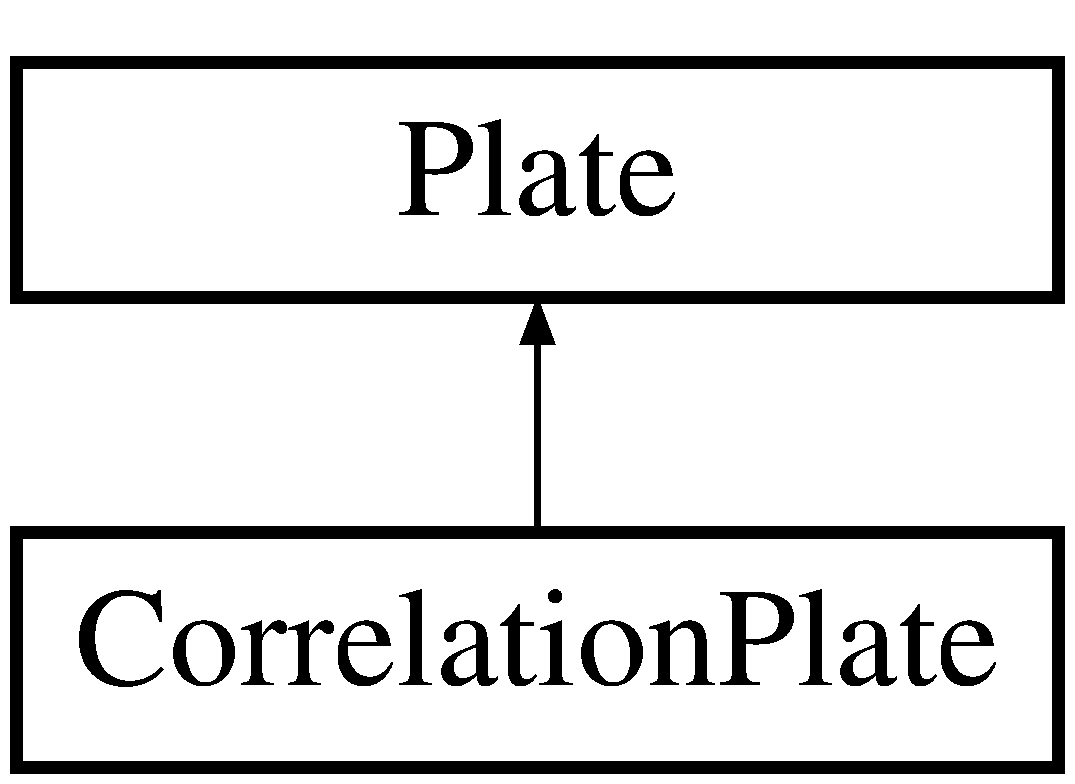
\includegraphics[height=2.000000cm]{class_plate}
\end{center}
\end{figure}
\subsection*{Public Member Functions}
\begin{DoxyCompactItemize}
\item 
\hyperlink{class_plate_aaa77995d1d6acb3f0a9437b8685d5294}{Plate} ()
\item 
\hyperlink{class_plate_a898513f63d991c44add2f1b3e0d771d7}{Plate} (const std\-::string \&filename)
\item 
\hyperlink{class_sphere_point}{Sphere\-Point} \hyperlink{class_plate_a3ca2ca2397d5754d7f599e828d6428ae}{angle} () const 
\item 
double \hyperlink{class_plate_ab350a5bd0d3334e435b2bd52b125cc6e}{number\-\_\-of\-\_\-objects} () const 
\item 
int \hyperlink{class_plate_a74d31939a29286c82ecd8fc7daf075ed}{plate\-\_\-number} () const 
\item 
void \hyperlink{class_plate_a369d3b556e0cb3a7e5bb0cdb9fab6766}{set\-\_\-plate\-\_\-number} (int number)
\item 
bool \hyperlink{class_plate_a1c5e1122f86590fa18551e4874df9603}{Is\-Neighbour} (const \hyperlink{class_plate}{Plate} \&plate, const double \&neighbours\-\_\-max\-\_\-distance)
\item 
void \hyperlink{class_plate_af8c7b2cbadfd5359e7464f6015cbf21c}{Normalize} ()
\item 
void \hyperlink{class_plate_ab7b0d84a37d69bb228331d2f0b482c34}{Update\-R\-A\-D\-E\-C\-Values} (const \hyperlink{class_plate}{Plate} \&plate)
\end{DoxyCompactItemize}
\subsection*{Protected Attributes}
\begin{DoxyCompactItemize}
\item 
int \hyperlink{class_plate_a3ff23f95b9f615a470a315cadc2b8940}{plate\-\_\-number\-\_\-}
\end{DoxyCompactItemize}


\subsection{Detailed Description}
\hyperlink{plate_8h}{plate.\-h} Purpose\-: This file defines the class \hyperlink{class_plate}{Plate}. This class contains number of the plate and its mean values of right ascension and declination

\begin{DoxyAuthor}{Author}
Ignasi Pérez-\/\-Ràfols (\href{mailto:iprafols@icc.ub.edu}{\tt iprafols@icc.\-ub.\-edu}) 
\end{DoxyAuthor}
\begin{DoxyVersion}{Version}
1.\-0 06/26/2014 
\end{DoxyVersion}


Definition at line 30 of file plate.\-h.



\subsection{Constructor \& Destructor Documentation}
\hypertarget{class_plate_aaa77995d1d6acb3f0a9437b8685d5294}{\index{Plate@{Plate}!Plate@{Plate}}
\index{Plate@{Plate}!Plate@{Plate}}
\subsubsection[{Plate}]{\setlength{\rightskip}{0pt plus 5cm}{\bf Plate\-::\-Plate} (
\begin{DoxyParamCaption}
{}
\end{DoxyParamCaption}
)\hspace{0.3cm}{\ttfamily  \mbox{[}inline\mbox{]}}}}\label{class_plate_aaa77995d1d6acb3f0a9437b8685d5294}


Definition at line 37 of file plate.\-h.


\begin{DoxyCode}
{};
\end{DoxyCode}
\hypertarget{class_plate_a898513f63d991c44add2f1b3e0d771d7}{\index{Plate@{Plate}!Plate@{Plate}}
\index{Plate@{Plate}!Plate@{Plate}}
\subsubsection[{Plate}]{\setlength{\rightskip}{0pt plus 5cm}{\bf Plate\-::\-Plate} (
\begin{DoxyParamCaption}
\item[{const std\-::string \&}]{filename}
\end{DoxyParamCaption}
)}}\label{class_plate_a898513f63d991c44add2f1b3e0d771d7}
\hyperlink{plate_8cpp}{plate.\-cpp} Purpose\-: This files contains the body for the functions defined in \hyperlink{plate_8h}{plate.\-h}

\begin{DoxyAuthor}{Author}
Ignasi Pérez-\/\-Ràfols 
\end{DoxyAuthor}
\begin{DoxyVersion}{Version}
1.\-0 06/26/2014 
\end{DoxyVersion}
E\-X\-P\-L\-A\-N\-A\-T\-I\-O\-N\-: Cosntructs a \hyperlink{class_plate}{Plate} instance and initializes all its variables

I\-N\-P\-U\-T\-S\-: filename -\/ string containing the full path of the fits file containing the object

O\-U\-T\-P\-U\-T\-S\-: N\-O\-N\-E

C\-L\-A\-S\-S\-E\-S U\-S\-E\-D\-: \hyperlink{class_plate}{Plate}

F\-U\-N\-C\-I\-T\-O\-N\-S U\-S\-E\-D\-: N\-O\-N\-E

Definition at line 11 of file plate.\-cpp.


\begin{DoxyCode}
                                     {
    // constructs fits object
    std::auto_ptr<CCfits::FITS> pInfile;//std::unique_ptr<FITS> pInfile;
    
    try{
        
        pInfile = std::auto_ptr<CCfits::FITS>(new CCfits::FITS(filename, 
      CCfits::Read));//std::unique_ptr<FITS>(new FITS(filename, Read));
        
    } catch(CCfits::FITS::CantOpen x) {
        
        throw "cPlate::cPlate(" + filename + ") failed";
    }

    // define a reference for clarity
    CCfits::ExtHDU& data = (*pInfile).extension(1);
    
    // reading header
    data.readAllKeys();
    
    // extract right ascension
    std::string sra("RA");
    double ra;
    data.keyWord(sra).value(ra);
    
    // extract declination
    std::string sdec("DEC");
    double dec;
    data.keyWord(sdec).value(dec);
    
    // extract plate number
    std::string spmf("PMF");
    std::string pmf;
    data.keyWord(spmf).value(pmf);
    
    // set plate number
    plate_number_ = atoi(strtok((char*)pmf.c_str(),"-"));
    
    // set number of averaged objects to 1
    number_of_objects_ = 1.0;
    
    // set position angle
    SpherePoint angle(ra, dec);
    angle_ = angle;
}
\end{DoxyCode}


\subsection{Member Function Documentation}
\hypertarget{class_plate_a3ca2ca2397d5754d7f599e828d6428ae}{\index{Plate@{Plate}!angle@{angle}}
\index{angle@{angle}!Plate@{Plate}}
\subsubsection[{angle}]{\setlength{\rightskip}{0pt plus 5cm}{\bf Sphere\-Point} {\bf Plate\-::angle} (
\begin{DoxyParamCaption}
{}
\end{DoxyParamCaption}
) const\hspace{0.3cm}{\ttfamily  \mbox{[}inline\mbox{]}}}}\label{class_plate_a3ca2ca2397d5754d7f599e828d6428ae}


Definition at line 45 of file plate.\-h.


\begin{DoxyCode}
{return angle_;}
\end{DoxyCode}
\hypertarget{class_plate_a1c5e1122f86590fa18551e4874df9603}{\index{Plate@{Plate}!Is\-Neighbour@{Is\-Neighbour}}
\index{Is\-Neighbour@{Is\-Neighbour}!Plate@{Plate}}
\subsubsection[{Is\-Neighbour}]{\setlength{\rightskip}{0pt plus 5cm}bool {\bf Plate\-::\-Is\-Neighbour} (
\begin{DoxyParamCaption}
\item[{const {\bf Plate} \&}]{plate, }
\item[{const double \&}]{neighbours\-\_\-max\-\_\-distance}
\end{DoxyParamCaption}
)}}\label{class_plate_a1c5e1122f86590fa18551e4874df9603}
E\-X\-P\-L\-A\-N\-A\-T\-I\-O\-N\-: Returns true if the given plate is a neighbour plate and false otherwise

I\-N\-P\-U\-T\-S\-: plate -\/ plate to check neighbourhood with dist -\/ maximum angular separation for a couple of plates to be considered neighbours (in radians)

O\-U\-T\-P\-U\-T\-S\-: N\-O\-N\-E

C\-L\-A\-S\-S\-E\-S U\-S\-E\-D\-: \hyperlink{class_plate}{Plate}

F\-U\-N\-C\-I\-T\-O\-N\-S U\-S\-E\-D\-: N\-O\-N\-E

Definition at line 73 of file plate.\-cpp.


\begin{DoxyCode}
                                                                               
      {
    return angle_.AngularDistance(plate.angle()) <= neighbours_max_distance;
}
\end{DoxyCode}
\hypertarget{class_plate_af8c7b2cbadfd5359e7464f6015cbf21c}{\index{Plate@{Plate}!Normalize@{Normalize}}
\index{Normalize@{Normalize}!Plate@{Plate}}
\subsubsection[{Normalize}]{\setlength{\rightskip}{0pt plus 5cm}void {\bf Plate\-::\-Normalize} (
\begin{DoxyParamCaption}
{}
\end{DoxyParamCaption}
)}}\label{class_plate_af8c7b2cbadfd5359e7464f6015cbf21c}
E\-X\-P\-L\-A\-N\-A\-T\-I\-O\-N\-: Normalizes angle\-\_\- by dividing it by number\-\_\-of\-\_\-objects\-\_\-. Then it sets number\-\_\-of\-\_\-objects\-\_\- to 0 and updates sin\-\_\-dec\-\_\- and cos\-\_\-dec\-\_\-

I\-N\-P\-U\-T\-S\-: N\-O\-N\-E

O\-U\-T\-P\-U\-T\-S\-: N\-O\-N\-E

C\-L\-A\-S\-S\-E\-S U\-S\-E\-D\-: \hyperlink{class_plate}{Plate}

F\-U\-N\-C\-I\-T\-O\-N\-S U\-S\-E\-D\-: N\-O\-N\-E

Reimplemented in \hyperlink{class_correlation_plate_a6e26de4b826cfd2b96d9d2d510f1e8e5}{Correlation\-Plate}.



Definition at line 95 of file plate.\-cpp.


\begin{DoxyCode}
                     {
    // check that the plate has not already been normalized
    if (number_of_objects_ == _NORM_){
        std::cout << "Error: plate has already been normalized; skipping
       normalization" << std::endl;
        return;
    }
    angle_ /= number_of_objects_;
    number_of_objects_ = _NORM_;
}
\end{DoxyCode}
\hypertarget{class_plate_ab350a5bd0d3334e435b2bd52b125cc6e}{\index{Plate@{Plate}!number\-\_\-of\-\_\-objects@{number\-\_\-of\-\_\-objects}}
\index{number\-\_\-of\-\_\-objects@{number\-\_\-of\-\_\-objects}!Plate@{Plate}}
\subsubsection[{number\-\_\-of\-\_\-objects}]{\setlength{\rightskip}{0pt plus 5cm}double {\bf Plate\-::number\-\_\-of\-\_\-objects} (
\begin{DoxyParamCaption}
{}
\end{DoxyParamCaption}
) const\hspace{0.3cm}{\ttfamily  \mbox{[}inline\mbox{]}}}}\label{class_plate_ab350a5bd0d3334e435b2bd52b125cc6e}


Definition at line 48 of file plate.\-h.


\begin{DoxyCode}
{return number_of_objects_;}
\end{DoxyCode}
\hypertarget{class_plate_a74d31939a29286c82ecd8fc7daf075ed}{\index{Plate@{Plate}!plate\-\_\-number@{plate\-\_\-number}}
\index{plate\-\_\-number@{plate\-\_\-number}!Plate@{Plate}}
\subsubsection[{plate\-\_\-number}]{\setlength{\rightskip}{0pt plus 5cm}int {\bf Plate\-::plate\-\_\-number} (
\begin{DoxyParamCaption}
{}
\end{DoxyParamCaption}
) const\hspace{0.3cm}{\ttfamily  \mbox{[}inline\mbox{]}}}}\label{class_plate_a74d31939a29286c82ecd8fc7daf075ed}


Definition at line 51 of file plate.\-h.


\begin{DoxyCode}
{return plate_number_;}
\end{DoxyCode}
\hypertarget{class_plate_a369d3b556e0cb3a7e5bb0cdb9fab6766}{\index{Plate@{Plate}!set\-\_\-plate\-\_\-number@{set\-\_\-plate\-\_\-number}}
\index{set\-\_\-plate\-\_\-number@{set\-\_\-plate\-\_\-number}!Plate@{Plate}}
\subsubsection[{set\-\_\-plate\-\_\-number}]{\setlength{\rightskip}{0pt plus 5cm}void {\bf Plate\-::set\-\_\-plate\-\_\-number} (
\begin{DoxyParamCaption}
\item[{int}]{number}
\end{DoxyParamCaption}
)\hspace{0.3cm}{\ttfamily  \mbox{[}inline\mbox{]}}}}\label{class_plate_a369d3b556e0cb3a7e5bb0cdb9fab6766}


Definition at line 57 of file plate.\-h.


\begin{DoxyCode}
{plate_number_ = number;}
\end{DoxyCode}
\hypertarget{class_plate_ab7b0d84a37d69bb228331d2f0b482c34}{\index{Plate@{Plate}!Update\-R\-A\-D\-E\-C\-Values@{Update\-R\-A\-D\-E\-C\-Values}}
\index{Update\-R\-A\-D\-E\-C\-Values@{Update\-R\-A\-D\-E\-C\-Values}!Plate@{Plate}}
\subsubsection[{Update\-R\-A\-D\-E\-C\-Values}]{\setlength{\rightskip}{0pt plus 5cm}void {\bf Plate\-::\-Update\-R\-A\-D\-E\-C\-Values} (
\begin{DoxyParamCaption}
\item[{const {\bf Plate} \&}]{plate}
\end{DoxyParamCaption}
)}}\label{class_plate_ab7b0d84a37d69bb228331d2f0b482c34}
E\-X\-P\-L\-A\-N\-A\-T\-I\-O\-N\-: Adds the ra\-\_\- and dec\-\_\- values of another c\-Plate object and increases number\-\_\-of\-\_\-objects\-\_\- by the corresponding value

I\-N\-P\-U\-T\-S\-: plate -\/ plate instace with the same plate number

O\-U\-T\-P\-U\-T\-S\-: N\-O\-N\-E

C\-L\-A\-S\-S\-E\-S U\-S\-E\-D\-: \hyperlink{class_plate}{Plate}

F\-U\-N\-C\-I\-T\-O\-N\-S U\-S\-E\-D\-: N\-O\-N\-E

Definition at line 122 of file plate.\-cpp.


\begin{DoxyCode}
                                               {
    // check that the plate numbers are indeed the same
    if (plate_number_ != plate.plate_number()){
        std::cout << "Error: plates numbers are not the same; skipping addition
       of ra and dec values" << std::endl;
        return;
    }
    angle_ += plate.angle();
    number_of_objects_ += plate.number_of_objects();
}
\end{DoxyCode}


\subsection{Member Data Documentation}
\hypertarget{class_plate_a3ff23f95b9f615a470a315cadc2b8940}{\index{Plate@{Plate}!plate\-\_\-number\-\_\-@{plate\-\_\-number\-\_\-}}
\index{plate\-\_\-number\-\_\-@{plate\-\_\-number\-\_\-}!Plate@{Plate}}
\subsubsection[{plate\-\_\-number\-\_\-}]{\setlength{\rightskip}{0pt plus 5cm}int {\bf Plate\-::plate\-\_\-number\-\_\-}\hspace{0.3cm}{\ttfamily  \mbox{[}protected\mbox{]}}}}\label{class_plate_a3ff23f95b9f615a470a315cadc2b8940}


Definition at line 77 of file plate.\-h.



The documentation for this class was generated from the following files\-:\begin{DoxyCompactItemize}
\item 
\hyperlink{plate_8h}{plate.\-h}\item 
\hyperlink{plate_8cpp}{plate.\-cpp}\end{DoxyCompactItemize}

\hypertarget{class_plate_neighbours}{\section{Plate\-Neighbours Class Reference}
\label{class_plate_neighbours}\index{Plate\-Neighbours@{Plate\-Neighbours}}
}


{\ttfamily \#include $<$plate\-\_\-neighbours.\-h$>$}

\subsection*{Public Member Functions}
\begin{DoxyCompactItemize}
\item 
\hyperlink{class_plate_neighbours_a004ec26ae1addb3670495eb3d0c3fbd3}{Plate\-Neighbours} ()
\item 
\hyperlink{class_plate_neighbours_a8b4e4e50596436525e2ac49cb9c85e99}{Plate\-Neighbours} (const std\-::string \&k\-Plate\-Neighbours)
\item 
\hyperlink{struct_plates_map_vector}{Plates\-Map\-Vector}$<$ \hyperlink{class_plate}{Plate} $>$\-::map \hyperlink{class_plate_neighbours_ac6fa1d2d5e0568f4b4ee2cd7713a4c40}{plates} () const 
\item 
std\-::vector$<$ int $>$ \hyperlink{class_plate_neighbours_a4f82e69c6f250f74a0f965a59f2ed5a9}{Get\-Neighbours\-List} (int plate) const 
\item 
std\-::vector$<$ int $>$ \hyperlink{class_plate_neighbours_a2b04f29a3dd27fe9d0e7889dc41c53a9}{Get\-Neighbours\-List} (const \hyperlink{class_plate}{Plate} \&plate) const 
\item 
std\-::vector$<$ int $>$ \hyperlink{class_plate_neighbours_ab05099a51c50c60b2af9f60b1494e024}{Get\-Plates\-List} () const 
\item 
void \hyperlink{class_plate_neighbours_a8a2ec1853956c5db0e64cb4141b3105a}{Add\-Neighbours} (const \hyperlink{class_plate}{Plate} \&plate1, const \hyperlink{class_plate}{Plate} \&plate2)
\item 
void \hyperlink{class_plate_neighbours_acc3782d4bf8244397ab498c70981f06b}{Add\-Plate} (const \hyperlink{class_plate}{Plate} \&plate)
\item 
void \hyperlink{class_plate_neighbours_a48ff11a6c830d0a153179c41a4c5a7f9}{Save} (const std\-::string \&filename)
\end{DoxyCompactItemize}


\subsection{Detailed Description}
\hyperlink{plate__neighbours_8h}{plate\-\_\-neighbours.\-h} Purpose\-: This file defines the class \hyperlink{class_plate_neighbours}{Plate\-Neighbours}. This class contains the plates list and the corresponding neighbouring plates

\begin{DoxyAuthor}{Author}
Ignasi Pérez-\/\-Ràfols (\href{mailto:iprafols@icc.ub.edu}{\tt iprafols@icc.\-ub.\-edu}) 
\end{DoxyAuthor}
\begin{DoxyVersion}{Version}
1.\-0 06/26/2014 
\end{DoxyVersion}


Definition at line 34 of file plate\-\_\-neighbours.\-h.



\subsection{Constructor \& Destructor Documentation}
\hypertarget{class_plate_neighbours_a004ec26ae1addb3670495eb3d0c3fbd3}{\index{Plate\-Neighbours@{Plate\-Neighbours}!Plate\-Neighbours@{Plate\-Neighbours}}
\index{Plate\-Neighbours@{Plate\-Neighbours}!PlateNeighbours@{Plate\-Neighbours}}
\subsubsection[{Plate\-Neighbours}]{\setlength{\rightskip}{0pt plus 5cm}{\bf Plate\-Neighbours\-::\-Plate\-Neighbours} (
\begin{DoxyParamCaption}
{}
\end{DoxyParamCaption}
)\hspace{0.3cm}{\ttfamily  \mbox{[}inline\mbox{]}}}}\label{class_plate_neighbours_a004ec26ae1addb3670495eb3d0c3fbd3}


Definition at line 41 of file plate\-\_\-neighbours.\-h.


\begin{DoxyCode}
{};
\end{DoxyCode}
\hypertarget{class_plate_neighbours_a8b4e4e50596436525e2ac49cb9c85e99}{\index{Plate\-Neighbours@{Plate\-Neighbours}!Plate\-Neighbours@{Plate\-Neighbours}}
\index{Plate\-Neighbours@{Plate\-Neighbours}!PlateNeighbours@{Plate\-Neighbours}}
\subsubsection[{Plate\-Neighbours}]{\setlength{\rightskip}{0pt plus 5cm}{\bf Plate\-Neighbours\-::\-Plate\-Neighbours} (
\begin{DoxyParamCaption}
\item[{const std\-::string \&}]{k\-Plate\-Neighbours}
\end{DoxyParamCaption}
)}}\label{class_plate_neighbours_a8b4e4e50596436525e2ac49cb9c85e99}


\subsection{Member Function Documentation}
\hypertarget{class_plate_neighbours_a8a2ec1853956c5db0e64cb4141b3105a}{\index{Plate\-Neighbours@{Plate\-Neighbours}!Add\-Neighbours@{Add\-Neighbours}}
\index{Add\-Neighbours@{Add\-Neighbours}!PlateNeighbours@{Plate\-Neighbours}}
\subsubsection[{Add\-Neighbours}]{\setlength{\rightskip}{0pt plus 5cm}void {\bf Plate\-Neighbours\-::\-Add\-Neighbours} (
\begin{DoxyParamCaption}
\item[{const {\bf Plate} \&}]{plate1, }
\item[{const {\bf Plate} \&}]{plate2}
\end{DoxyParamCaption}
)}}\label{class_plate_neighbours_a8a2ec1853956c5db0e64cb4141b3105a}
E\-X\-P\-L\-A\-N\-A\-T\-I\-O\-N\-: The two given plates are considered neighbours, add them to the respective neighbours list

I\-N\-P\-U\-T\-S\-: plate1 -\/ a \hyperlink{class_plate}{Plate} object plate2 -\/ another \hyperlink{class_plate}{Plate} object

O\-U\-T\-P\-U\-T\-S\-: plates -\/ a vector containg the list of used plates

C\-L\-A\-S\-S\-E\-S U\-S\-E\-D\-: \hyperlink{class_plate}{Plate} P\-Late\-Neighbours

F\-U\-N\-C\-I\-T\-O\-N\-S U\-S\-E\-D\-: To\-Str

Definition at line 68 of file plate\-\_\-neighbours.\-cpp.


\begin{DoxyCode}
                                                                           {
    // set second plate as neighbour of the first
    std::map<int,std::vector<Plate> >::iterator it = plates_.find(plate1.
      plate_number());
    (*it).second.push_back(plate2);
    
    // set first plate as neighbour of the second
    it = plates_.find(plate2.plate_number());
    (*it).second.push_back(plate1);
    
}
\end{DoxyCode}
\hypertarget{class_plate_neighbours_acc3782d4bf8244397ab498c70981f06b}{\index{Plate\-Neighbours@{Plate\-Neighbours}!Add\-Plate@{Add\-Plate}}
\index{Add\-Plate@{Add\-Plate}!PlateNeighbours@{Plate\-Neighbours}}
\subsubsection[{Add\-Plate}]{\setlength{\rightskip}{0pt plus 5cm}void {\bf Plate\-Neighbours\-::\-Add\-Plate} (
\begin{DoxyParamCaption}
\item[{const {\bf Plate} \&}]{plate}
\end{DoxyParamCaption}
)}}\label{class_plate_neighbours_acc3782d4bf8244397ab498c70981f06b}
E\-X\-P\-L\-A\-N\-A\-T\-I\-O\-N\-: If the given plate does not have an entry, then make a new entry

I\-N\-P\-U\-T\-S\-: N\-O\-N\-E

O\-U\-T\-P\-U\-T\-S\-: plates -\/ a vector containg the list of used plates

C\-L\-A\-S\-S\-E\-S U\-S\-E\-D\-: P\-Late\-Neighbours

F\-U\-N\-C\-I\-T\-O\-N\-S U\-S\-E\-D\-: To\-Str

Definition at line 98 of file plate\-\_\-neighbours.\-cpp.


\begin{DoxyCode}
                                                {
    // check whether or not the entry is already existing
    if (plates_.find(plate.plate_number()) != plates_.end()){
        std::cout << "The given plate is already included" << std::endl;
        return;
    }
    
    std::vector<Plate> v(1,plate);
    plates_[plate.plate_number()] = v;

}
\end{DoxyCode}
\hypertarget{class_plate_neighbours_a4f82e69c6f250f74a0f965a59f2ed5a9}{\index{Plate\-Neighbours@{Plate\-Neighbours}!Get\-Neighbours\-List@{Get\-Neighbours\-List}}
\index{Get\-Neighbours\-List@{Get\-Neighbours\-List}!PlateNeighbours@{Plate\-Neighbours}}
\subsubsection[{Get\-Neighbours\-List}]{\setlength{\rightskip}{0pt plus 5cm}std\-::vector$<$ int $>$ {\bf Plate\-Neighbours\-::\-Get\-Neighbours\-List} (
\begin{DoxyParamCaption}
\item[{int}]{plate}
\end{DoxyParamCaption}
) const}}\label{class_plate_neighbours_a4f82e69c6f250f74a0f965a59f2ed5a9}
E\-X\-P\-L\-A\-N\-A\-T\-I\-O\-N\-: Returns a vector conatining the plate number of all the neighbours of a specified plate

I\-N\-P\-U\-T\-S\-: plate -\/ plate number of the plate from which the neighbours are recovered

O\-U\-T\-P\-U\-T\-S\-: neighbours -\/ a vector containg the list of used plates

C\-L\-A\-S\-S\-E\-S U\-S\-E\-D\-: P\-Late\-Neighbours

F\-U\-N\-C\-I\-T\-O\-N\-S U\-S\-E\-D\-: N\-O\-N\-E

Definition at line 127 of file plate\-\_\-neighbours.\-cpp.


\begin{DoxyCode}
                                                                {
    if (plate == _NORM_){
        std::vector<int> neighbours;
        return neighbours;
    }
    else{
        // locate plate
        PlatesMapVector<Plate>::map::const_iterator map_it = plates_.find(plate
      );
        
        // create vector of neighbours with the correct size, fill it with
       zeros
        std::vector<int> neighbours((*map_it).second.size(),0);
        
        std::vector<int>::iterator vec_it1;
        std::vector<Plate>::const_iterator vec_it2;
        for (vec_it1 = neighbours.begin(), vec_it2 = (*map_it).second.begin(); 
      vec_it1 != neighbours.end() and vec_it2 != (*map_it).second.end(); vec_it1 ++, 
      vec_it2 ++){
            
            (*vec_it1) = (*vec_it2).plate_number();
        }
        
        return neighbours;
    }
    
}
\end{DoxyCode}
\hypertarget{class_plate_neighbours_a2b04f29a3dd27fe9d0e7889dc41c53a9}{\index{Plate\-Neighbours@{Plate\-Neighbours}!Get\-Neighbours\-List@{Get\-Neighbours\-List}}
\index{Get\-Neighbours\-List@{Get\-Neighbours\-List}!PlateNeighbours@{Plate\-Neighbours}}
\subsubsection[{Get\-Neighbours\-List}]{\setlength{\rightskip}{0pt plus 5cm}std\-::vector$<$int$>$ {\bf Plate\-Neighbours\-::\-Get\-Neighbours\-List} (
\begin{DoxyParamCaption}
\item[{const {\bf Plate} \&}]{plate}
\end{DoxyParamCaption}
) const\hspace{0.3cm}{\ttfamily  \mbox{[}inline\mbox{]}}}}\label{class_plate_neighbours_a2b04f29a3dd27fe9d0e7889dc41c53a9}


Definition at line 54 of file plate\-\_\-neighbours.\-h.


\begin{DoxyCode}
{return GetNeighboursList(plate.plate_number());}
\end{DoxyCode}
\hypertarget{class_plate_neighbours_ab05099a51c50c60b2af9f60b1494e024}{\index{Plate\-Neighbours@{Plate\-Neighbours}!Get\-Plates\-List@{Get\-Plates\-List}}
\index{Get\-Plates\-List@{Get\-Plates\-List}!PlateNeighbours@{Plate\-Neighbours}}
\subsubsection[{Get\-Plates\-List}]{\setlength{\rightskip}{0pt plus 5cm}std\-::vector$<$ int $>$ {\bf Plate\-Neighbours\-::\-Get\-Plates\-List} (
\begin{DoxyParamCaption}
{}
\end{DoxyParamCaption}
) const}}\label{class_plate_neighbours_ab05099a51c50c60b2af9f60b1494e024}
E\-X\-P\-L\-A\-N\-A\-T\-I\-O\-N\-: Returns a vector conatining the plate number of all the used plates

I\-N\-P\-U\-T\-S\-: N\-O\-N\-E

O\-U\-T\-P\-U\-T\-S\-: plates -\/ a vector containg the list of used plates

C\-L\-A\-S\-S\-E\-S U\-S\-E\-D\-: P\-Late\-Neighbours

F\-U\-N\-C\-I\-T\-O\-N\-S U\-S\-E\-D\-: N\-O\-N\-E

Definition at line 168 of file plate\-\_\-neighbours.\-cpp.


\begin{DoxyCode}
                                                    {
    //std::vector<int> plates_list(plates_.size(),0);
    std::vector<int> plates_list;
    plates_list.reserve(plates_.size());
    
    for (PlatesMapVector<Plate>::map::const_iterator it = plates_.begin(); it !
      = plates_.end(); it ++){
        plates_list.push_back((*it).first);
    }
    
    return plates_list;
}
\end{DoxyCode}
\hypertarget{class_plate_neighbours_ac6fa1d2d5e0568f4b4ee2cd7713a4c40}{\index{Plate\-Neighbours@{Plate\-Neighbours}!plates@{plates}}
\index{plates@{plates}!PlateNeighbours@{Plate\-Neighbours}}
\subsubsection[{plates}]{\setlength{\rightskip}{0pt plus 5cm}{\bf Plates\-Map\-Vector}$<${\bf Plate}$>$\-::map {\bf Plate\-Neighbours\-::plates} (
\begin{DoxyParamCaption}
{}
\end{DoxyParamCaption}
) const\hspace{0.3cm}{\ttfamily  \mbox{[}inline\mbox{]}}}}\label{class_plate_neighbours_ac6fa1d2d5e0568f4b4ee2cd7713a4c40}


Definition at line 50 of file plate\-\_\-neighbours.\-h.


\begin{DoxyCode}
{return plates_;}
\end{DoxyCode}
\hypertarget{class_plate_neighbours_a48ff11a6c830d0a153179c41a4c5a7f9}{\index{Plate\-Neighbours@{Plate\-Neighbours}!Save@{Save}}
\index{Save@{Save}!PlateNeighbours@{Plate\-Neighbours}}
\subsubsection[{Save}]{\setlength{\rightskip}{0pt plus 5cm}void {\bf Plate\-Neighbours\-::\-Save} (
\begin{DoxyParamCaption}
\item[{const std\-::string \&}]{filename}
\end{DoxyParamCaption}
)}}\label{class_plate_neighbours_a48ff11a6c830d0a153179c41a4c5a7f9}
E\-X\-P\-L\-A\-N\-A\-T\-I\-O\-N\-: Writes a list of plates and their neighbours into the specified file. Format is \char`\"{}plate neighbour1 neighbour2 ...\char`\"{}

I\-N\-P\-U\-T\-S\-: filename -\/ name of the file in which to write the list

O\-U\-T\-P\-U\-T\-S\-: N\-O\-N\-E

C\-L\-A\-S\-S\-E\-S U\-S\-E\-D\-: P\-Late\-Neighbours

F\-U\-N\-C\-I\-T\-O\-N\-S U\-S\-E\-D\-: N\-O\-N\-E

Definition at line 197 of file plate\-\_\-neighbours.\-cpp.


\begin{DoxyCode}
                                                   {
    std::cout << "Saving list of plates and neighbours" << std::endl;
    
    std::ofstream file(filename.c_str(),std::ofstream::trunc); 
    if (file.is_open()){
        
        // write header in file
        file << "# plate neighbour1 neighbour2 ..." << std::endl;        
        
        // make sure the map iterator points at the beginnning of the map
        PlatesMapVector<Plate>::map::iterator plates_it = plates_.begin();
        
        while (plates_it != plates_.end()){
            // write plate number
            int plate = (*plates_it).first;
            file << (*plates_it).first << " ";
            
            
            for (std::vector<Plate>::iterator it = (*plates_it).second.begin();
       it != (*plates_it).second.end(); it ++){ // loop over neighbours
                
                // write neighbour's plate number
                file << (*it).plate_number() << " ";
            }
            
            file << std::endl;
            
            plates_it ++;
        }
        
        file.close();
    }
    else{
        std::cout << "Unable to open file:" << std::endl << filename << 
      std::endl;
    }
    
}
\end{DoxyCode}


The documentation for this class was generated from the following files\-:\begin{DoxyCompactItemize}
\item 
\hyperlink{plate__neighbours_8h}{plate\-\_\-neighbours.\-h}\item 
\hyperlink{plate__neighbours_8cpp}{plate\-\_\-neighbours.\-cpp}\end{DoxyCompactItemize}

\hypertarget{struct_plates_map_simple}{\section{Plates\-Map\-Simple$<$ T $>$ Struct Template Reference}
\label{struct_plates_map_simple}\index{Plates\-Map\-Simple$<$ T $>$@{Plates\-Map\-Simple$<$ T $>$}}
}


{\ttfamily \#include $<$typedefs.\-h$>$}

\subsection*{Public Types}
\begin{DoxyCompactItemize}
\item 
typedef std\-::map$<$ int, T $>$ \hyperlink{struct_plates_map_simple_a85cc0dfd357a452fe14fc06e81e8b154}{map}
\end{DoxyCompactItemize}


\subsection{Detailed Description}
\subsubsection*{template$<$typename T$>$struct Plates\-Map\-Simple$<$ T $>$}



Definition at line 22 of file typedefs.\-h.



\subsection{Member Typedef Documentation}
\hypertarget{struct_plates_map_simple_a85cc0dfd357a452fe14fc06e81e8b154}{\index{Plates\-Map\-Simple@{Plates\-Map\-Simple}!map@{map}}
\index{map@{map}!PlatesMapSimple@{Plates\-Map\-Simple}}
\subsubsection[{map}]{\setlength{\rightskip}{0pt plus 5cm}template$<$typename T$>$ typedef std\-::map$<$int,T$>$ {\bf Plates\-Map\-Simple}$<$ T $>$\-::{\bf map}}}\label{struct_plates_map_simple_a85cc0dfd357a452fe14fc06e81e8b154}


Definition at line 23 of file typedefs.\-h.



The documentation for this struct was generated from the following file\-:\begin{DoxyCompactItemize}
\item 
\hyperlink{typedefs_8h}{typedefs.\-h}\end{DoxyCompactItemize}

\hypertarget{struct_plates_map_vector}{\section{Plates\-Map\-Vector$<$ T $>$ Struct Template Reference}
\label{struct_plates_map_vector}\index{Plates\-Map\-Vector$<$ T $>$@{Plates\-Map\-Vector$<$ T $>$}}
}


{\ttfamily \#include $<$typedefs.\-h$>$}

\subsection*{Public Types}
\begin{DoxyCompactItemize}
\item 
typedef std\-::map$<$ int, \\*
std\-::vector$<$ T $>$ $>$ \hyperlink{struct_plates_map_vector_af6ed57811a3a97a0bd3621c5a704d7db}{map}
\end{DoxyCompactItemize}


\subsection{Detailed Description}
\subsubsection*{template$<$typename T$>$struct Plates\-Map\-Vector$<$ T $>$}

\hyperlink{typedefs_8h}{typedefs.\-h} Purpose\-: This file contains type definition instructions

\begin{DoxyAuthor}{Author}
Ignasi Pérez-\/\-Ràfols (\href{mailto:iprafols@icc.ub.edu}{\tt iprafols@icc.\-ub.\-edu}) 
\end{DoxyAuthor}
\begin{DoxyVersion}{Version}
1.\-0 09/23/2014 
\end{DoxyVersion}


Definition at line 16 of file typedefs.\-h.



\subsection{Member Typedef Documentation}
\hypertarget{struct_plates_map_vector_af6ed57811a3a97a0bd3621c5a704d7db}{\index{Plates\-Map\-Vector@{Plates\-Map\-Vector}!map@{map}}
\index{map@{map}!PlatesMapVector@{Plates\-Map\-Vector}}
\subsubsection[{map}]{\setlength{\rightskip}{0pt plus 5cm}template$<$typename T$>$ typedef std\-::map$<$int,std\-::vector$<$T$>$ $>$ {\bf Plates\-Map\-Vector}$<$ T $>$\-::{\bf map}}}\label{struct_plates_map_vector_af6ed57811a3a97a0bd3621c5a704d7db}


Definition at line 17 of file typedefs.\-h.



The documentation for this struct was generated from the following file\-:\begin{DoxyCompactItemize}
\item 
\hyperlink{typedefs_8h}{typedefs.\-h}\end{DoxyCompactItemize}

\hypertarget{class_plots_object}{\section{Plots\-Object Class Reference}
\label{class_plots_object}\index{Plots\-Object@{Plots\-Object}}
}


{\ttfamily \#include $<$plots\-\_\-object.\-h$>$}

\subsection*{Public Member Functions}
\begin{DoxyCompactItemize}
\item 
\hyperlink{class_plots_object_a0fa021a139a27541cc86c6fd59d9e01b}{Plots\-Object} (std\-::string \hyperlink{class_plots_object_a1459f65b0e00e0fbfe4c4db86d30b9ce}{plots\-\_\-dir})
\item 
std\-::string \hyperlink{class_plots_object_a1459f65b0e00e0fbfe4c4db86d30b9ce}{plots\-\_\-dir} () const 
\item 
void \hyperlink{class_plots_object_ad13167224503d9656c01ff5290a1a5fc}{Plot\-Cross\-Correlation} (const \hyperlink{class_correlation_results}{Correlation\-Results} \&res, const bool update\-\_\-script=false) const 
\item 
void \hyperlink{class_plots_object_a263567522eff9110c743f3738d65ae59}{Plot\-R\-A\-D\-E\-C\-Dispersion} (\hyperlink{class_dataset}{Dataset} \&dataset, const bool update\-\_\-script=false) const 
\item 
void \hyperlink{class_plots_object_a255406482f2ee35c41c7349064cf6ade}{Plot\-Z\-Histogram} (\hyperlink{class_dataset}{Dataset} \&dataset, const bool update\-\_\-script=false) const 
\end{DoxyCompactItemize}


\subsection{Detailed Description}
\hyperlink{plots__object_8h}{plots\-\_\-object.\-h} Purpose\-: This file defines the class \hyperlink{class_plots_object}{Plots\-Object}. This class contains the functions required to build the ploting python scripts

\begin{DoxyAuthor}{Author}
Ignasi Pérez-\/\-Ràfols (\href{mailto:iprafols@icc.ub.edu}{\tt iprafols@icc.\-ub.\-edu}) 
\end{DoxyAuthor}
\begin{DoxyVersion}{Version}
1.\-0 09/25/2014 
\end{DoxyVersion}


Definition at line 29 of file plots\-\_\-object.\-h.



\subsection{Constructor \& Destructor Documentation}
\hypertarget{class_plots_object_a0fa021a139a27541cc86c6fd59d9e01b}{\index{Plots\-Object@{Plots\-Object}!Plots\-Object@{Plots\-Object}}
\index{Plots\-Object@{Plots\-Object}!PlotsObject@{Plots\-Object}}
\subsubsection[{Plots\-Object}]{\setlength{\rightskip}{0pt plus 5cm}{\bf Plots\-Object\-::\-Plots\-Object} (
\begin{DoxyParamCaption}
\item[{std\-::string}]{plots\-\_\-dir}
\end{DoxyParamCaption}
)}}\label{class_plots_object_a0fa021a139a27541cc86c6fd59d9e01b}
plots.\-cpp Purpose\-: This files contains the body for the functions defined in plots.\-h

\begin{DoxyAuthor}{Author}
Ignasi Pérez-\/\-Ràfols 
\end{DoxyAuthor}
\begin{DoxyVersion}{Version}
1.\-0 09/25/2014 
\end{DoxyVersion}
E\-X\-P\-L\-A\-N\-A\-T\-I\-O\-N\-: Cosntructs a Plots instance

I\-N\-P\-U\-T\-S\-: pot\-\_\-dir -\/ a string containing the path where the plots will be stored

O\-U\-T\-P\-U\-T\-S\-: N\-O\-N\-E

C\-L\-A\-S\-S\-E\-S U\-S\-E\-D\-: Plots

F\-U\-N\-C\-I\-T\-O\-N\-S U\-S\-E\-D\-: N\-O\-N\-E

Definition at line 11 of file plots\-\_\-object.\-cpp.


\begin{DoxyCode}
                                           {
    plots_dir_ = plots_dir;
    
}
\end{DoxyCode}


\subsection{Member Function Documentation}
\hypertarget{class_plots_object_ad13167224503d9656c01ff5290a1a5fc}{\index{Plots\-Object@{Plots\-Object}!Plot\-Cross\-Correlation@{Plot\-Cross\-Correlation}}
\index{Plot\-Cross\-Correlation@{Plot\-Cross\-Correlation}!PlotsObject@{Plots\-Object}}
\subsubsection[{Plot\-Cross\-Correlation}]{\setlength{\rightskip}{0pt plus 5cm}void {\bf Plots\-Object\-::\-Plot\-Cross\-Correlation} (
\begin{DoxyParamCaption}
\item[{const {\bf Correlation\-Results} \&}]{res, }
\item[{const bool}]{update\-\_\-script = {\ttfamily false}}
\end{DoxyParamCaption}
) const}}\label{class_plots_object_ad13167224503d9656c01ff5290a1a5fc}


Definition at line 32 of file plots\-\_\-object.\-cpp.


\begin{DoxyCode}
                                                                               
                          {
    /*
     EXPLANATION:
     Plots the correlation function
     INPUTS:
     res - object where the results are stored
     OUTPUTS:
     NONE
     GLOBAL VARIABLES USED:
     max_pi
     max_sigma
     N_pi
     N_sigma
     object_name
     pwd
     spectra_name
     step_pi
     step_sigma
     CLASSES USED:
     Results
     FUNCTIONS USED:
     NONE
     */
    
    // set the name of the results and script file
    std::string filename = "correlation_measurements";
        
    // checking if the script has to be rewriten
    if (not update_script){
        return;
    }
    
    // opening file
    std::ofstream script;
    script.open((plots_dir_ + filename + ".py").c_str(),std::ofstream::trunc); 
      // opens the file erasing the previous contents
    if (script.is_open()){
        script << "import numpy as np" << std::endl;
        script << "import matplotlib.pyplot as plt" << std::endl;
        script << "import matplotlib.colors" << std::endl;
        script << "from matplotlib.colors import colorConverter" << std::endl;
        script << std::endl;
        script << "import matplotlib.ticker as ax" << std::endl;
        script << "from matplotlib.ticker import MultipleLocator,
       FormatStrFormatter, NullFormatter, ScalarFormatter" << std::endl;
        script << "\"\"\"" << std::endl;
        script << "EXPLANATION:" << std::endl;
        script << "    Plots the measured correlation function" << std::endl;
        script << "\"\"\"" << std::endl;
        script << "# loading variables" << std::endl;
        script << "num_sigma_bins = " << res.num_sigma_bins() << std::endl;
        script << "plots_dir = '" << plots_dir_ << "'" << std::endl;
        script << "filename = '" << res.normalized_correlation().pairs_file_name
      () << "'" << std::endl;
        script << "data = np.genfromtxt(filename, names = True)" << std::endl;
        script << "for j in range (0, num_sigma_bins):" << std::endl;
        script << "    x = [value for i,value in enumerate(data['mean_pi']) if
       (i % num_sigma_bins == j)]" << std::endl;
        script << "    y = [value for i,value in enumerate(data['xi']) if (i %
       num_sigma_bins == j)]" << std::endl;
        script << "    fig = plt.figure(figsize=(14,7))" << std::endl;
        script << "    ax = fig.add_subplot(1,1,1)" << std::endl;
        script << "    ax.set_xlabel(r'\\pi\\left(h^{-1}Mpc\\right)')" << 
      std::endl;
        script << "    ax.set_ylabel(r'\\xi\\left(\\pi, \\sigma\\right)')" << 
      std::endl;
        script << "    ax.plot(x,y)" << std::endl;
        script << "    fig.savefig(plots_dir +
       'correlation_measurements_sigma_bin_' + str(j) + '.eps')" << std::endl;
        script << "    del fig # freeing memory" << std::endl;
        
        script.close();
    }
    else{
        std::cout << "Unable to open file:" << std::endl << filename << ".py" <
      < std::endl;
    }
}
\end{DoxyCode}
\hypertarget{class_plots_object_a263567522eff9110c743f3738d65ae59}{\index{Plots\-Object@{Plots\-Object}!Plot\-R\-A\-D\-E\-C\-Dispersion@{Plot\-R\-A\-D\-E\-C\-Dispersion}}
\index{Plot\-R\-A\-D\-E\-C\-Dispersion@{Plot\-R\-A\-D\-E\-C\-Dispersion}!PlotsObject@{Plots\-Object}}
\subsubsection[{Plot\-R\-A\-D\-E\-C\-Dispersion}]{\setlength{\rightskip}{0pt plus 5cm}void {\bf Plots\-Object\-::\-Plot\-R\-A\-D\-E\-C\-Dispersion} (
\begin{DoxyParamCaption}
\item[{{\bf Dataset} \&}]{dataset, }
\item[{const bool}]{update\-\_\-script = {\ttfamily false}}
\end{DoxyParamCaption}
) const}}\label{class_plots_object_a263567522eff9110c743f3738d65ae59}
E\-X\-P\-L\-A\-N\-A\-T\-I\-O\-N\-: Plots the R\-A-\/\-D\-E\-C dispersion for the given objects

I\-N\-P\-U\-T\-S\-: dataset -\/ a \hyperlink{class_dataset}{Dataset} instance from which to plot update\-\_\-script -\/ a boolean; if true, python script is updated, if false, it is not -\/ defaut = False

O\-U\-T\-P\-U\-T\-S\-: N\-O\-N\-E

C\-L\-A\-S\-S\-E\-S U\-S\-E\-D\-: \hyperlink{class_astro_object}{Astro\-Object} Plots

F\-U\-N\-C\-I\-T\-O\-N\-S U\-S\-E\-D\-: N\-O\-N\-E

Definition at line 102 of file plots\-\_\-object.\-cpp.


\begin{DoxyCode}
                                                                               
            {
    // set the name of the results and script file
    std::string filename =  dataset.name() + "_RA_DEC_dispersion";
    
    // open results file
    std::ofstream result;
    result.open((plots_dir_ + filename + ".dat").c_str(),std::ofstream::trunc);
       // opens the file erasing the previous contents
    if (result.is_open()){
        
        result << "# data required to redo the '" << filename << ".png' plot.
       All angles are in radians" << std::endl;
        result << "# RA DEC" << std::endl;
        
        // load the AstroObject pointers
        dataset.GiveRADEC(result);                
        result.close();
    }
    else{
        std::cout << "Unable to open file:" << std::endl << filename << ".dat" 
      << std::endl;
    }
    
    // checking if the script has to be rewriten
    if (not update_script){
        return;
    }
    // open script file
    std::ofstream script;
    script.open((plots_dir_ + filename + ".py").c_str(),std::ofstream::trunc); 
      // opens the file erasing the previous contents
    if (script.is_open()){
        script << "import numpy as np" << std::endl;
        script << "import math" << std::endl;
        script << "from math import acos" << std::endl;
        script << "import matplotlib.pyplot as plt" << std::endl;
        script << "import matplotlib.colors" << std::endl;
        script << "from matplotlib.colors import colorConverter" << std::endl;
        script << std::endl;
        script << "import matplotlib.ticker as ax" << std::endl;
        script << "from matplotlib.ticker import MultipleLocator,
       FormatStrFormatter, NullFormatter, ScalarFormatter" << std::endl;
        script << "\"\"\"" << std::endl;
        script << "EXPLANATION:" << std::endl;
        script << "    Plots the RA - DEC dispersion of the " << dataset.name()
       << " sample" << std::endl;
        script << "\"\"\"" << std::endl;
        script << "# loading variables" << std::endl;
        script << "plots_dir = '" << plots_dir_ << "'" << std::endl;
        script << "filename = '" << filename << ".dat'" << std::endl;
        script << "data = np.genfromtxt(plots_dir + filename, names = True,
       skip_header = 1)" << std::endl;
        script << std::endl;
        script << "for i in range(0,len(data['RA'])):" << std::endl;
        script << "    if data['RA'][i] < 1.0:" << std::endl;
        script << "        data['RA'][i] += 2.0*acos(-1.0)" << std::endl;
        script << std::endl;
        script << "# plotting RA/DEC dispersion" << std::endl;
        script << "fig = plt.figure(figsize=(18,9))" << std::endl;
        script << "ax = fig.add_subplot(1,1,1)" << std::endl;
        script << "
      ax.tick_params(axis='both',which='major',labelsize=35,length=6,width=2)" << std::endl;
        script << "
      ax.tick_params(axis='both',which='minor',labelsize=35,length=4,width=1)" << std::endl;
        script << "#ax.set_xticklabels(['
       ',r'$0$',r'$50$',r'$100$',r'$150$',r'$200$',r'$250$',r'$300$'])" << std::endl;
        script << "#ax.set_yticklabels(['
       ',r'$0$',r'$10$',r'$20$',r'$30$',r'$40$',r'$50$',r'$60$',r'$70$'])" << std::endl;
        script << "ax.set_xlabel('J2000 RA (rad)',fontsize=35)" << std::endl;
        script << "ax.set_ylabel('J2000 DEC (rad)',fontsize=35)" << std::endl;
        script << "ax.set_xlim(1,8)" << std::endl;
        script << "ax.set_ylim(-0.2,1.2)" << std::endl;
        script << "ax.plot(data['RA'],data['DEC'],'k.',alpha=0.5)" << std::endl
      ;
        script << "fig.savefig(plots_dir+'" << filename << ".png')" << 
      std::endl;
        script << "del plots_dir, fig # freeing memory" << std::endl;
        
        
        script.close();
    }
    else{
        std::cout << "Unable to open file:" << std::endl << filename << ".py" <
      < std::endl;
    }
}
\end{DoxyCode}
\hypertarget{class_plots_object_a1459f65b0e00e0fbfe4c4db86d30b9ce}{\index{Plots\-Object@{Plots\-Object}!plots\-\_\-dir@{plots\-\_\-dir}}
\index{plots\-\_\-dir@{plots\-\_\-dir}!PlotsObject@{Plots\-Object}}
\subsubsection[{plots\-\_\-dir}]{\setlength{\rightskip}{0pt plus 5cm}std\-::string {\bf Plots\-Object\-::plots\-\_\-dir} (
\begin{DoxyParamCaption}
{}
\end{DoxyParamCaption}
) const\hspace{0.3cm}{\ttfamily  \mbox{[}inline\mbox{]}}}}\label{class_plots_object_a1459f65b0e00e0fbfe4c4db86d30b9ce}


Definition at line 42 of file plots\-\_\-object.\-h.


\begin{DoxyCode}
{return plots_dir_;}
\end{DoxyCode}
\hypertarget{class_plots_object_a255406482f2ee35c41c7349064cf6ade}{\index{Plots\-Object@{Plots\-Object}!Plot\-Z\-Histogram@{Plot\-Z\-Histogram}}
\index{Plot\-Z\-Histogram@{Plot\-Z\-Histogram}!PlotsObject@{Plots\-Object}}
\subsubsection[{Plot\-Z\-Histogram}]{\setlength{\rightskip}{0pt plus 5cm}void {\bf Plots\-Object\-::\-Plot\-Z\-Histogram} (
\begin{DoxyParamCaption}
\item[{{\bf Dataset} \&}]{dataset, }
\item[{const bool}]{update\-\_\-script = {\ttfamily false}}
\end{DoxyParamCaption}
) const}}\label{class_plots_object_a255406482f2ee35c41c7349064cf6ade}
E\-X\-P\-L\-A\-N\-A\-T\-I\-O\-N\-: Plots the redshift histogram for the given objects

I\-N\-P\-U\-T\-S\-: dataset -\/ a \hyperlink{class_dataset}{Dataset} instance from which to plot update\-\_\-script -\/ a boolean; if true, python script is updated, if false, it is not -\/ defaut = False

O\-U\-T\-P\-U\-T\-S\-: N\-O\-N\-E

C\-L\-A\-S\-S\-E\-S U\-S\-E\-D\-: \hyperlink{class_astro_object}{Astro\-Object} Plots

F\-U\-N\-C\-I\-T\-O\-N\-S U\-S\-E\-D\-: N\-O\-N\-E

Definition at line 194 of file plots\-\_\-object.\-cpp.


\begin{DoxyCode}
                                                                               
       {
    // set the name of the results and script file
    std::string filename =  dataset.name() + "_z_histogram";
    
    // open results file
    std::ofstream result;
    result.open((plots_dir_ + filename + ".dat").c_str(),std::ofstream::trunc);
       // opens the file erasing the previous contents
    if (result.is_open()){
        
        result << "# data required to redo the '" << filename << ".png' plot" <
      < std::endl;
        result << "# z" << std::endl;
        
        // load the AstroObject pointers
        dataset.GiveZ(result);                
        result.close();
    }
    else{
        std::cout << "Unable to open file:" << std::endl << filename << ".dat" 
      << std::endl;
    }
    
    // checking if the script has to be rewriten
    if (not update_script){
        return;
    }
    // open script file
    std::ofstream script;
    script.open((plots_dir_ + filename + ".py").c_str(),std::ofstream::trunc); 
      // opens the file erasing the previous contents
    if (script.is_open()){
        script << "import numpy as np" << std::endl;
        script << "import matplotlib.pyplot as plt" << std::endl;
        script << "import matplotlib.colors" << std::endl;
        script << "from matplotlib.colors import colorConverter" << std::endl;
        script << std::endl;
        script << "import matplotlib.ticker as ax" << std::endl;
        script << "from matplotlib.ticker import MultipleLocator,
       FormatStrFormatter, NullFormatter, ScalarFormatter" << std::endl;
        script << "\"\"\"" << std::endl;
        script << "EXPLANATION:" << std::endl;
        script << "    Plots the redshift histogram of the " << dataset.name() 
      << " sample" << std::endl;
        script << "\"\"\"" << std::endl;
        script << "# loading variabes" << std::endl;
        script << "plots_dir = '" << plots_dir_ << "'" << std::endl;
        script << "filename = '" << filename << ".dat'" << std::endl;
        script << "data = np.genfromtxt(plots_dir + filename)" << std::endl;
        script << std::endl;
        script << "# ploting redshift histogram" << std::endl;
        script << "fig = plt.figure(figsize=(18,9))" << std::endl;
        script << "ax = fig.add_subplot(1,1,1)" << std::endl;
        script << "
      ax.tick_params(axis='both',which='major',labelsize=35,length=6,width=2)" << std::endl;
        script << "
      ax.tick_params(axis='both',which='minor',labelsize=35,length=4,width=1)" << std::endl;
        script << "
      #ax.set_xticklabels(['$2.0$',r'$2.2$',r'$2.4$',r'$2.6$',r'$2.8$',r'$3.0$',r'$3.2$',r'$3.4$',r'$3.6$'])" << std::endl;
        script << "#ax.set_yticklabels(['
       ',r'$1000$',r'$2000$',r'$3000$',r'$4000$',r'$5000$',r'$6000$',r'$7000$',r'$8000$'])" << std::endl;
        script << "ax.set_xlabel('z',fontsize=35)" << std::endl;
        script << "ax.set_ylabel('number of objects',fontsize=20)" << std::endl
      ;
        script << "ax.hist(data,50,histtype='step',color='black')" << std::endl
      ;
        script << "fig.savefig(plots_dir+'" << filename << ".png')" << 
      std::endl;
        script << "del plots_dir,fig # freeing memory" << std::endl;
        
        script.close();
    }
    else{
        std::cout << "Unable to open file:" << std::endl << filename << ".py" <
      < std::endl;
    }
}
\end{DoxyCode}


The documentation for this class was generated from the following files\-:\begin{DoxyCompactItemize}
\item 
\hyperlink{plots__object_8h}{plots\-\_\-object.\-h}\item 
\hyperlink{plots__object_8cpp}{plots\-\_\-object.\-cpp}\end{DoxyCompactItemize}

\hypertarget{class_sphere_point}{\section{Sphere\-Point Class Reference}
\label{class_sphere_point}\index{Sphere\-Point@{Sphere\-Point}}
}


{\ttfamily \#include $<$sphere\-\_\-point.\-h$>$}

\subsection*{Public Member Functions}
\begin{DoxyCompactItemize}
\item 
\hyperlink{class_sphere_point_aab342d9f5d383bd1c01682180406dbe4}{Sphere\-Point} ()
\item 
\hyperlink{class_sphere_point_a4814f6bb371d345f321787ee1529d94b}{Sphere\-Point} (const double \&\hyperlink{class_sphere_point_a2c2098bee7c7771eaa6d3a5392e71aad}{ra}, const double \&\hyperlink{class_sphere_point_a680d76795d9c86ac904a91ade67c7b56}{dec})
\item 
double \hyperlink{class_sphere_point_a537fb1d152d6c3cdb1d7eb0dbe16566e}{cos\-\_\-dec} () const 
\item 
double \hyperlink{class_sphere_point_a680d76795d9c86ac904a91ade67c7b56}{dec} () const 
\item 
double \hyperlink{class_sphere_point_a2c2098bee7c7771eaa6d3a5392e71aad}{ra} () const 
\item 
double \hyperlink{class_sphere_point_ab44441b07cc0eba98514c5218000e7d4}{sin\-\_\-dec} () const 
\item 
double \hyperlink{class_sphere_point_a516f68aeeaa8df8c94e8ad7a3d84be7c}{Cos\-Angular\-Distance} (const \hyperlink{class_sphere_point}{Sphere\-Point} \&angle)
\item 
double \hyperlink{class_sphere_point_a91b2a8b3bc3b8c747146ad68dc4e2588}{Angular\-Distance} (const \hyperlink{class_sphere_point}{Sphere\-Point} \&angle)
\item 
\hyperlink{class_sphere_point}{Sphere\-Point} \hyperlink{class_sphere_point_aa7e036d410c76118134b8320aee4431e}{operator+} (const \hyperlink{class_sphere_point}{Sphere\-Point} \&angle)
\item 
void \hyperlink{class_sphere_point_aecd9b37a60a43e49a97018ec604824cd}{operator+=} (const \hyperlink{class_sphere_point}{Sphere\-Point} \&angle)
\item 
\hyperlink{class_sphere_point}{Sphere\-Point} \hyperlink{class_sphere_point_a66ff84e328e53f0c0af62c03dc59d962}{operator/} (const double \&div)
\item 
void \hyperlink{class_sphere_point_adeea8f6e508c5100397aae9f395fd52c}{operator/=} (const double \&div)
\end{DoxyCompactItemize}


\subsection{Detailed Description}
\hyperlink{sphere__point_8h}{sphere\-\_\-point.\-h} Purpose\-: This file defines the class \hyperlink{class_sphere_point}{Sphere\-Point}. This class represents a position in the sky and knows how to compute angular distances and shuch

\begin{DoxyAuthor}{Author}
Ignasi Pérez-\/\-Ràfols (\href{mailto:iprafols@icc.ub.edu}{\tt iprafols@icc.\-ub.\-edu}) 
\end{DoxyAuthor}
\begin{DoxyVersion}{Version}
1.\-0 09/17/2014 
\end{DoxyVersion}


Definition at line 25 of file sphere\-\_\-point.\-h.



\subsection{Constructor \& Destructor Documentation}
\hypertarget{class_sphere_point_aab342d9f5d383bd1c01682180406dbe4}{\index{Sphere\-Point@{Sphere\-Point}!Sphere\-Point@{Sphere\-Point}}
\index{Sphere\-Point@{Sphere\-Point}!SpherePoint@{Sphere\-Point}}
\subsubsection[{Sphere\-Point}]{\setlength{\rightskip}{0pt plus 5cm}{\bf Sphere\-Point\-::\-Sphere\-Point} (
\begin{DoxyParamCaption}
{}
\end{DoxyParamCaption}
)\hspace{0.3cm}{\ttfamily  \mbox{[}inline\mbox{]}}}}\label{class_sphere_point_aab342d9f5d383bd1c01682180406dbe4}


Definition at line 32 of file sphere\-\_\-point.\-h.


\begin{DoxyCode}
{}
\end{DoxyCode}
\hypertarget{class_sphere_point_a4814f6bb371d345f321787ee1529d94b}{\index{Sphere\-Point@{Sphere\-Point}!Sphere\-Point@{Sphere\-Point}}
\index{Sphere\-Point@{Sphere\-Point}!SpherePoint@{Sphere\-Point}}
\subsubsection[{Sphere\-Point}]{\setlength{\rightskip}{0pt plus 5cm}{\bf Sphere\-Point\-::\-Sphere\-Point} (
\begin{DoxyParamCaption}
\item[{const double \&}]{ra, }
\item[{const double \&}]{dec}
\end{DoxyParamCaption}
)}}\label{class_sphere_point_a4814f6bb371d345f321787ee1529d94b}
\hyperlink{sphere__point_8cpp}{sphere\-\_\-point.\-cpp} Purpose\-: This files contains the body for the functions defined in \hyperlink{sphere__point_8h}{sphere\-\_\-point.\-h}

\begin{DoxyAuthor}{Author}
Ignasi Pérez-\/\-Ràfols 
\end{DoxyAuthor}
\begin{DoxyVersion}{Version}
1.\-0 09/17/2014 
\end{DoxyVersion}
E\-X\-P\-L\-A\-N\-A\-T\-I\-O\-N\-: Cosntructs a \hyperlink{class_sphere_point}{Sphere\-Point} instance

I\-N\-P\-U\-T\-S\-: ra -\/ astronomical object's right ascension (in radians) dec -\/ astronomical object's declination (in radians)

O\-U\-T\-P\-U\-T\-S\-: N\-O\-N\-E

C\-L\-A\-S\-S\-E\-S U\-S\-E\-D\-: \hyperlink{class_astro_object}{Astro\-Object} \hyperlink{class_sphere_point}{Sphere\-Point}

F\-U\-N\-C\-I\-T\-O\-N\-S U\-S\-E\-D\-: N\-O\-N\-E

Definition at line 11 of file sphere\-\_\-point.\-cpp.


\begin{DoxyCode}
                                                           {
    ra_ = ra;
    dec_ = dec;
    sin_dec_ = sin(dec_);
    cos_dec_ = cos(dec_);
}
\end{DoxyCode}


\subsection{Member Function Documentation}
\hypertarget{class_sphere_point_a91b2a8b3bc3b8c747146ad68dc4e2588}{\index{Sphere\-Point@{Sphere\-Point}!Angular\-Distance@{Angular\-Distance}}
\index{Angular\-Distance@{Angular\-Distance}!SpherePoint@{Sphere\-Point}}
\subsubsection[{Angular\-Distance}]{\setlength{\rightskip}{0pt plus 5cm}double {\bf Sphere\-Point\-::\-Angular\-Distance} (
\begin{DoxyParamCaption}
\item[{const {\bf Sphere\-Point} \&}]{angle}
\end{DoxyParamCaption}
)\hspace{0.3cm}{\ttfamily  \mbox{[}inline\mbox{]}}}}\label{class_sphere_point_a91b2a8b3bc3b8c747146ad68dc4e2588}


Definition at line 59 of file sphere\-\_\-point.\-h.


\begin{DoxyCode}
{return acos(CosAngularDistance(angle));}
\end{DoxyCode}
\hypertarget{class_sphere_point_a537fb1d152d6c3cdb1d7eb0dbe16566e}{\index{Sphere\-Point@{Sphere\-Point}!cos\-\_\-dec@{cos\-\_\-dec}}
\index{cos\-\_\-dec@{cos\-\_\-dec}!SpherePoint@{Sphere\-Point}}
\subsubsection[{cos\-\_\-dec}]{\setlength{\rightskip}{0pt plus 5cm}double {\bf Sphere\-Point\-::cos\-\_\-dec} (
\begin{DoxyParamCaption}
{}
\end{DoxyParamCaption}
) const\hspace{0.3cm}{\ttfamily  \mbox{[}inline\mbox{]}}}}\label{class_sphere_point_a537fb1d152d6c3cdb1d7eb0dbe16566e}


Definition at line 41 of file sphere\-\_\-point.\-h.


\begin{DoxyCode}
{return cos_dec_;}
\end{DoxyCode}
\hypertarget{class_sphere_point_a516f68aeeaa8df8c94e8ad7a3d84be7c}{\index{Sphere\-Point@{Sphere\-Point}!Cos\-Angular\-Distance@{Cos\-Angular\-Distance}}
\index{Cos\-Angular\-Distance@{Cos\-Angular\-Distance}!SpherePoint@{Sphere\-Point}}
\subsubsection[{Cos\-Angular\-Distance}]{\setlength{\rightskip}{0pt plus 5cm}double {\bf Sphere\-Point\-::\-Cos\-Angular\-Distance} (
\begin{DoxyParamCaption}
\item[{const {\bf Sphere\-Point} \&}]{angle}
\end{DoxyParamCaption}
)}}\label{class_sphere_point_a516f68aeeaa8df8c94e8ad7a3d84be7c}
E\-X\-P\-L\-A\-N\-A\-T\-I\-O\-N\-: Computes the angluar distance to antoher \hyperlink{class_sphere_point}{Sphere\-Point} instance

I\-N\-P\-U\-T\-S\-: angle -\/ \hyperlink{class_sphere_point}{Sphere\-Point} instance to compute the angular distance with

O\-U\-T\-P\-U\-T\-S\-: d -\/ cosine of the angular distance

C\-L\-A\-S\-S\-E\-S U\-S\-E\-D\-: \hyperlink{class_sphere_point}{Sphere\-Point}

F\-U\-N\-C\-I\-T\-O\-N\-S U\-S\-E\-D\-: N\-O\-N\-E

Definition at line 37 of file sphere\-\_\-point.\-cpp.


\begin{DoxyCode}
                                                              {
    return sin_dec_*angle.sin_dec()+cos_dec_*angle.cos_dec()*cos(ra_-angle.ra()
      );
}
\end{DoxyCode}
\hypertarget{class_sphere_point_a680d76795d9c86ac904a91ade67c7b56}{\index{Sphere\-Point@{Sphere\-Point}!dec@{dec}}
\index{dec@{dec}!SpherePoint@{Sphere\-Point}}
\subsubsection[{dec}]{\setlength{\rightskip}{0pt plus 5cm}double {\bf Sphere\-Point\-::dec} (
\begin{DoxyParamCaption}
{}
\end{DoxyParamCaption}
) const\hspace{0.3cm}{\ttfamily  \mbox{[}inline\mbox{]}}}}\label{class_sphere_point_a680d76795d9c86ac904a91ade67c7b56}


Definition at line 44 of file sphere\-\_\-point.\-h.


\begin{DoxyCode}
{return dec_;}
\end{DoxyCode}
\hypertarget{class_sphere_point_aa7e036d410c76118134b8320aee4431e}{\index{Sphere\-Point@{Sphere\-Point}!operator+@{operator+}}
\index{operator+@{operator+}!SpherePoint@{Sphere\-Point}}
\subsubsection[{operator+}]{\setlength{\rightskip}{0pt plus 5cm}{\bf Sphere\-Point} Sphere\-Point\-::operator+ (
\begin{DoxyParamCaption}
\item[{const {\bf Sphere\-Point} \&}]{angle}
\end{DoxyParamCaption}
)}}\label{class_sphere_point_aa7e036d410c76118134b8320aee4431e}
E\-X\-P\-L\-A\-N\-A\-T\-I\-O\-N\-: Overloads the + operator. Returns a c\-Sphere\-Point instance with the ra\-\_\- and dec\-\_\- values incremented by the ra and dec values found in angle

I\-N\-P\-U\-T\-S\-: angle -\/ a \hyperlink{class_sphere_point}{Sphere\-Point} instance whose angles will be added

O\-U\-T\-P\-U\-T\-S\-: temp -\/ a \hyperlink{class_sphere_point}{Sphere\-Point} instance with ra\-\_\- and dec\-\_\- divided by n

C\-L\-A\-S\-S\-E\-S U\-S\-E\-D\-: \hyperlink{class_sphere_point}{Sphere\-Point}

F\-U\-N\-C\-I\-T\-O\-N\-S U\-S\-E\-D\-: N\-O\-N\-E

Definition at line 58 of file sphere\-\_\-point.\-cpp.


\begin{DoxyCode}
                                                           {
    double ra = ra_ + angle.ra();
    double dec = dec_ + angle.dec();
    
    SpherePoint temp(ra,dec);
    
    return temp;
}
\end{DoxyCode}
\hypertarget{class_sphere_point_aecd9b37a60a43e49a97018ec604824cd}{\index{Sphere\-Point@{Sphere\-Point}!operator+=@{operator+=}}
\index{operator+=@{operator+=}!SpherePoint@{Sphere\-Point}}
\subsubsection[{operator+=}]{\setlength{\rightskip}{0pt plus 5cm}void Sphere\-Point\-::operator+= (
\begin{DoxyParamCaption}
\item[{const {\bf Sphere\-Point} \&}]{angle}
\end{DoxyParamCaption}
)}}\label{class_sphere_point_aecd9b37a60a43e49a97018ec604824cd}
E\-X\-P\-L\-A\-N\-A\-T\-I\-O\-N\-: Overloads the += operator. Updates the ra\-\_\- and dec\-\_\- values by addign those in angle. Recomputes sin\-\_\-dec\-\_\- and cos\-\_\-dec\-\_\-

I\-N\-P\-U\-T\-S\-: angle -\/ a c\-Sphere\-Point instance whose angles will be added

O\-U\-T\-P\-U\-T\-S\-: temp -\/ a c\-Sphere\-Point instance with ra\-\_\- and dec\-\_\- divided by n

C\-L\-A\-S\-S\-E\-S U\-S\-E\-D\-: \hyperlink{class_sphere_point}{Sphere\-Point}

F\-U\-N\-C\-I\-T\-O\-N\-S U\-S\-E\-D\-: N\-O\-N\-E

Definition at line 84 of file sphere\-\_\-point.\-cpp.


\begin{DoxyCode}
                                                     {
    ra_ += angle.ra();
    dec_ += angle.dec();
    sin_dec_ = sin(dec_);
    cos_dec_ = cos(dec_);
    
}
\end{DoxyCode}
\hypertarget{class_sphere_point_a66ff84e328e53f0c0af62c03dc59d962}{\index{Sphere\-Point@{Sphere\-Point}!operator/@{operator/}}
\index{operator/@{operator/}!SpherePoint@{Sphere\-Point}}
\subsubsection[{operator/}]{\setlength{\rightskip}{0pt plus 5cm}{\bf Sphere\-Point} Sphere\-Point\-::operator/ (
\begin{DoxyParamCaption}
\item[{const double \&}]{div}
\end{DoxyParamCaption}
)}}\label{class_sphere_point_a66ff84e328e53f0c0af62c03dc59d962}
E\-X\-P\-L\-A\-N\-A\-T\-I\-O\-N\-: Overloads the / operator. Returns a c\-Sphere\-Point instance with the ra\-\_\- and dec\-\_\- values divided by div

I\-N\-P\-U\-T\-S\-: div -\/ double number by which to divide

O\-U\-T\-P\-U\-T\-S\-: temp -\/ a \hyperlink{class_sphere_point}{Sphere\-Point} instance with ra\-\_\- and dec\-\_\- divided by n

C\-L\-A\-S\-S\-E\-S U\-S\-E\-D\-: \hyperlink{class_sphere_point}{Sphere\-Point}

F\-U\-N\-C\-I\-T\-O\-N\-S U\-S\-E\-D\-: N\-O\-N\-E

Definition at line 108 of file sphere\-\_\-point.\-cpp.


\begin{DoxyCode}
                                                    {
    double ra = ra_ / div;
    double dec = dec_ / div;

    SpherePoint temp(ra, dec);
    
    return temp;
}
\end{DoxyCode}
\hypertarget{class_sphere_point_adeea8f6e508c5100397aae9f395fd52c}{\index{Sphere\-Point@{Sphere\-Point}!operator/=@{operator/=}}
\index{operator/=@{operator/=}!SpherePoint@{Sphere\-Point}}
\subsubsection[{operator/=}]{\setlength{\rightskip}{0pt plus 5cm}void Sphere\-Point\-::operator/= (
\begin{DoxyParamCaption}
\item[{const double \&}]{div}
\end{DoxyParamCaption}
)}}\label{class_sphere_point_adeea8f6e508c5100397aae9f395fd52c}
E\-X\-P\-L\-A\-N\-A\-T\-I\-O\-N\-: Overloads the /= operator. Updates the ra\-\_\- and dec\-\_\- values by dividing them by div. Recomputes sin\-\_\-dec\-\_\- and cos\-\_\-dec\-\_\-

I\-N\-P\-U\-T\-S\-: div -\/ double number by which to divide

O\-U\-T\-P\-U\-T\-S\-: N\-O\-N\-E

C\-L\-A\-S\-S\-E\-S U\-S\-E\-D\-: \hyperlink{class_sphere_point}{Sphere\-Point}

F\-U\-N\-C\-I\-T\-O\-N\-S U\-S\-E\-D\-: N\-O\-N\-E

Definition at line 133 of file sphere\-\_\-point.\-cpp.


\begin{DoxyCode}
                                              {
    ra_ /= div;
    dec_ /= div;
    sin_dec_ = sin(dec_);
    cos_dec_ = cos(dec_);    
}
\end{DoxyCode}
\hypertarget{class_sphere_point_a2c2098bee7c7771eaa6d3a5392e71aad}{\index{Sphere\-Point@{Sphere\-Point}!ra@{ra}}
\index{ra@{ra}!SpherePoint@{Sphere\-Point}}
\subsubsection[{ra}]{\setlength{\rightskip}{0pt plus 5cm}double {\bf Sphere\-Point\-::ra} (
\begin{DoxyParamCaption}
{}
\end{DoxyParamCaption}
) const\hspace{0.3cm}{\ttfamily  \mbox{[}inline\mbox{]}}}}\label{class_sphere_point_a2c2098bee7c7771eaa6d3a5392e71aad}


Definition at line 47 of file sphere\-\_\-point.\-h.


\begin{DoxyCode}
{return ra_;}
\end{DoxyCode}
\hypertarget{class_sphere_point_ab44441b07cc0eba98514c5218000e7d4}{\index{Sphere\-Point@{Sphere\-Point}!sin\-\_\-dec@{sin\-\_\-dec}}
\index{sin\-\_\-dec@{sin\-\_\-dec}!SpherePoint@{Sphere\-Point}}
\subsubsection[{sin\-\_\-dec}]{\setlength{\rightskip}{0pt plus 5cm}double {\bf Sphere\-Point\-::sin\-\_\-dec} (
\begin{DoxyParamCaption}
{}
\end{DoxyParamCaption}
) const\hspace{0.3cm}{\ttfamily  \mbox{[}inline\mbox{]}}}}\label{class_sphere_point_ab44441b07cc0eba98514c5218000e7d4}


Definition at line 50 of file sphere\-\_\-point.\-h.


\begin{DoxyCode}
{return sin_dec_;}
\end{DoxyCode}


The documentation for this class was generated from the following files\-:\begin{DoxyCompactItemize}
\item 
\hyperlink{sphere__point_8h}{sphere\-\_\-point.\-h}\item 
\hyperlink{sphere__point_8cpp}{sphere\-\_\-point.\-cpp}\end{DoxyCompactItemize}

\chapter{File Documentation}
\hypertarget{astro__object_8cpp}{\section{astro\-\_\-object.\-cpp File Reference}
\label{astro__object_8cpp}\index{astro\-\_\-object.\-cpp@{astro\-\_\-object.\-cpp}}
}
{\ttfamily \#include \char`\"{}astro\-\_\-object.\-h\char`\"{}}\\*

\hypertarget{astro__object_8h}{\section{astro\-\_\-object.\-h File Reference}
\label{astro__object_8h}\index{astro\-\_\-object.\-h@{astro\-\_\-object.\-h}}
}
{\ttfamily \#include \char`\"{}interpolation\-\_\-map.\-h\char`\"{}}\\*
{\ttfamily \#include \char`\"{}sphere\-\_\-point.\-h\char`\"{}}\\*
\subsection*{Classes}
\begin{DoxyCompactItemize}
\item 
class \hyperlink{class_astro_object}{Astro\-Object}
\end{DoxyCompactItemize}

\hypertarget{astro__object__dataset_8cpp}{\section{astro\-\_\-object\-\_\-dataset.\-cpp File Reference}
\label{astro__object__dataset_8cpp}\index{astro\-\_\-object\-\_\-dataset.\-cpp@{astro\-\_\-object\-\_\-dataset.\-cpp}}
}
{\ttfamily \#include \char`\"{}astro\-\_\-object\-\_\-dataset.\-h\char`\"{}}\\*

\hypertarget{astro__object__dataset_8h}{\section{astro\-\_\-object\-\_\-dataset.\-h File Reference}
\label{astro__object__dataset_8h}\index{astro\-\_\-object\-\_\-dataset.\-h@{astro\-\_\-object\-\_\-dataset.\-h}}
}
{\ttfamily \#include $<$cmath$>$}\\*
{\ttfamily \#include $<$fstream$>$}\\*
{\ttfamily \#include $<$iostream$>$}\\*
{\ttfamily \#include $<$memory$>$}\\*
{\ttfamily \#include $<$string$>$}\\*
{\ttfamily \#include $<$vector$>$}\\*
{\ttfamily \#include $<$C\-Cfits$>$}\\*
{\ttfamily \#include \char`\"{}astro\-\_\-object.\-h\char`\"{}}\\*
{\ttfamily \#include \char`\"{}dataset.\-h\char`\"{}}\\*
{\ttfamily \#include \char`\"{}global\-\_\-variables.\-h\char`\"{}}\\*
{\ttfamily \#include \char`\"{}interpolation\-\_\-map.\-h\char`\"{}}\\*
{\ttfamily \#include \char`\"{}typedefs.\-h\char`\"{}}\\*
\subsection*{Classes}
\begin{DoxyCompactItemize}
\item 
class \hyperlink{class_astro_object_dataset}{Astro\-Object\-Dataset}
\end{DoxyCompactItemize}

\hypertarget{correlation__plate_8cpp}{\section{correlation\-\_\-plate.\-cpp File Reference}
\label{correlation__plate_8cpp}\index{correlation\-\_\-plate.\-cpp@{correlation\-\_\-plate.\-cpp}}
}
{\ttfamily \#include \char`\"{}correlation\-\_\-plate.\-h\char`\"{}}\\*

\hypertarget{correlation__plate_8h}{\section{correlation\-\_\-plate.\-h File Reference}
\label{correlation__plate_8h}\index{correlation\-\_\-plate.\-h@{correlation\-\_\-plate.\-h}}
}
{\ttfamily \#include $<$cmath$>$}\\*
{\ttfamily \#include $<$iostream$>$}\\*
{\ttfamily \#include $<$fstream$>$}\\*
{\ttfamily \#include $<$string$>$}\\*
{\ttfamily \#include $<$vector$>$}\\*
{\ttfamily \#include \char`\"{}astro\-\_\-object.\-h\char`\"{}}\\*
{\ttfamily \#include \char`\"{}astro\-\_\-object\-\_\-dataset.\-h\char`\"{}}\\*
{\ttfamily \#include \char`\"{}lya\-\_\-pixel.\-h\char`\"{}}\\*
{\ttfamily \#include \char`\"{}lya\-\_\-spectra\-\_\-dataset.\-h\char`\"{}}\\*
{\ttfamily \#include \char`\"{}lya\-\_\-spectrum.\-h\char`\"{}}\\*
{\ttfamily \#include \char`\"{}plate.\-h\char`\"{}}\\*
{\ttfamily \#include \char`\"{}sphere\-\_\-point.\-h\char`\"{}}\\*
{\ttfamily \#include \char`\"{}function\-\_\-to\-\_\-str.\-hpp\char`\"{}}\\*
{\ttfamily \#include \char`\"{}defines.\-h\char`\"{}}\\*
\subsection*{Classes}
\begin{DoxyCompactItemize}
\item 
class \hyperlink{class_correlation_plate}{Correlation\-Plate}
\end{DoxyCompactItemize}

\hypertarget{correlation__results_8cpp}{\section{correlation\-\_\-results.\-cpp File Reference}
\label{correlation__results_8cpp}\index{correlation\-\_\-results.\-cpp@{correlation\-\_\-results.\-cpp}}
}
{\ttfamily \#include \char`\"{}correlation\-\_\-results.\-h\char`\"{}}\\*

\hypertarget{correlation__results_8h}{\section{correlation\-\_\-results.\-h File Reference}
\label{correlation__results_8h}\index{correlation\-\_\-results.\-h@{correlation\-\_\-results.\-h}}
}
{\ttfamily \#include $<$cstdlib$>$}\\*
{\ttfamily \#include $<$fstream$>$}\\*
{\ttfamily \#include $<$iostream$>$}\\*
{\ttfamily \#include $<$string$>$}\\*
{\ttfamily \#include $<$vector$>$}\\*
{\ttfamily \#include \char`\"{}astro\-\_\-object\-\_\-dataset.\-h\char`\"{}}\\*
{\ttfamily \#include \char`\"{}correlation\-\_\-plate.\-h\char`\"{}}\\*
{\ttfamily \#include \char`\"{}global\-\_\-variables.\-h\char`\"{}}\\*
{\ttfamily \#include \char`\"{}lya\-\_\-spectra\-\_\-dataset.\-h\char`\"{}}\\*
{\ttfamily \#include \char`\"{}plate\-\_\-neighbours.\-h\char`\"{}}\\*
{\ttfamily \#include \char`\"{}function\-\_\-to\-\_\-str.\-hpp\char`\"{}}\\*
{\ttfamily \#include \char`\"{}typedefs.\-h\char`\"{}}\\*
{\ttfamily \#include \char`\"{}defines.\-h\char`\"{}}\\*
\subsection*{Classes}
\begin{DoxyCompactItemize}
\item 
class \hyperlink{class_correlation_results}{Correlation\-Results}
\end{DoxyCompactItemize}

\hypertarget{dataset_8cpp}{\section{dataset.\-cpp File Reference}
\label{dataset_8cpp}\index{dataset.\-cpp@{dataset.\-cpp}}
}
{\ttfamily \#include \char`\"{}dataset.\-h\char`\"{}}\\*

\hypertarget{dataset_8h}{\section{dataset.\-h File Reference}
\label{dataset_8h}\index{dataset.\-h@{dataset.\-h}}
}
{\ttfamily \#include $<$sstream$>$}\\*
{\ttfamily \#include $<$string$>$}\\*
{\ttfamily \#include $<$vector$>$}\\*
{\ttfamily \#include \char`\"{}astro\-\_\-object.\-h\char`\"{}}\\*
{\ttfamily \#include \char`\"{}interpolation\-\_\-map.\-h\char`\"{}}\\*
{\ttfamily \#include \char`\"{}typedefs.\-h\char`\"{}}\\*
\subsection*{Classes}
\begin{DoxyCompactItemize}
\item 
class \hyperlink{class_dataset}{Dataset}
\end{DoxyCompactItemize}

\hypertarget{defines_8h}{\section{defines.\-h File Reference}
\label{defines_8h}\index{defines.\-h@{defines.\-h}}
}
\subsection*{Defines}
\begin{DoxyCompactItemize}
\item 
\#define \hyperlink{defines_8h_ac1acc204924ffbc8578a8b56d951d9a3}{\-\_\-\-N\-O\-R\-M\-\_\-}~-\/1
\end{DoxyCompactItemize}


\subsection{Define Documentation}
\hypertarget{defines_8h_ac1acc204924ffbc8578a8b56d951d9a3}{\index{defines.\-h@{defines.\-h}!\-\_\-\-N\-O\-R\-M\-\_\-@{\-\_\-\-N\-O\-R\-M\-\_\-}}
\index{\-\_\-\-N\-O\-R\-M\-\_\-@{\-\_\-\-N\-O\-R\-M\-\_\-}!defines.h@{defines.\-h}}
\subsubsection[{\-\_\-\-N\-O\-R\-M\-\_\-}]{\setlength{\rightskip}{0pt plus 5cm}\#define {\bf \-\_\-\-N\-O\-R\-M\-\_\-}~-\/1}}\label{defines_8h_ac1acc204924ffbc8578a8b56d951d9a3}
\hyperlink{defines_8h}{defines.\-h} Purpose\-: This file contains defined constants

\begin{DoxyAuthor}{Author}
Ignasi Pérez-\/\-Ràfols (\href{mailto:iprafols@icc.ub.edu}{\tt iprafols@icc.\-ub.\-edu}) 
\end{DoxyAuthor}
\begin{DoxyVersion}{Version}
1.\-0 10/09/2014 
\end{DoxyVersion}


Definition at line 14 of file defines.\-h.


\hypertarget{function__split_8hpp}{\section{function\-\_\-split.\-hpp File Reference}
\label{function__split_8hpp}\index{function\-\_\-split.\-hpp@{function\-\_\-split.\-hpp}}
}
{\ttfamily \#include $<$iostream$>$}\\*
{\ttfamily \#include $<$vector$>$}\\*
{\ttfamily \#include $<$string$>$}\\*
\subsection*{Functions}
\begin{DoxyCompactItemize}
\item 
std\-::vector$<$ std\-::string $>$ \hyperlink{function__split_8hpp_a62be5d701b7d57fca5d3c9e85128279e}{Split} (const std\-::string \&line, const std\-::string \&delimiter)
\end{DoxyCompactItemize}


\subsection{Function Documentation}
\hypertarget{function__split_8hpp_a62be5d701b7d57fca5d3c9e85128279e}{\index{function\-\_\-split.\-hpp@{function\-\_\-split.\-hpp}!Split@{Split}}
\index{Split@{Split}!function_split.hpp@{function\-\_\-split.\-hpp}}
\subsubsection[{Split}]{\setlength{\rightskip}{0pt plus 5cm}std\-::vector$<$std\-::string$>$ {\bf Split} (
\begin{DoxyParamCaption}
\item[{const std\-::string \&}]{line, }
\item[{const std\-::string \&}]{delimiter}
\end{DoxyParamCaption}
)\hspace{0.3cm}{\ttfamily  \mbox{[}inline\mbox{]}}}}\label{function__split_8hpp_a62be5d701b7d57fca5d3c9e85128279e}
function\-\_\-split.\-cpp Purpose\-: This files contains the function \hyperlink{function__split_8hpp_a62be5d701b7d57fca5d3c9e85128279e}{Split()}

\begin{DoxyAuthor}{Author}
Ignasi Pérez-\/\-Ràfols 
\end{DoxyAuthor}
\begin{DoxyVersion}{Version}
1.\-0 06/17/2014 
\end{DoxyVersion}


Definition at line 27 of file function\-\_\-split.\-hpp.


\begin{DoxyCode}
                                                                               
          {
    /* 
     EXPLANATION:
     splits a string into a vector of char*, which are sequences of contiguous
       characters separated by delimiter
     INPUTS:
     line - string to be splited
     delimiter - string denoting the separation criteria
     OUTPUTS:
     cols - char* vector
     GLOBAL VARIABLES USED:
     NONE
     CLASSES USED:
     NONE
     FUNCITONS USED:
     NONE
     */
    
    // declaring variables
    std::vector<std::string> cols;
    char* col;
    
    // splitting string
    col = strtok((char*)line.c_str(),delimiter.c_str());
    while (col){
        cols.push_back(col);
        col = strtok(NULL,delimiter.c_str());
    }
    
    return cols;
}
\end{DoxyCode}

\hypertarget{function__to__str_8hpp}{\section{function\-\_\-to\-\_\-str.\-hpp File Reference}
\label{function__to__str_8hpp}\index{function\-\_\-to\-\_\-str.\-hpp@{function\-\_\-to\-\_\-str.\-hpp}}
}
{\ttfamily \#include $<$sstream$>$}\\*
{\ttfamily \#include $<$string$>$}\\*
\subsection*{Functions}
\begin{DoxyCompactItemize}
\item 
{\footnotesize template$<$typename T $>$ }\\std\-::string \hyperlink{function__to__str_8hpp_a93b38d205f38b14a7e6dbb03cbd5e091}{To\-Str} (T i)
\end{DoxyCompactItemize}


\subsection{Function Documentation}
\hypertarget{function__to__str_8hpp_a93b38d205f38b14a7e6dbb03cbd5e091}{\index{function\-\_\-to\-\_\-str.\-hpp@{function\-\_\-to\-\_\-str.\-hpp}!To\-Str@{To\-Str}}
\index{To\-Str@{To\-Str}!function_to_str.hpp@{function\-\_\-to\-\_\-str.\-hpp}}
\subsubsection[{To\-Str}]{\setlength{\rightskip}{0pt plus 5cm}template$<$typename T $>$ std\-::string {\bf To\-Str} (
\begin{DoxyParamCaption}
\item[{T}]{i}
\end{DoxyParamCaption}
)}}\label{function__to__str_8hpp_a93b38d205f38b14a7e6dbb03cbd5e091}
function\-\_\-to\-\_\-str.\-cpp Purpose\-: This files contains the function \hyperlink{function__to__str_8hpp_a93b38d205f38b14a7e6dbb03cbd5e091}{To\-Str()}

\begin{DoxyAuthor}{Author}
Ignasi Pérez-\/\-Ràfols 
\end{DoxyAuthor}
\begin{DoxyVersion}{Version}
1.\-0 06/17/2014 
\end{DoxyVersion}


Definition at line 26 of file function\-\_\-to\-\_\-str.\-hpp.


\begin{DoxyCode}
                    {
    /*
     EXPLANATION:
     transforms variable into string
     INPUTS:
     i - variable to be transformed
     OUTPUTS:
     string version of i
     */
    
    std::stringstream convert;
    convert << i;
    return convert.str();
    
}
\end{DoxyCode}

\hypertarget{global__variables_8cpp}{\section{global\-\_\-variables.\-cpp File Reference}
\label{global__variables_8cpp}\index{global\-\_\-variables.\-cpp@{global\-\_\-variables.\-cpp}}
}
{\ttfamily \#include \char`\"{}global\-\_\-variables.\-h\char`\"{}}\\*

\hypertarget{global__variables_8h}{\section{global\-\_\-variables.\-h File Reference}
\label{global__variables_8h}\index{global\-\_\-variables.\-h@{global\-\_\-variables.\-h}}
}
{\ttfamily \#include $<$cmath$>$}\\*
{\ttfamily \#include $<$string$>$}\\*
\subsection*{Classes}
\begin{DoxyCompactItemize}
\item 
class \hyperlink{class_global_variables}{Global\-Variables}
\end{DoxyCompactItemize}

\hypertarget{interpolation__map_8cpp}{\section{interpolation\-\_\-map.\-cpp File Reference}
\label{interpolation__map_8cpp}\index{interpolation\-\_\-map.\-cpp@{interpolation\-\_\-map.\-cpp}}
}
{\ttfamily \#include \char`\"{}interpolation\-\_\-map.\-h\char`\"{}}\\*

\hypertarget{interpolation__map_8h}{\section{interpolation\-\_\-map.\-h File Reference}
\label{interpolation__map_8h}\index{interpolation\-\_\-map.\-h@{interpolation\-\_\-map.\-h}}
}
{\ttfamily \#include $<$map$>$}\\*
{\ttfamily \#include \char`\"{}global\-\_\-variables.\-h\char`\"{}}\\*
\subsection*{Classes}
\begin{DoxyCompactItemize}
\item 
class \hyperlink{class_interpolation_map}{Interpolation\-Map}
\end{DoxyCompactItemize}

\hypertarget{lya__pixel_8cpp}{\section{lya\-\_\-pixel.\-cpp File Reference}
\label{lya__pixel_8cpp}\index{lya\-\_\-pixel.\-cpp@{lya\-\_\-pixel.\-cpp}}
}
{\ttfamily \#include \char`\"{}lya\-\_\-pixel.\-h\char`\"{}}\\*

\hypertarget{lya__pixel_8h}{\section{lya\-\_\-pixel.\-h File Reference}
\label{lya__pixel_8h}\index{lya\-\_\-pixel.\-h@{lya\-\_\-pixel.\-h}}
}
{\ttfamily \#include $<$cmath$>$}\\*
{\ttfamily \#include \char`\"{}interpolation\-\_\-map.\-h\char`\"{}}\\*
\subsection*{Classes}
\begin{DoxyCompactItemize}
\item 
class \hyperlink{class_lya_pixel}{Lya\-Pixel}
\end{DoxyCompactItemize}

\hypertarget{lya__spectra__dataset_8cpp}{\section{lya\-\_\-spectra\-\_\-dataset.\-cpp File Reference}
\label{lya__spectra__dataset_8cpp}\index{lya\-\_\-spectra\-\_\-dataset.\-cpp@{lya\-\_\-spectra\-\_\-dataset.\-cpp}}
}
{\ttfamily \#include \char`\"{}lya\-\_\-spectra\-\_\-dataset.\-h\char`\"{}}\\*

\hypertarget{lya__spectra__dataset_8h}{\section{lya\-\_\-spectra\-\_\-dataset.\-h File Reference}
\label{lya__spectra__dataset_8h}\index{lya\-\_\-spectra\-\_\-dataset.\-h@{lya\-\_\-spectra\-\_\-dataset.\-h}}
}
{\ttfamily \#include $<$iostream$>$}\\*
{\ttfamily \#include $<$fstream$>$}\\*
{\ttfamily \#include $<$memory$>$}\\*
{\ttfamily \#include $<$string$>$}\\*
{\ttfamily \#include $<$stdio.\-h$>$}\\*
{\ttfamily \#include $<$vector$>$}\\*
{\ttfamily \#include \char`\"{}dataset.\-h\char`\"{}}\\*
{\ttfamily \#include \char`\"{}global\-\_\-variables.\-h\char`\"{}}\\*
{\ttfamily \#include \char`\"{}interpolation\-\_\-map.\-h\char`\"{}}\\*
{\ttfamily \#include \char`\"{}lya\-\_\-spectrum.\-h\char`\"{}}\\*
{\ttfamily \#include \char`\"{}typedefs.\-h\char`\"{}}\\*
\subsection*{Classes}
\begin{DoxyCompactItemize}
\item 
class \hyperlink{class_lya_spectra_dataset}{Lya\-Spectra\-Dataset}
\end{DoxyCompactItemize}

\hypertarget{lya__spectrum_8cpp}{\section{lya\-\_\-spectrum.\-cpp File Reference}
\label{lya__spectrum_8cpp}\index{lya\-\_\-spectrum.\-cpp@{lya\-\_\-spectrum.\-cpp}}
}
{\ttfamily \#include \char`\"{}lya\-\_\-spectrum.\-h\char`\"{}}\\*

\hypertarget{lya__spectrum_8h}{\section{lya\-\_\-spectrum.\-h File Reference}
\label{lya__spectrum_8h}\index{lya\-\_\-spectrum.\-h@{lya\-\_\-spectrum.\-h}}
}
{\ttfamily \#include $<$cmath$>$}\\*
{\ttfamily \#include $<$cstring$>$}\\*
{\ttfamily \#include $<$string$>$}\\*
{\ttfamily \#include $<$vector$>$}\\*
{\ttfamily \#include $<$C\-Cfits$>$}\\*
{\ttfamily \#include \char`\"{}astro\-\_\-object.\-h\char`\"{}}\\*
{\ttfamily \#include \char`\"{}interpolation\-\_\-map.\-h\char`\"{}}\\*
{\ttfamily \#include \char`\"{}lya\-\_\-pixel.\-h\char`\"{}}\\*
{\ttfamily \#include \char`\"{}sphere\-\_\-point.\-h\char`\"{}}\\*
\subsection*{Classes}
\begin{DoxyCompactItemize}
\item 
class \hyperlink{class_lya_spectrum}{Lya\-Spectrum}
\end{DoxyCompactItemize}

\hypertarget{main__correlation_8cpp}{\section{main\-\_\-correlation.\-cpp File Reference}
\label{main__correlation_8cpp}\index{main\-\_\-correlation.\-cpp@{main\-\_\-correlation.\-cpp}}
}
{\ttfamily \#include $<$iostream$>$}\\*
{\ttfamily \#include $<$time.\-h$>$}\\*
{\ttfamily \#include \char`\"{}astro\-\_\-object.\-h\char`\"{}}\\*
{\ttfamily \#include \char`\"{}astro\-\_\-object\-\_\-dataset.\-h\char`\"{}}\\*
{\ttfamily \#include \char`\"{}correlation\-\_\-plate.\-h\char`\"{}}\\*
{\ttfamily \#include \char`\"{}correlation\-\_\-results.\-h\char`\"{}}\\*
{\ttfamily \#include \char`\"{}global\-\_\-variables.\-h\char`\"{}}\\*
{\ttfamily \#include \char`\"{}lya\-\_\-spectra\-\_\-dataset.\-h\char`\"{}}\\*
{\ttfamily \#include \char`\"{}plate\-\_\-neighbours.\-h\char`\"{}}\\*
{\ttfamily \#include \char`\"{}plots\-\_\-object.\-h\char`\"{}}\\*
\subsection*{Functions}
\begin{DoxyCompactItemize}
\item 
int \hyperlink{main__correlation_8cpp_ae66f6b31b5ad750f1fe042a706a4e3d4}{main} ()
\end{DoxyCompactItemize}


\subsection{Function Documentation}
\hypertarget{main__correlation_8cpp_ae66f6b31b5ad750f1fe042a706a4e3d4}{\index{main\-\_\-correlation.\-cpp@{main\-\_\-correlation.\-cpp}!main@{main}}
\index{main@{main}!main_correlation.cpp@{main\-\_\-correlation.\-cpp}}
\subsubsection[{main}]{\setlength{\rightskip}{0pt plus 5cm}int {\bf main} (
\begin{DoxyParamCaption}
{}
\end{DoxyParamCaption}
)}}\label{main__correlation_8cpp_ae66f6b31b5ad750f1fe042a706a4e3d4}
\hyperlink{main__correlation_8cpp}{main\-\_\-correlation.\-cpp} Purpose\-: Compute the cross correlation of the Lyman-\/alpha forest and quasars. Future versions should compute the cross-\/correlation of two species in general

\begin{DoxyAuthor}{Author}
Ignasi Pérez-\/\-Ràfols 
\end{DoxyAuthor}
\begin{DoxyVersion}{Version}
1.\-0 06/17/2014 
\end{DoxyVersion}
E\-X\-P\-L\-A\-N\-A\-T\-I\-O\-N\-: Compute the cross correlation of the Lyman-\/alpha forest and quasars

I\-N\-P\-U\-T\-S\-: N\-O\-N\-E

O\-U\-T\-P\-U\-T\-S\-: N\-O\-N\-E

C\-L\-A\-S\-S\-E\-S U\-S\-E\-D\-: \hyperlink{class_astro_object_dataset}{Astro\-Object\-Dataset} \hyperlink{class_global_variables}{Global\-Variables} \hyperlink{class_plate_neighbours}{Plate\-Neighbours} \hyperlink{class_lya_spectra_dataset}{Lya\-Spectra\-Dataset}

F\-U\-N\-C\-I\-T\-O\-N\-S U\-S\-E\-D\-: N\-O\-N\-E

Definition at line 30 of file main\-\_\-correlation.\-cpp.


\begin{DoxyCode}
          {
    // load time control variables
    time_t start_time,end_time;
    time(&start_time);

    // load global variables and plot object
    std::cout << "Initializing variables" << std::endl;
    const GlobalVariables kGlobalVariables;
    const PlotsObject kPlots(kGlobalVariables.plots());

    // load plate list
    std::cout << "Loading plate list" << std::endl;
    const PlateNeighbours kPlateNeighbours(kGlobalVariables.plate_neighbours())
      ;
        
    // load quasar dataset
    std::cout << "Loading quasar dataset" << std::endl;
    AstroObjectDataset object_list(kGlobalVariables);
    std::cout << "Loaded " << object_list.size() << " quasars" << std::endl;
    std::cout << "Plotting quasar dataset information" << std::endl;
    kPlots.PlotRADECDispersion(object_list, true);
    kPlots.PlotZHistogram(object_list, true);
    
    // load spectra dataset
    std::cout << "Loading spectra dataset" << std::endl;
    LyaSpectraDataset spectra_list(kGlobalVariables);
    std::cout << "Loaded " << spectra_list.size() << " spectra" << std::endl;
    std::cout << "Plotting spectra dataset information" << std::endl;
    kPlots.PlotRADECDispersion(spectra_list, true);
    kPlots.PlotZHistogram(spectra_list, true);
    
    // compute distances to the objects (in Mpc/h)
    {
        std::cout << "Computing distances (in Mpc/h) to objects" << std::endl;
        InterpolationMap redshift_distance_map(kGlobalVariables);
        object_list.SetDistances(redshift_distance_map);
        spectra_list.SetDistances(redshift_distance_map);
    }
    
    // compute the cross-correlation
    std::cout << "Creating object in where cross-correlation results will be
       stored" << std::endl;
        CorrelationResults results(kGlobalVariables, kPlateNeighbours);
    std::cout << "Computing the cross-correlation" << std::endl;
    results.ComputeCrossCorrelation(object_list, spectra_list, kGlobalVariables
      );
    std::cout << "Plotting cross-correlation" << std::endl;
    kPlots.PlotCrossCorrelation(results, true);
        
    
    // save the cross-correlation results
    // --> cCorrelationResults::Save()
    
    // remove datasets from memory
    
    
    // compute covariance matrix
    {
        /*
         load objects where the results are stored
        --> cCovMatrixResults
         
         for all cross-correlation bins:
            
            load pixel list 1
            --> cExtendedForestPixelDataset
                cExtendedForestPixelDataset <-- Dataset
         
                --> vector<cExtendedForestPixel> 
                    cExtendedForestPixel <-- ForestPixel + ra, dec
         
            for all cross-correlation bins AFTER this one:
            
                * load pixel list 2
                --> cExtendedForestPixelDataset
         
                * do N times:
                    + randomly select item from pixel_list1 
                    + retrieve plate neighbours of the selected item's plate
                    --> cPlateNeighbours::GetNeighboursList
                    + randomly select item from the subset of pixel_list2
       comprised of all the neighbouring plates
                    + add to covariance matrix
            

         */
    }
    
    
    // save the covariance matrix results
    //--> cCovMatrixResults::Save()
    
    // create the python scripts for plotting
    
    
    // display time required to run the program
    std::cout << "End of program" << std::endl;
    time(&end_time);
    double time_spent = difftime(end_time, start_time);
    std::cout << "The program lasted " << time_spent << " seconds. This
       corresponds to " << time_spent/60.0 << " minutes or " << time_spent/3600.0 << " hours" 
      << std::endl;
    
    return 0;
}\end{DoxyCode}

\hypertarget{main__plates_8cpp}{\section{main\-\_\-plates.\-cpp File Reference}
\label{main__plates_8cpp}\index{main\-\_\-plates.\-cpp@{main\-\_\-plates.\-cpp}}
}
{\ttfamily \#include $<$iostream$>$}\\*
{\ttfamily \#include $<$iterator$>$}\\*
{\ttfamily \#include $<$fstream$>$}\\*
{\ttfamily \#include $<$map$>$}\\*
{\ttfamily \#include $<$string$>$}\\*
{\ttfamily \#include $<$time.\-h$>$}\\*
{\ttfamily \#include $<$vector$>$}\\*
{\ttfamily \#include \char`\"{}global\-\_\-variables.\-h\char`\"{}}\\*
{\ttfamily \#include \char`\"{}plate.\-h\char`\"{}}\\*
{\ttfamily \#include \char`\"{}plate\-\_\-neighbours.\-h\char`\"{}}\\*
{\ttfamily \#include \char`\"{}typedefs.\-h\char`\"{}}\\*
\subsection*{Functions}
\begin{DoxyCompactItemize}
\item 
int \hyperlink{main__plates_8cpp_ae66f6b31b5ad750f1fe042a706a4e3d4}{main} ()
\end{DoxyCompactItemize}


\subsection{Function Documentation}
\hypertarget{main__plates_8cpp_ae66f6b31b5ad750f1fe042a706a4e3d4}{\index{main\-\_\-plates.\-cpp@{main\-\_\-plates.\-cpp}!main@{main}}
\index{main@{main}!main_plates.cpp@{main\-\_\-plates.\-cpp}}
\subsubsection[{main}]{\setlength{\rightskip}{0pt plus 5cm}int {\bf main} (
\begin{DoxyParamCaption}
{}
\end{DoxyParamCaption}
)}}\label{main__plates_8cpp_ae66f6b31b5ad750f1fe042a706a4e3d4}
main\-\_\-plates\-\_\-neighbours.\-cpp Purpose\-: Create a list of all the used plates and their neighbouring plates

\begin{DoxyAuthor}{Author}
Ignasi Pérez-\/\-Ràfols 
\end{DoxyAuthor}
\begin{DoxyVersion}{Version}
1.\-0 06/17/2014 
\end{DoxyVersion}
E\-X\-P\-L\-A\-N\-A\-T\-I\-O\-N\-: Create a list of all the used plates and their neighbouring plates

I\-N\-P\-U\-T\-S\-: N\-O\-N\-E

O\-U\-T\-P\-U\-T\-S\-: N\-O\-N\-E

C\-L\-A\-S\-S\-E\-S U\-S\-E\-D\-: c\-Global\-Variables c\-Plate c\-Plate\-Neighbours

F\-U\-N\-C\-I\-T\-O\-N\-S U\-S\-E\-D\-: N\-O\-N\-E

Definition at line 30 of file main\-\_\-plates.\-cpp.


\begin{DoxyCode}
          {
    // load time control variables
    time_t start_time,end_time;
    time(&start_time);
    
    std::cout << "Initializing variables" << std::endl;
    // load global variables
    const GlobalVariables kGlobalVariables;
    const std::string kLyaSpectraDir = kGlobalVariables.lya_spectra_dir();
    const double kNeighboursMaxDistance = kGlobalVariables.
      neighbours_max_distance();
    // load empty plate map
    PlatesMapSimple<Plate>::map plate_list;
    
    std::cout << "Reading spectra catalog" << std::endl;
    std::ifstream catalog(kGlobalVariables.lya_spectra_catalog().c_str());
    // open catalog
    int number_of_read_spectra = 0;
    if (catalog.is_open()){
        std::string file("");        
        while (getline(catalog,file)){
            // load plate information
            Plate plate(kLyaSpectraDir+file);
            PlatesMapSimple<Plate>::map::iterator it = plate_list.find(plate.
      plate_number());
            // if plate is still not in the list, include it
            if (it == plate_list.end()){
                plate_list[plate.plate_number()] = plate;
            }
            // otherwise update the mean right ascension and declination
            else{
                (*it).second.UpdateRADECValues(plate);
            }
            
            number_of_read_spectra ++;
            if (number_of_read_spectra/100*100 == number_of_read_spectra){
                std::cout << "read " << number_of_read_spectra << " spectra" <<
       std::endl;
            }
            
        }
        catalog.close();
    }
    else{
        std::cout << "Error: could not read spectra catalog" << std::endl;
        return 0;
    }
    
    // show contents
    /*for (PlatesMapSimple<Plate>::map::iterator it = plate_list.begin(); it !=
       plate_list.end(); it ++){
        std::cout << "plate " << (*it).first << " contains " << (*
      it).second.number_of_objects() << " objects; ra = " << (*it).second.angle().ra() << "; dec =
       " << (*it).second.angle().dec() << std::endl; 
    }*/

    // normalize contents
    std::cout << "Normalizing mean right ascension and declination for the
       different plates" << std::endl;
    for (PlatesMapSimple<Plate>::map::iterator it = plate_list.begin(); it != 
      plate_list.end(); it ++){
        (*it).second.Normalize();
    }
    
    // show contents
    /*for (PlatesMapSimple<Plate>::map::iterator it = plate_list.begin(); it !=
       plate_list.end(); it ++){
        std::cout << "plate " << (*it).first << " : ra = " << (*
      it).second.angle().ra() << "; dec = " << (*it).second.angle().dec() << std::endl; 
    }*/
    
    // load empty neighbours map
    std::cout << "Creating neighbours map" << std::endl;
    PlateNeighbours neighbours_list;
    
    // every plate is considered a neighbour of itself
    for (PlatesMapSimple<Plate>::map::iterator it = plate_list.begin(); it != 
      plate_list.end(); it ++){
        //std::cout << "inserting plate " << (*it).first;
        neighbours_list.AddPlate((*it).second);
        //std::cout << "; neigbours list size is " <<
       neighbours_list.plates().size() << std::endl;
    }
    
    // show contents
    /*PlatesMapVector<Plate>::map neighbours_plates = neighbours_list.plates();
    for (PlatesMapVector<Plate>::map::iterator it = neighbours_plates.begin();
       it != neighbours_plates.end(); it ++){
        std::cout << "found plate " << (*it).first << std::endl; 
    }*/

    
    // look for neighbours
    std::cout << "Looking for neighbours" << std::endl;
    for (PlatesMapSimple<Plate>::map::iterator it = plate_list.begin(); it != 
      plate_list.end(); it ++){ // loop over plates -> plate1
        for (PlatesMapSimple<Plate>::map::iterator it2 = it; it2 != plate_list.
      end(); it2 ++){ // loop over plates -> plate2
            if (it == it2){
                continue;
            }
            
            //std::cout << "checking plates " << (*it).first << " and " <<
       (*it2).first << std::endl;
            // if they are neigbours
            if ((*it).second.IsNeighbour((*it2).second,kNeighboursMaxDistance))
      {
                neighbours_list.AddNeighbours((*it).second,(*it2).second);
            }
            
        }
    }
    
    // print results
    /*PlatesMapVector<Plate>::map neighbours_plates2 =
       neighbours_list.plates();
    for (PlatesMapVector<Plate>::map::iterator it = neighbours_plates2.begin();
       it != neighbours_plates2.end(); it ++){
        
        std::cout << "plate " << (*it).first << " has the following
       neighbours:" << std::endl; 
        std::vector<int> v = neighbours_list.GetNeighboursList((*it).first);
        
        for (size_t i = 0;i < v.size(); i++){
            std::cout << v[i] << " ";
        }
        std::cout << std::endl;
    }*/
    
    // save results
    neighbours_list.Save(kGlobalVariables.plate_neighbours());
    
    // display time required to run the program
    std::cout << "End of program" << std::endl;
    time(&end_time);
    double time_spent = difftime(end_time, start_time);
    std::cout << "The program lasted " << time_spent << " seconds. This
       corresponds to " << time_spent/60.0 << " minutes or " << time_spent/3600.0 << " hours" 
      << std::endl;

    return 0;
    
    


}\end{DoxyCode}

\hypertarget{plate_8cpp}{\section{plate.\-cpp File Reference}
\label{plate_8cpp}\index{plate.\-cpp@{plate.\-cpp}}
}
{\ttfamily \#include \char`\"{}plate.\-h\char`\"{}}\\*

\hypertarget{plate_8h}{\section{plate.\-h File Reference}
\label{plate_8h}\index{plate.\-h@{plate.\-h}}
}
{\ttfamily \#include $<$cmath$>$}\\*
{\ttfamily \#include $<$cstring$>$}\\*
{\ttfamily \#include $<$iostream$>$}\\*
{\ttfamily \#include $<$memory$>$}\\*
{\ttfamily \#include $<$C\-Cfits$>$}\\*
{\ttfamily \#include \char`\"{}sphere\-\_\-point.\-h\char`\"{}}\\*
{\ttfamily \#include \char`\"{}defines.\-h\char`\"{}}\\*
\subsection*{Classes}
\begin{DoxyCompactItemize}
\item 
class \hyperlink{class_plate}{Plate}
\end{DoxyCompactItemize}

\hypertarget{plate__neighbours_8cpp}{\section{plate\-\_\-neighbours.\-cpp File Reference}
\label{plate__neighbours_8cpp}\index{plate\-\_\-neighbours.\-cpp@{plate\-\_\-neighbours.\-cpp}}
}
{\ttfamily \#include \char`\"{}plate\-\_\-neighbours.\-h\char`\"{}}\\*

\hypertarget{plate__neighbours_8h}{\section{plate\-\_\-neighbours.\-h File Reference}
\label{plate__neighbours_8h}\index{plate\-\_\-neighbours.\-h@{plate\-\_\-neighbours.\-h}}
}
{\ttfamily \#include $<$cstdlib$>$}\\*
{\ttfamily \#include $<$fstream$>$}\\*
{\ttfamily \#include $<$iostream$>$}\\*
{\ttfamily \#include $<$iterator$>$}\\*
{\ttfamily \#include $<$map$>$}\\*
{\ttfamily \#include $<$string$>$}\\*
{\ttfamily \#include $<$vector$>$}\\*
{\ttfamily \#include \char`\"{}plate.\-h\char`\"{}}\\*
{\ttfamily \#include \char`\"{}function\-\_\-split.\-hpp\char`\"{}}\\*
{\ttfamily \#include \char`\"{}typedefs.\-h\char`\"{}}\\*
{\ttfamily \#include \char`\"{}defines.\-h\char`\"{}}\\*
\subsection*{Classes}
\begin{DoxyCompactItemize}
\item 
class \hyperlink{class_plate_neighbours}{Plate\-Neighbours}
\end{DoxyCompactItemize}

\hypertarget{plots__object_8cpp}{\section{plots\-\_\-object.\-cpp File Reference}
\label{plots__object_8cpp}\index{plots\-\_\-object.\-cpp@{plots\-\_\-object.\-cpp}}
}
{\ttfamily \#include \char`\"{}plots\-\_\-object.\-h\char`\"{}}\\*

\hypertarget{plots__object_8h}{\section{plots\-\_\-object.\-h File Reference}
\label{plots__object_8h}\index{plots\-\_\-object.\-h@{plots\-\_\-object.\-h}}
}
{\ttfamily \#include $<$fstream$>$}\\*
{\ttfamily \#include $<$iomanip$>$}\\*
{\ttfamily \#include $<$iostream$>$}\\*
{\ttfamily \#include $<$string$>$}\\*
{\ttfamily \#include $<$vector$>$}\\*
{\ttfamily \#include \char`\"{}correlation\-\_\-results.\-h\char`\"{}}\\*
{\ttfamily \#include \char`\"{}dataset.\-h\char`\"{}}\\*
\subsection*{Classes}
\begin{DoxyCompactItemize}
\item 
class \hyperlink{class_plots_object}{Plots\-Object}
\end{DoxyCompactItemize}

\hypertarget{sphere__point_8cpp}{\section{sphere\-\_\-point.\-cpp File Reference}
\label{sphere__point_8cpp}\index{sphere\-\_\-point.\-cpp@{sphere\-\_\-point.\-cpp}}
}
{\ttfamily \#include \char`\"{}sphere\-\_\-point.\-h\char`\"{}}\\*
\subsection*{Functions}
\begin{DoxyCompactItemize}
\item 
std\-::ostream \& \hyperlink{sphere__point_8cpp_af521a1ce3a360d87e8acd34f2df0bafc}{operator$<$$<$} (std\-::ostream \&out, const \hyperlink{class_sphere_point}{Sphere\-Point} \&angle)
\end{DoxyCompactItemize}


\subsection{Function Documentation}
\hypertarget{sphere__point_8cpp_af521a1ce3a360d87e8acd34f2df0bafc}{\index{sphere\-\_\-point.\-cpp@{sphere\-\_\-point.\-cpp}!operator$<$$<$@{operator$<$$<$}}
\index{operator$<$$<$@{operator$<$$<$}!sphere_point.cpp@{sphere\-\_\-point.\-cpp}}
\subsubsection[{operator$<$$<$}]{\setlength{\rightskip}{0pt plus 5cm}std\-::ostream\& operator$<$$<$ (
\begin{DoxyParamCaption}
\item[{std\-::ostream \&}]{out, }
\item[{const {\bf Sphere\-Point} \&}]{angle}
\end{DoxyParamCaption}
)}}\label{sphere__point_8cpp_af521a1ce3a360d87e8acd34f2df0bafc}
E\-X\-P\-L\-A\-N\-A\-T\-I\-O\-N\-: Overloads the $<$$<$ operator. Return \char`\"{}ra\-\_\-value dec\-\_\-value\char`\"{}

I\-N\-P\-U\-T\-S\-: out -\/ an ostream angle -\/ a \hyperlink{class_sphere_point}{Sphere\-Point} instance to insert into out

O\-U\-T\-P\-U\-T\-S\-: out -\/ a modified version of out with angle inserted into it

C\-L\-A\-S\-S\-E\-S U\-S\-E\-D\-: \hyperlink{class_sphere_point}{Sphere\-Point}

F\-U\-N\-C\-I\-T\-O\-N\-S U\-S\-E\-D\-: N\-O\-N\-E

Definition at line 157 of file sphere\-\_\-point.\-cpp.


\begin{DoxyCode}
                                                                  {
    out << angle.ra() << " " << angle.dec();
    
    return out;
}
\end{DoxyCode}

\hypertarget{sphere__point_8h}{\section{sphere\-\_\-point.\-h File Reference}
\label{sphere__point_8h}\index{sphere\-\_\-point.\-h@{sphere\-\_\-point.\-h}}
}
{\ttfamily \#include $<$cmath$>$}\\*
{\ttfamily \#include $<$fstream$>$}\\*
{\ttfamily \#include $<$iostream$>$}\\*
\subsection*{Classes}
\begin{DoxyCompactItemize}
\item 
class \hyperlink{class_sphere_point}{Sphere\-Point}
\end{DoxyCompactItemize}
\subsection*{Functions}
\begin{DoxyCompactItemize}
\item 
std\-::ostream \& \hyperlink{sphere__point_8h_af521a1ce3a360d87e8acd34f2df0bafc}{operator$<$$<$} (std\-::ostream \&out, const \hyperlink{class_sphere_point}{Sphere\-Point} \&angle)
\end{DoxyCompactItemize}


\subsection{Function Documentation}
\hypertarget{sphere__point_8h_af521a1ce3a360d87e8acd34f2df0bafc}{\index{sphere\-\_\-point.\-h@{sphere\-\_\-point.\-h}!operator$<$$<$@{operator$<$$<$}}
\index{operator$<$$<$@{operator$<$$<$}!sphere_point.h@{sphere\-\_\-point.\-h}}
\subsubsection[{operator$<$$<$}]{\setlength{\rightskip}{0pt plus 5cm}std\-::ostream\& operator$<$$<$ (
\begin{DoxyParamCaption}
\item[{std\-::ostream \&}]{out, }
\item[{const {\bf Sphere\-Point} \&}]{angle}
\end{DoxyParamCaption}
)}}\label{sphere__point_8h_af521a1ce3a360d87e8acd34f2df0bafc}
E\-X\-P\-L\-A\-N\-A\-T\-I\-O\-N\-: Overloads the $<$$<$ operator. Return \char`\"{}ra\-\_\-value dec\-\_\-value\char`\"{}

I\-N\-P\-U\-T\-S\-: out -\/ an ostream angle -\/ a \hyperlink{class_sphere_point}{Sphere\-Point} instance to insert into out

O\-U\-T\-P\-U\-T\-S\-: out -\/ a modified version of out with angle inserted into it

C\-L\-A\-S\-S\-E\-S U\-S\-E\-D\-: \hyperlink{class_sphere_point}{Sphere\-Point}

F\-U\-N\-C\-I\-T\-O\-N\-S U\-S\-E\-D\-: N\-O\-N\-E

Definition at line 157 of file sphere\-\_\-point.\-cpp.


\begin{DoxyCode}
                                                                  {
    out << angle.ra() << " " << angle.dec();
    
    return out;
}
\end{DoxyCode}

\hypertarget{typedefs_8h}{\section{typedefs.\-h File Reference}
\label{typedefs_8h}\index{typedefs.\-h@{typedefs.\-h}}
}
{\ttfamily \#include $<$map$>$}\\*
\subsection*{Classes}
\begin{DoxyCompactItemize}
\item 
struct \hyperlink{struct_plates_map_vector}{Plates\-Map\-Vector$<$ T $>$}
\item 
struct \hyperlink{struct_plates_map_simple}{Plates\-Map\-Simple$<$ T $>$}
\end{DoxyCompactItemize}

\printindex
\end{document}
